% !TEX encoding = UTF-8 Unicode
% Este documento destina-se a servir como modelo para a produção de documentos
% de pesquisa do PPGINF/UFPR, como projetos, dissertações e teses. A classe de
% documento se chama "ppginf" (arquivo ppginf.cls) e define o formato básico do
% documento. O texto está organizado em capítulos que são colocados em
% subdiretórios separados. São definidos exemplos para a inclusão de figuras,
% códigos-fonte e a definição de tabelas.
%
% Produzido por Carlos Maziero (maziero@inf.ufpr.br) em Outubro de 2015.
% Adaptado de um modelo anterior construído pelo autor para o PPGIA/PUCPR.

% Opções da classe ppginf:
% - defesa: espaçamento 1,5, sem algumas páginas iniciais (default)
% - final:  espaçamento simples, completa
% - oneside: para impressão somente mfrente (default)
% - twoside: para impressão frente/verso
% - ... (demais opções aceitas pela classe "book")

% Opções default: defesa, oneside
\documentclass[defesa,oneside]{ppginf}
%\documentclass[final,twoside]{ppginf}

% configurações de diversos pacotes, inclusive o fonte principal do texto
\usepackage[square]{natbib}
%\setcitestyle{authoryear, open={[},close={]}
% Pacotes usados neste documento e suas respectivas configurações

% seleção de línguas do texto (a última é a principal/default)
\usepackage[english]{babel}

% ------------------------------------------------------------------------------
% Definição de fontes

% formato dos arquivos-fonte (utf8 no Linux e latin1 no Windows)
\usepackage[utf8]{inputenc}	% arquivos LaTeX em Unicode (UTF8)

% usar codificação T1 para ter caracteres acentuados corretos no PDF
\usepackage[T1]{fontenc}

% fonte usada no corpo do texto (descomente apenas uma)
\usepackage{newtxtext,newtxmath}	% Times (se não tiver, use mathptmx)
%\usepackage{lmodern}			% Computer Modern (fonte clássico LaTeX)
%\usepackage{kpfonts}			% Kepler/Palatino (idem, use mathpazo)
%\renewcommand{\familydefault}{\sfdefault} % Arial/Helvética (leia abaixo)

% A biblioteca central da UFPR recomenda usar Arial, seguindo a recomendação da
% ABNT. Essa é uma escolha ruim, pois fontes sans-serif são geralmente inade-
% quados para textos longos e impressos, sendo melhores para páginas Web.
% http://www.webdesignerdepot.com/2013/03/serif-vs-sans-the-final-battle/.

% fontes usadas em ambientes específicos
\usepackage[scaled=0.9]{helvet}		% Sans Serif
\usepackage{courier}			% Verbatim, Listings, etc

% ------------------------------------------------------------------------------
%\usepackage[bibencoding=utf8]{biblatex}
%\usepackage{biblatex}

% inclusão de figuras
\usepackage{graphicx}			% incluir figuras em PDF, PNG, PS, EPS
%\usepackage{subfig}

% subfiguras (subfigure is deprecated, don't use it)
\usepackage[labelformat=simple]{subcaption}
\renewcommand\thesubfigure{(\alph{subfigure})}

% ------------------------------------------------------------------------------

% inclusão/formatação de código-fonte (programas)
\usepackage{listings}
\lstset{language=c}
\lstset{basicstyle=\ttfamily\footnotesize,commentstyle=\textit,stringstyle=\ttfamily}
\lstset{showspaces=false,showtabs=false,showstringspaces=false}
\lstset{numbers=left,stepnumber=1,numberstyle=\tiny}
\lstset{columns=flexible,mathescape=true}
\lstset{frame=single}
\lstset{inputencoding=utf8,extendedchars=true}
\lstset{literate={á}{{\'a}}1  {ã}{{\~a}}1 {à}{{\`a}}1 {â}{{\^a}}1
                 {Á}{{\'A}}1  {Ã}{{\~A}}1 {À}{{\`A}}1 {Â}{{\^A}}1
                 {é}{{\'e}}1  {ê}{{\^e}}1 {É}{{\'E}}1  {Ê}{{\^E}}1
                 {í}{{\'\i}}1 {Í}{{\'I}}1
                 {ó}{{\'o}}1  {õ}{{\~o}}1 {ô}{{\^o}}1
                 {Ó}{{\'O}}1  {Õ}{{\~O}}1 {Ô}{{\^O}}1
                 {ú}{{\'u}}1  {Ú}{{\'U}}1
                 {ç}{{\c{c}}}1 {Ç}{{\c{C}}}1 }

% formatação de algoritmos
\usepackage{algorithm}
\usepackage[noend]{algpseudocode}
\floatname{algorithm}{Algorithm}
\renewcommand{\algorithmiccomment}[1]{~~~// #1}
%\algsetup{linenosize=\footnotesize,linenodelimiter=.}

% ------------------------------------------------------------------------------

% outros pacotes
\usepackage{alltt,moreverb}	% mais comandos no modo verbatim
\usepackage{lipsum}		% gera texto aleatório (para os exemplos)
\usepackage{currfile}		% infos sobre o arquivo/diretório atual
\usepackage[final]{pdfpages}	% inclusão de páginas em PDF
\usepackage{longtable}		% tabelas multi-páginas (tab símbolos/acrônimos)

% listas de símbolos e de abreviações (a fazer)
%\usepackage[titles]{tocloft}
%\newlistof[part]{symb}{los}{Lista de Símbolos}
%\newlistof[part]{abbrev}{loa}{Lista de Abreviações}
%\newcommand{\symb}[2]{%
%\refstepcounter{symb}
%\addcontentsline{los}{symb}{\protect #1 :#2}\par}

\usepackage{cleveref}
%\usepackage{dingbat}

\usepackage{tikz}
\usepackage{calc}
\def\checkmark{\tikz\fill[scale=0.4](0,.35) -- (.25,0) -- (1,.7) -- (.25,.15) -- cycle;} 
\def\scalecheck{\resizebox{\widthof{\checkmark}*\ratio{\widthof{x}}{\widthof{\normalsize x}}}{!}{\checkmark}}


%=====================================================

\begin {document}

% Principais dados, usados para gerar as páginas iniciais.
% Campos não utilizados podem ser removidos ou comentados.

\title{TruMan: Trust Management for Vehicular Networks}
%\title{Detection of malicious nodes in vehicular ad-hoc networks through trust management}

% palavras-chave e keywords
\pchave{redes veiculares, gerenciamento de confiança, identificação de nós maliciosos}
\keyword{vehicular networks, trust management, malicious node identification}

\author{Renan Domingos Merlin Greca}
\advisor{Luiz Carlos Pessoa Albini}

\field{Ciência da Computação}		% default do PPGInf, não mudar

\date{2018}
\local{Curitiba-PR}
\instit{UFPR}{Universidade Federal do Paraná}

%% Descrição do documento (obviamente, descomentar somente UMA!)

%\descr{Projeto de qualificação apresentado como requisito parcial à obtenção do grau de Mestre em Informática no Programa de Pós-Graduação em Informática, setor de Ciências Exatas, da Universidade Federal do Paraná}

%\descr{Documento apresentado como requisito parcial para o exame de qualificação de Doutorado no Programa de Pós-Graduação em Informática, setor de Ciências Exatas, da Universidade Federal do Paraná}

\descr{Dissertação apresentada como requisito parcial à obtenção do grau de Mestre em Informática no Programa de Pós-Graduação em Informática, setor de Ciências Exatas, da Universidade Federal do Paraná}

%\descr{Documento apresentado como requisito parcial para o exame de qualificação de Mestrado no Programa de Pós-Graduação em Informática, setor de Ciências Exatas, da Universidade Federal do Paraná}

%\descr{Trabalho apresentado como requisito parcial à conclusão do Curso de Bacharelado em XYZ, setor de Ciências Exatas, da Universidade Federal do Paraná}

%\descr{Trabalho apresentado como requisito parcial à conclusão da disciplina XYZ no Curso de Bacharelado em XYZ, setor de Ciências Exatas, da Universidade Federal do Paraná}

%=====================================================

% define estilo das páginas iniciais (capas, resumo, sumário, etc)
\frontmatter
\pagestyle{frontmatter}

% define capa e folha de rosto
\titlepage

% inclui páginas que só aparecem na versão final (inclusão automática)
 % - IMPORTANTE - IMPORTANTE - IMPORTANTE - IMPORTANTE -
%
% O conteúdo exato da ficha catalográfica é preparada pela Biblioteca Central
% da UFPR, a pedido da secretaria do PPGINF. Não "invente" um conteúdo para ela,
% se informe a respeito com a secretaria do programa.

\begin{ficha}	% só gera conteúdo se for na versão final

% inclusão da ficha catalográfica final (arquivo PDF)
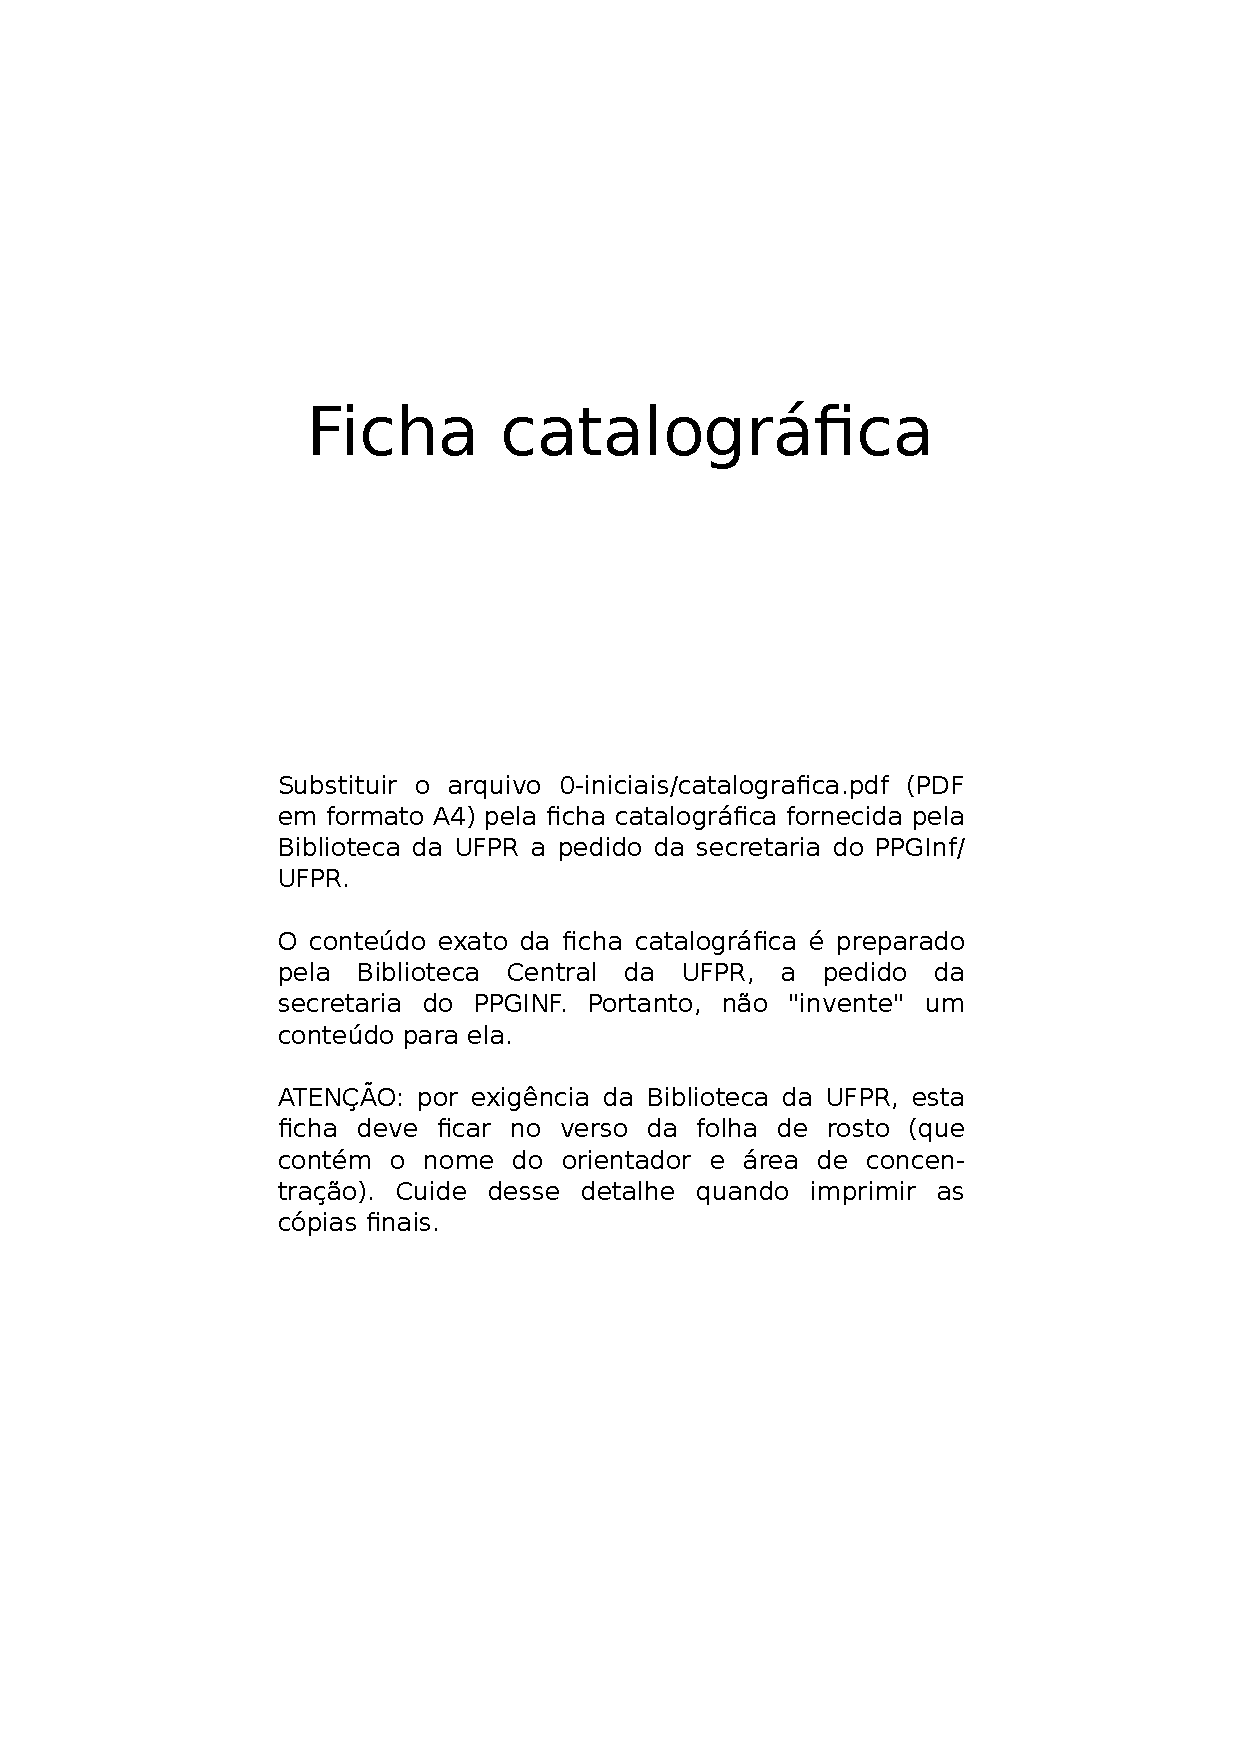
\includepdf[noautoscale]{0-preambulo/catalografica.pdf}

\end{ficha}

%=====================================================
		% ficha catalográfica
 % A ficha de aprovação será fornecida pela secretaria do programa,
% após a defesa e cumprimento dos demais trâmites legais.

\begin{aprovacao}	% só gera conteúdo se for na versão final

% inclusão do termo de aprovação final (arquivo PDF)
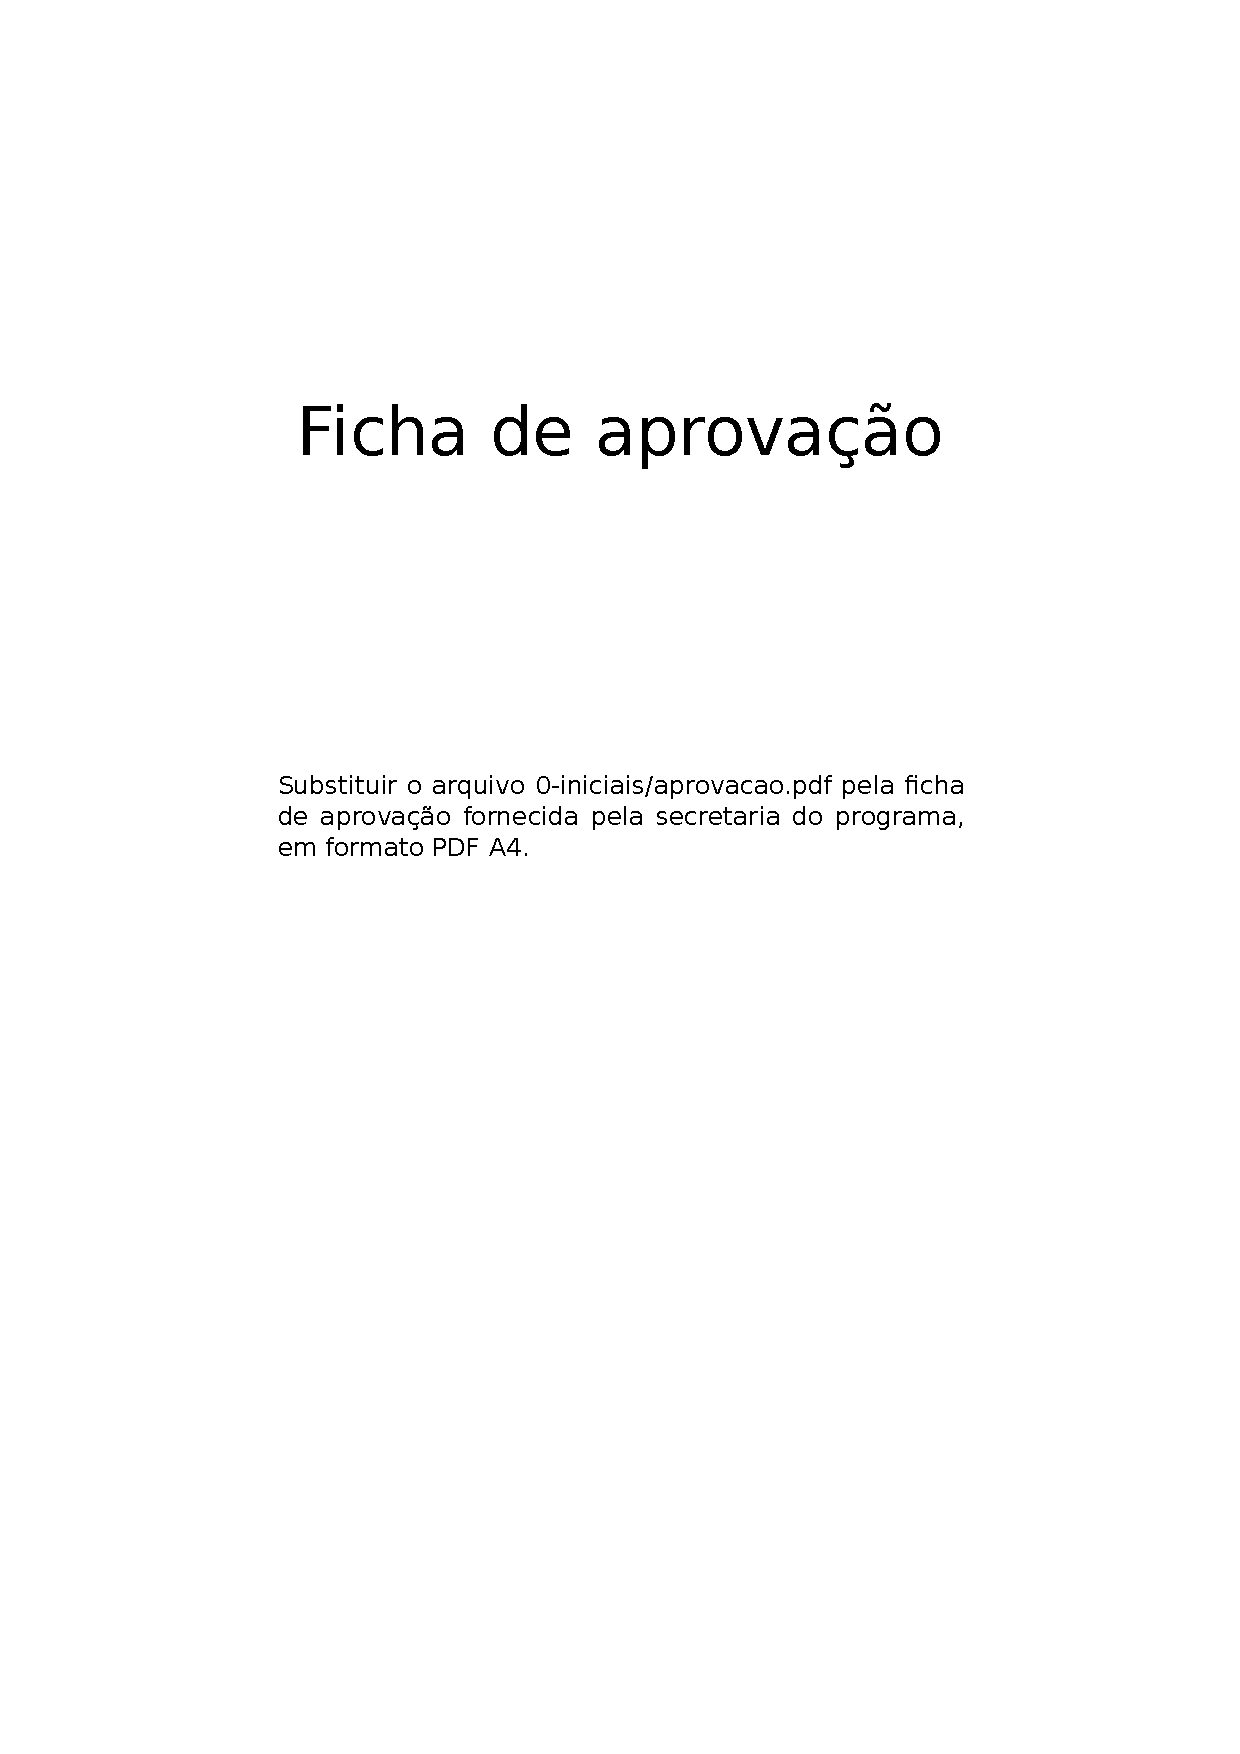
\includepdf[noautoscale]{0-preambulo/aprovacao.pdf}

\end{aprovacao}

%=====================================================
		% folha de aprovação
 \begin{dedica}  % só gera conteúdo se for na versão final

To my parents, who have stood by me all the way through.

\end{dedica}

		% dedicatória
 \begin{agradece}	% só gera conteúdo se for na versão final

%Several people have guided, aided and supported me throughout the research that led to this dissertation.

I would like to express my deep gratitude toward my advisor, Professor Luiz Albini, for all the guidance he offered throughout the research that led to this dissertation.
His frequent ideas and suggestions were what inspired me to pursue knowledge and be encouraged to find solutions to problems that are far from simple.

Furthermore, I would like to thank Professor Eduardo Todt, who has helped me in ways beyond this dissertation, and my fellow students, Eric, Nelson and Ivan, who always brought interesting conversations.

I would also like to thank my friends, in particular Taiane, Cainã, Douglas, Lucas and Giancarlo for bringing joy to my life for many years.

Perhaps most importantly, I would like to thank my parents, Edison and Lizmari, who supported me throughout the whole process and always reminded me that I was on a path worth pursuing, as well as my grandmother Glacial and everyone in my family.



%Inserir os agradecimentos. Os agradecimentos devem ocupar no máximo uma página, devem ser justificados na largura da página e com um afastamento de parágrafo na primeira linha de 1,27 cm. O espaçamento entre linhas deve ser de 1,5 linhas. Não deve haver espaçamento adicional entre parágrafos.

%\lipsum[2-5]	% gera um texto aleatório

\end{agradece}

		% agradecimentos

% inclui resumo e abstract
\begin{resumo}

%O resumo deve conter no máximo 500 palavras, devendo ser justificado na largura da página e escrito em um único parágrafo\footnote{E também não deve ter notas de rodapé; em outras palavras, não siga este exemplo... ;-)} com um afastamento de 1,27 cm na primeira linha. O espaçamento entre linhas deve ser de 1,5 linhas. O resumo deve ser informativo, ou seja, é a condensação do conteúdo e expõe finalidades, metodologia, resultados e conclusões.

%\lipsum[11-14]	% texto aleatório

À medida em que computadores tornam-se menores e mais poderosos, a possibilidade de integrá-los a objetos do cotidiano é cada vez mais interessante.
Ao integrar processadores e unidades de comunicação sem fio a veículos, é possível criar uma rede veicular ad-hoc (VANET), na qual carros compartilham dados entre si para cooperar e criar ruas mais seguras e eficientes.
Uma solução descentralizada ad-hoc, que não depende de infraestrutura pré-existente, conexão com a internet ou disponibilidade de servidores, é preferida para que a latência de entrega de mensagens seja a mais curta possível em situações críticas.
No entanto, assim como é o caso de muitas novas tecnologias, VANETs serão um alvo de ataques realizados por usuários maliciosos, que podem obter benefícios ao afetar condições de trânsito.
Para evitar tais ataques, uma importante característica para redes veiculares é gerenciamento de confiança, permitindo que nós filtrem mensagens recebidas de acordo com valores de confiança previamente estabelecidos e designados a outros nós.
Para gerar esses valores de confiança, nós usam informações adquiridas de interações passadas; nós que frequentemente compartilham dados falsos ou irrelevantes terão valores de confiança mais baixos do que os que aparentam ser confiáveis.
Este trabalho propõe um modelo de gerenciamento de confiança no contexto de trajetos diários, utilizando o \textit{Working Day Movement Model} como base para a mobilidade de nós.
Este modelo de movimentação permite a comparação entre VANETs e redes sociais tradicionais, pois é possível observar que pares de veículos podem se encontrar mais de uma vez em diversos cenários: por exemplo, eles podem pertencer a vizinhos ou colegas de trabalho, ou apenas tomar rotas similares diariamente.
Através de repetidos encontros, uma relação de confiança pode ser desenvolvida entre um par de nós.
O valor de confiança resultante pode também ser usado para auxiliar outros nós que podem não ter uma relação desenvolvida entre si.
O algoritmo proposto é baseado em um já existente, que foi desenvolvido para redes centralizadas e focado em modelos ad-hoc estáticos; o algoritmo anterior será adaptado para servir uma rede descentralizada e dinâmica, que é o caso de VANETs.
Usando valores de confiança existentes, um grafo direcionado é modelado, no qual arestas representam a relação de confiança entre os pares de nós.
Então, componentes do grafo são formados, de forma que nenhum par de nós em um componente tenha uma relação de confiança negativa.
Um algoritmo de coloração de grafo é usado no grafo de componentes resultantes e, usando os resultados de coloração, é possível inferir quais nós são considerados maliciosos pelo consenso da rede.
Espera-se que o algoritmo completo final seja rápido, para que ele possa ser executado frequentemente, e permita que nós mantenham um modelo da rede ao seu redor indicando quais nós vizinhos podem ou não ser confiados.

\end{resumo}


\begin{otherlanguage}{english}

\begin{abstract}

% em inglês, o primeiro parágrafo não deve ser indentado
\noindent
As computers become small and powerful, the possibility of integrating them into everyday objects is ever more appealing.
By integrating processors and wireless communication units into vehicles, it is possible to create a vehicular ad-hoc network (VANET), in which cars share data amongst themselves in order to cooperate and make roads safer and more efficient.
A decentralized ad-hoc solution, which doesn't rely on previously existing infrastructure, Internet connection or server availability, is preferred so the message delivery latency is as short as possible in the case of life-critical situations.
However, as is the case with most new technologies, VANETs might be a prime target for attacks performed by malicious users, who may benefit from affecting traffic conditions.
In order to avoid such attacks, one important feature for vehicular networks is trust management, which allows nodes to filter incoming messages according to previously established trust values assigned to other nodes.
To generate these trust values, nodes use information acquired from past interactions; nodes which frequently share false or irrelevant data will have lower trust values than the ones which appear to be reliable.
This work introduces TruMan, a trust management model for vehicular networks in the context of daily commutes, utilizing the Working Day Movement Model as a basis for node mobility.
This movement model allows the comparison of VANETs to traditional social networks, as it can be observed that pairs of vehicles are likely to meet more than once in several scenarios: for example, they can belong to neighbors or work colleagues, or simply take similar routes every day.
Through these repeated encounters, a trust relationship can be developed between a pair of nodes.
The resulting trust value can also be used to aid other nodes which might not have a developed relationship with each other.
TruMan is based on a previously existing algorithm, which was developed for centralized networks and focused on static ad-hoc models; its concepts were adapted to serve a decentralized and dynamic network, which is the case of VANETs.
Using trust values formed by node interactions, a trust graph is modeled; its edges represent trust relationships between pairs of nodes.
Then, strongly connected components are formed so that each node in each component trusts other nodes in the same component directly or indirectly.
A graph coloring algorithm is used on the resulting components graph and, using the coloring results, it is possible to infer which nodes are considered malicious by the consensus of the network.
TruMan is fast, so it incurs low pressure on on-board computers, and is able to satisfy most desired properties for vehicular trust management models.

%With the possibility of integrating smart features into vehicles, 

%The abstract should be the English translation of the ``resumo'', no more, no less.

\end{abstract}

\end{otherlanguage}



% define sumário e demais listas (figuras, tabelas, abreviações/siglas, símbolos)
\tableofcontents
\listoffigures
%\listoftables
 %=====================================================

% lista de acrônimos (siglas e abreviações)

\begin{listaacron}

\begin{longtable}{ll}
DTN & Delay-Tolerant Network\\
GPS & Global Positioning System\\
LTE & Long-term Evolution\\
MANET & Mobile Ad-hoc Network\\
WDM & Working Day Movement Model\\
OBU & On-Board Unit\\
RSU & Road-Side Unit\\
V2I & Vehicle-to-Infrastructure\\
V2V & Vehicle-to-Vehicle\\
VANET & Vehicular Ad-hoc Network\\
WAVE & Wireless Access in Vehicular Environments\\






%DINF & Departamento de Informática\\
%PPGINF & Programa de Pós-Graduação em Informática\\
%UFPR & Universidade Federal do Paraná\\
\end{longtable}

\end{listaacron}

%=====================================================		% ainda deve ser preenchida à mão
 %=====================================================

% lista de símbolos

\begin{listasimb}

\begin{longtable}{p{0.2\linewidth}p{0.7\linewidth}}
$\delta$ & Network density (see \autoref{section:density}).\\
$\rho$ & Transmission range.\\
$\eta$ & Number of nodes in a network.\\
$\alpha$ & Area of a simulation.\\
$\pi$ & The constant pi.\\
%$\alpha$ & alfa, primeira letra do alfabeto grego\\
%$\beta$ & beta, segunda letra do alfabeto grego\\
%$\gamma$ & gama, terceira letra do alfabeto grego\\
%$\omega$ & ômega, última letra do alfabeto grego\\
%$\pi$ & pi \\
%$\tau$ & Tempo de resposta do sistema\\
%$\theta$ & Ângulo de incidência do raio luminoso\\
\end{longtable}

\end{listasimb}

%=====================================================
		% idem
 

%=====================================================

% define estilo do corpo do documento (capítulos e apêndices)
\mainmatter
\pagestyle{mainmatter}

\begin{resumoextendido}
		
	\section*{Introdução}
%	Computadores estão cada vez menores e mais poderosos, permitindo que diversos aspectos da vida possam ser melhorados ao adicionar unidades de processamento a dispositivos comuns.
%	Muitas dessas aplicações são focadas em conveniências, a integração de objetos com computadores pode ser usado para economizar tempo e salvar vidas \citep{rti2014}.
%	Uma forma de fazer isto é adicionando computadores e dispositivos de comunicação a veículos -- como carros, ônibus e trens -- para aumentar a eficiência e a segurança do trânsito.
%	
%	Em 2013, cerca de 1,25 milhão de pessoas perderam suas vidas devido a acidentes de trânsito \citep{whofactsheet}.
%	Nos EUA, este número tem diminuído ao longo das últimas décadas, mas ainda é uma grande causa de morte ao redor do mundo \citep{whotraffic}.
%	Além disso, com o aumento da população de veículos, congestionamento tomam muito tempo das pessoas em suas rotinas.
%	Em cidades como Los Angeles, Moscou, Nova Iorque, Bogotá e São Paulo, pessoas passam dezenas de horas por ano no trânsito \citep{inrixtraffic}.
%	
%	Veículos inteligentes e redes veiculares são ferramentas tecnológicas para remediar os problemas acima.
%	Através do uso de sensores e de comunicação sem fio, os veículos podem evitar acidentes ao alertar motoristas distraídos \citep{lee2004collision} ou ao acompanhar a velocidade e posição de outros veículos \citep{hafner2011automated}.
%	Além disso, podem sugerir rotas para distribuir o tráfego e evitar congestionamentos.
%	
%	Se tratando de aplicações de segurança e eficiência no trânsito, é crucial que comunicações ocorram com baixa latência (cerca de 100 milissegundos \citep{camp2005vehicle}).
%	Tecnologia celular contemporânea, como LTE, poderia ser usada para conectar veículos à internet, mas a latência adicionada pela transmissão tornaria aplicações de segurança lentas e pouco confiáveis \citep{mangel2010comparison}.
%	Outros potenciais problemas da tecnologia celular para o uso veicular incluem a necessidade de infraestrutura, o custo do serviço, e o compartilhamento da rede com outros tipos de dispositivos.
%	
%	Portanto, uma solução \textit{ad-hoc} é preferível, sem depender de infraestrutura e permitindo a comunicação direta entre participantes da rede.
%	
%	
%	Porém, como é o caso em muitas tecnologias novas, VANETs podem ser um alvo de ataques de usuários maliciosos.
%	Um usuário malicioso local pode alterar dados para manipular o trânsito, enquanto atacantes remotos podem invadir veículos para controlar a rede \citep{garip2015congestion}.
%	Ataques podem ser apenas inconveniências até ameaças à vida, portanto é importante que redes veiculares estejam preparadas para mitigá-los.
%	
%	Em redes \textit{ad-hoc}, uma forma de mitigar certos ataques é usando dados coletados previamente para filtrar mensagens que aparentam ser maliciosas, incorretas ou irrelevantes.
%	Para tal, emprega-se o conceito de \textit{confiança}.
%	Ao receber mensagens de outros nós, um membro da rede pode construir uma relação de confiança com os outros.
%	Caso o valor de confiança da origem de uma mensagem seja muito baixo, essa mensagem pode ser considerada não confiável.
%	Além disso, essas relações de confiança podem ser propagadas pela rede, permitindo que nós que ainda não formaram suas próprias opiniões possam se beneficiar da informação que já circula pela rede.
%	
	
	Dentro dos próximos anos, uma grande parte de novos veículos virão equipados com funcionalidades de comunicação.
	Essas funcionalidades permitirão o compartilhamento de dados com outros dispositivos e podem ser ferramentas importantes para reduzir o trânsito e o risco de acidentes.
	Acidentes de trânsito são uma das maiores causas de morte no mundo \citep{whofactsheet}, tornando necessárias soluções para melhorar a segurança nas ruas.
	
	O compartilhamento rápido de dados entre veículos permite, por exemplo, que veículos inteligentes alertem seus motoristas sobre condições de trânsito \citep{lee2004collision} e que veículos autônomos formem pelotões \citep{amoozadeh2015platoon}.
	
	Assim, surge a necessidade de redes veiculares \textit{ad-hoc} (\textit{vehicular ad-hoc networks}, ou VANETs), nas quais veículos são os nós ou membros da rede e compartilham informações entre si, sem depender da internet ou de infraestrutura.	
	Porém, como é o caso em muitas tecnologias novas, VANETs podem ser um alvo de ataques de usuários maliciosos.
	Um usuário malicioso local pode alterar dados para manipular o trânsito, enquanto atacantes remotos podem invadir veículos para controlar a rede \citep{garip2015congestion}.
	Ataques podem ser apenas inconveniências até ameaças à vida, portanto é importante que redes veiculares estejam preparadas para mitigá-los.

	Em redes \textit{ad-hoc}, uma forma de mitigar certos ataques é usando dados coletados previamente para filtrar mensagens que aparentam ser maliciosas, incorretas ou irrelevantes.
	Para tal, emprega-se o conceito de \textit{confiança}.
	Ao receber mensagens de outros nós, um membro da rede pode construir uma relação de confiança com os outros.	
	Caso o valor de confiança da origem de uma mensagem seja muito baixo, essa mensagem pode ser considerada não confiável.
	Além disso, essas relações de confiança podem ser propagadas pela rede, permitindo que nós que ainda não formaram suas próprias opiniões possam se beneficiar da informação que já circula pela rede.

	Este trabalho propõe um novo modelo de confiança, TruMan, para gerenciar relações de confiança em uma rede veicular.
	Usando o modelo proposto, nós de uma rede veicular podem rapidamente identificar quais outros nós são dignos de confiança ou não.
	Como redes veiculares são altamente dinâmicas, nós adquirem mais informações à medida do tempo e podem se beneficiar de propriedades sociais de VANETs para construir relações fortes com outros nós encontrados frequentemente.
	
	O modelo TruMan é baseado em outro já existente, chamado MaNI \citep{vernize2015malicious}, que era restrito para redes estáticas.
	Utilizando algoritmos de grafos, TruMan demonstra-se uma solução eficiente para o problema de gerenciamento de confiança em redes veiculares.
	
	As próximas seções são as seguintes.
	A \textbf{Revisão Bibliográfica} aborda os conceitos de redes complexas, redes sociais, redes tecnológicas e redes veiculares, além de estudos relevantes na área de confiança para redes veiculares.
	Em \textbf{Projeto e Implementação do TruMan}, os objetivos e hipóteses do TruMan são apresentados, além das explicações dos algoritmos que compõe o modelo.
	A seguir, \textbf{Avaliação do TruMan} mostra as ferramentas usadas para validar o TruMan e os resultados dos experimentos realizados.
	Por fim, a \textbf{Conclusão} contém os pensamentos finais sobre o projeto.
		
	\section*{Revisão Bibliográfica}
	
	Uma revisão do estudo de redes como um todo foi feito para o desenvolvimento de um novo modelo de confiança para redes veiculares.
	Esta seção introduz conceitos relacionados a redes complexas, redes sociais, redes tecnológicas e redes veiculares, incluindo o significado e importância de confiança em cada tipo de rede.
	Por fim, trabalhos relevantes relacionados à área de confiança em redes veiculares são apresentados.
	
	\subsection*{Redes Complexas}
	Redes complexas podem descrever diversos sistemas observados na natureza e na sociedade com \textit{vértices} (ou \textit{nós}) e \textit{arestas} \citep{newmannetworks}.
	Geralmente são dividas em quatro categorias:
	\begin{enumerate}
		\item \textbf{Redes Tecnológicas} são construídas para prover serviços. Exemplos incluem a Internet, a rede telefônica e redes de transporte.
		\item \textbf{Redes Sociais} são compostas de pessoas ou grupos de pessoas e a relação entre elas. Podem ser relações de parentesco, amizades, relações profissionais, etc.
		\item \textbf{Redes de Informação} são redes nas quais os nós são informações e as arestas são relações entre conjuntos de informações. Por exemplo, a World Wide Web é uma rede de informação que existe na Internet (que, por sua vez, é uma rede tecnológica).
		\item \textbf{Redes Biológicas} são as redes encontradas na natureza. Podem ser compostas de animais, células, conjuntos de seres vivos, etc.
	\end{enumerate}
	
	Confiança pode ser uma ferramenta útil em diversos tipos de rede para proteger seus participantes.
	Sob a perspectiva da ciência da computação, confiança pode ser definida como uma medida de quanta certeza um membro da rede tem de que outro membro se comporta de forma adequada e fornece informações válidas e/ou significativas \citep{sherchan2013survey}.
	
	\subsection*{Confiança em Redes Sociais}
	Redes sociais são aquelas formadas por pessoas e as relações entre elas. 
	Em uma rede social, é simples observar a importância de confiança, pois é algo usado por pessoas todos os dias para tomar decisões.
	De forma geral, essas relações de confiança também funcionam quando adaptadas ao meio digital, pois relacionamentos construídos no mundo real permanecem válidos.
	
	Uma característica importante de redes sociais é a possibilidade de transmitir confiança de um relacionamento para outro, formando o conceito de ``amigos de amigos'' \citep{boissevain1974friends}.
	Isso permite que pares de integrantes de uma rede social mantenham um laço de confiança mesmo que não se conheçam diretamente, graças a um elo de confiança em comum, permitindo rápida disseminação de informação.
	
	Em geral, redes sociais são estáticas.
	Mesmo que laços de confiança sejam criados ou terminados, o formato geral da rede tende a mudar pouco, graças a uma série de outros laços formados entre nós próximos ao evento.
	
	\subsection*{Confiança em Redes Tecnológicas}
	Em muitas redes tecnológicas, como na Internet, confiança é aplicada de maneira centralizada através de serviços que fornecem segurança a seus usuários.
	Ou seja, no contexto da Internet, confiança geralmente é derivada de uma fonte secundária; usuários e provedores de serviço raramente mantêm suas próprias listas de confiabilidade.
	
	Essas soluções são válidas para a Internet, mas seriam lentas demais para serem usadas em redes dinâmicas \textit{ad-hoc}.
	Redes \textit{ad-hoc} exigem soluções decentralizadas para gerenciamento de confiança.
	Ou seja, cada membro da rede armazena suas próprias opiniões sobre membros, originadas a partir de contatos anteriores.
	
	Além disso, como essas informações são adquiridas aos poucos, o conhecimento que um membro da rede tem é geralmente incerto e incompleto \citep{baras2005cooperation}.
	Raramente pode-se ter certeza de que determinada informação é completamente precisa.
	Por isso é importante também levar em consideração as informações adquiridas por vizinhos confiáveis, assim expandido o conhecimento disponível.
	
	Redes veiculares \textit{ad-hoc} são um caso especial de rede tecnológica, mas, devido a diversas peculiaridades em topologia e mobilidade, também apresentam peculiaridades quando se trata de confiança.
	
	\subsection*{Confiança em Redes Veiculares}
	Hoje, muitos veículos já vêm equipados com o hardware necessário para processamento e comunicação veicular.
	É esperado que, até 2022, a maioria dos veículos comuns também venham com tais funcionalidades \citep{connectedcar2016}.
	Redes veiculares \textit{ad-hoc} (VANETs) são uma aplicação muito estudada quando se trata de veículos inteligentes ou autônomos.
	Nelas, todos os nós são relacionados ao trânsito, como veículos ou unidades posicionadas em infraestrutura ao lado das ruas.
	
	O padrão de comunicação mais usado para redes veiculares é o IEEE 802.11p, que descreve dois tipos de membros (ou nós) para redes veiculares: unidades a bordo (\textit{on-board units} ou OBUs) e unidades de beira de estrada \textit(\textit{roadside units} ou RSUs).
	Comunicação entre pares de OBUs é denominada \textit{vehicle-to-vehicle} (V2V), enquanto comunicação entre OBUs e RSUs é chamada de \textit{vehicle-to-infrastructure} (V2I).
	Este estudo aborda apenas casos V2V e, portanto, refere-se apenas a veículos como membros de uma rede veicular.

	Como é esperado para novas tecnologias, redes veiculares podem se tornar um alvo relevante para usuários maliciosos e atacantes.
	Alguns exemplos de potenciais problemas são: 
	módulos e sensores, como GPS e velocímetro, defeituosos, inibindo aplicações de segurança ou eficiência \citep{isaac2010security}; 
	veículos intencionalmente transmitindo dados falsos \citep{golle2004detecting}; 
	atacantes remotos controlando múltiplos veículos para congestionar a rede \citep{garip2015congestion}; 
	invasão de privacidade ao tentar decifrar e ler mensagens alheias \citep{isaac2010security};
	disrupção de sinal para impedir a comunicação de outros veículos \citep{isaac2010security}.
	
	Como em outros tipos de rede, VANETs dependem de membros que se comportam de maneira correta e previsível e informações incorretas comprometem a utilidade da rede.
	Há uma distinção importante a ser feita entre nós maliciosos e defeituosos, porém, em termos de confiabilidade, é possível tratá-los da mesma forma, pois, afinal, a principal característica de ambos é a transmissão de informação incorreta.
	
	Em geral, soluções de gerenciamento de confiança são divididos em dois tipos: os que usam \textit{confiança orientada a entidade}, nos quais confiança é relacionada a membros da rede e leva-se em consideração quem transmitiu certa mensagem, ou \textit{confiança orientada a dados}, nos quais o conteúdo da mensagem é mais importante do que quem a transmitiu.
	Existem também algumas soluções que combinam ambos métodos.
	
	Algumas das propriedades únicas de redes veiculares, que afetam soluções de confiança para elas, são:
	topologia que muda constantemente e rapidamente;
	mobilidade de nós restringidas às ruas disponíveis;
	fragmentação, quando duas ou mais partes da rede estão distantes demais para se comunicar;
	comunicação pouco confiável com nós distantes;
	nenhuma restrição notável de energia, quando comparadas a redes de dispositivos móveis;
	densidade potencialmente muito alta;
	topologia suscetível a comportamentos erráticos de motoristas.
	
	Em \citep{zhang2011survey}, oito propriedades desejáveis para modelos de confiança para redes veiculares são apresentadas:
	construção de confiança descentralizada;
	lidar bem com baixas densidades;
	dinâmicas relacionadas a local, tempo, eventos e tarefas;
	escalabilidade;
	medida de certeza integrada;
	segurança a nível de sistema;
	sensibilidade a privacidade;
	robustez.
	
	\subsection*{Trabalhos Relacionados}
	
	Muitas soluções para confiança em redes veiculares foram propostas ao longo dos anos, como \citep{patwardhan2006data}, \citep{gerlach2007trust}, \citep{raya2008data}, \citep{huang2010situation}, \citep{ding2013novel}, \citep{haddadou2013trust}, \citep{liu2016lsot}, \citep{kerrache2016detection}.
	Além disso, alguns trabalhos oferecem revisões sobre propostas já apresentadas, como \citep{zhang2011survey}, \citep{ma2011survey}, \citep{zhang2012trust}, \cite{mejri2014survey}, \citep{soleymani2015trust}, \citep{sengar2016survey}, \citep{dwivedi2016review}.
	Nesta seção, alguns dos trabalhos mais relevantes são apresentados.
	
	No modelo proposto em \citep{minhas2010towards} usa diversos critérios para julgar se uma mensagem é confiável ou não.
	Ele utiliza uma combinação de confiança baseada em função (por exemplo, viaturas policiais são automaticamente mais confiáveis) e confiança baseada em experiência (baseada em interações anteriores).
	Além disso, uma mensagem é considerada mais confiáveis quando sua origem estava próximo do evento sendo relatado por ela.
	Quando múltiplas mensagens sobre o mesmo evento são recebidas, um nó pode optar por considerar as que foram enviadas por nós mais confiáveis, ou ponderar um consenso baseado em diversas opiniões alheias.
	Porém, este modelo depende apenas de interações diretas, e confiança não é propagada pela rede.
	
	Em \citep{chen2010trust}, os autores propõem avaliar mensagens com um método que utiliza grupos.
	Nós são separados em grupos e, cada vez que um deseja enviar uma mensagem, os outros membros do grupo oferecem suas opiniões sobre o emissor.
	Finalmente, um dos nós, designado como líder do grupo, coleta as opiniões e decide se a mensagem é válida de acordo com o consenso.
	Porém, é incerto como o modelo funcionaria em redes esparsas, manter grupos em uma rede altamente dinâmica pode ser uma tarefa de alto custo e um grupo todo pode ser comprometido se o líder não for confiável.
		
	O modelo ART \citep{li2016art} busca um modelo robusto e resistente a ataques.
	Ele tem dois passos principais: coleta de dados e detecção de nós maliciosos.
	Utiliza a teoria de evidências Dempster-Shafter para agregar dados vindos de outros nós.
	Então, usa uma métrica baseada em cosseno para comparar vetores de confiança de dois nós (cada vetor é uma sequência de opiniões que um nó tem sobre outros).
	Nós com vetores de confiança próximos confiam uns nos outros.
	O problema dessa solução é a dependência em cálculos custosos que podem atrapalhar o desempenho em situações que exigem baixa latência.
	
	Os autores de \citep{chen2017cloud} propõem uma solução de confiança baseada em nuvem, que exige um gerenciamento de confiança via internet.
	A vantagem disso é simplificar diversas dificuldades de redes veiculares, como redes esparsas e altamente dinâmicas.
	Contudo, o modelo é problemático em regiões com pouco ou nenhum sinal de comunicação celular e o sistema todo é suscetível a instabilidades no serviço.
	
	Por fim, é importante notar que nenhum dos trabalhos acima oferece análises de custo e complexidade de seus algoritmos.
	Portanto, manter uma baixa complexidade é um objetivo chave do modelo TruMan.
	
	\section*{Projeto e Implementação do TruMan}
	
	TruMan é um modelo de gerenciamento de confiança para redes veiculares, possibilitando a detecção de nós maliciosos em uma rede e a disseminação dados de confiança para outros nós.
	TruMan busca gerenciamento de confiança eficiente em redes altamente dinâmicas, mantendo baixo custo computacional e um modelo simples de entender e implementar.
	Esta seção apresenta os fundamentos e algoritmos por trás de TruMan, assim como detalhes de sua implementação.

	\textbf{Redes Sociais e VANETs}
	
	\subsection*{Algoritmo de Tarjan}
	
	O algoritmo de Tarjan para componentes fortemente conexos \citep{tarjan1972depth} é uma parte importante da eficiência atingida pelo TruMan.
	Este algoritmo permite abstrair um grafo grande em outro menor, reduzindo o custo de passos subsequentes.
	Dado um grafo direcionado $T = (V,E)$, um componente fortemente conexo é um grupo de nós nos quais, para cada par $u, v \in V$, há um caminho de $u$ para $v$ e de $v$ para $u$.
	Pensando em gerenciamento de confiança, podemos extender essa definição para considerar apenas caminhos formados por arestas que representam relações de confiança (ou um valor de confiança alto).

	O número de componentes é, no máximo, $|V|$: no pior caso, cada nó forma seu próprio componente.
	A complexidade do algoritmo é de $O(|V|+|E|)$.
	
	Utilizando os resultados do algoritmo de Tarjan, um grafo não direcionado $C = (V', E')$ é formado.
	Cada $v' \in V'$ representa um componente de $T$, enquanto as arestas $e' \in E'$ representam arestas entre nós de $T$ que não pertencem ao mesmo componente.
	
	\subsection*{Algoritmo de coloração de grafos}
	Coloração de grafos é um problema clássico da teoria dos grafos, no qual deve-se atribuir a cada nó uma cor de forma que não existam dois nós vizinhos com a mesma cor.
	Coloração de grafos é a heurística usada para a detecção de nós maliciosos no TruMan.
	Descobrir o menor número de cores possível para colorir um grafo arbitrário é um problema NP-difícil \citep{sanchez1989determining}.
	
	Os autores de \citep{mittal2011graph} apresentam uma solução eficiente de colorir grafos, apesar de não provar que o algoritmo sempre usa o menor número possível de cores.
	Porém, o algoritmo é eficiente e seus resultados são corretos, tornando-se extremamente útil para o TruMan.
	O custo do algoritmo é de apenas $O(|E|)$ -- em comparação, o algoritmo DSATUR tem complexidade de $O(|V|^2)$.
	
	\subsection*{O algoritmo TruMan}
	
	TruMan é baseado no algoritmo MaNI \citep{vernize2013dissertation}, que sugeriu o uso de componentes fortemente conexos e de coloração de grafos para a detecção de nós maliciosos em uma rede.
	Porém, o MaNI foi desenvolvido para redes estáticas e é executado por um agente externo à rede, tornando-se inapropriado para redes veiculares.
	Para funcionar em redes dinâmicas, TruMan roda iterativamente em intervalos pré-determinados.
	Além disso, o algoritmo roda de forma descentralizada, com uma instância rodando em cada membro da rede.
	
	Cada nó $u$ armazena um grafo direcionado de confiança $T = (V,E)$ que é uma abstração da rede real e começa apenas com $V = {u}$.
	Cada nó em $V$ representa um membro da rede e cada aresta em $E$ representa uma relação de confiança entre dois nós.
	Como cada nó armazena sua própria representação da rede e essa representação evolui com o tempo, há um $T_i^u = (V_i^u, E_i^u)$ para cada nó $u$ e iteração $i$.
	
	No começo de cada iteração, nós coletam informações sobre seus vizinhos.
	Um pré-requisito deste passo é a existência de um teste que classifica um nó adjacente como benigno ou malicioso.
	Tal teste é um problema grande por si próprio, e sai do escopo deste trabalho.
	Estudos sobre isso podem ser encontrados em \citep{golle2004detecting}, \citep{li2016defective}, \citep{kerrache2016detection}.
	
	Cada vez que um nó vizinho $v$ é identificado como benigno, o valor de confiança armazenado em $u \rightarrow v$ aumenta, e o grafo $T_i-1^v$ é unido com o grafo armazenado por $u$.
	Após coletar informações de todos os seus vizinhos naquele instante, um novo grafo $T_i^u$ é formado, que é utilizado para os próximos passos.
	
	Em seguida, $T_i^u$ é separado em componentes fortemente conexos usando o algoritmo de Tarjan \citep{tarjan1972depth}, de forma que cada par de nós em um componente é conectado por um caminho de confiança.
	Ou seja, todos os nós de um mesmo componente confiam uns nos outros direta ou indiretamente.
	Portanto, em termos de confiança, nós dentro de um mesmo componente podem ser considerados como um só: se um deles é confiável, pode-se assumir que todos são.
	Os componentes tornam-se nós do grafo $C^u_i = (V'^u_i, E'^u_i)$.
	
	O algoritmo de coloração de grafos \citep{mittal2011graph} é usado como heurística para classificar nós como benignos ou não.
	Após a execução do algoritmo, a cor cujos nós em $C_i^u$ representam a maior quantidade de nós em $T_i^u$ é classificada como correta, e as outras cores são classificadas como incorretas.
	Isto funciona porque, em uma rede na qual a maior parte dos nós são benignos, estes tendem a formar poucos componentes grandes, enquanto os nós maliciosos pertencem a componentes pequenos.
	Assume-se que a maior parte dos nós seja sempre benigna -- caso contrário, a rede como um todo está comprometida e perde completamente sua função.
	
	A complexidade do algoritmo pode ser calculada ao somar as operações mais custosas.
	Para cada iteração $i$ e nó $u$, e sendo $n$ o número de vizinhos de $u$, o cálculo é o seguinte:
	
	$$ TruMan = Tarjan + Colora\text{\textit{\c{c}}}\tilde ao + (Uni\tilde ao\times(n^u_i)) $$
	
	Como discutido acima, o algoritmo de Tarjan tem complexidade de $O(|V|+|E|)$ para o grafo de confiança $T$.
	Já o algoritmo de coloração tem complexidade de $O(|E'|)$ para o grafo de componentes $C$.
	A parte mais custosa do algoritmo é a união de grafos que acontece após a comunicação entre nós confiáveis.
	A complexidade desse processo é de $O(|E|)$ para vizinho que um nó tem em uma determinada iteração; o número de vizinhos é, no máximo, $|V|$.
	A complexidade total do Truman é, portanto:
	
	$$ O(|V|+|E|) + O(|E'|) + O(|V|\times |E|)$$
	
	Porém, $|E'| \leq |E|$ é sempre verdade, porque o grafo $C$ é uma redução do grafo $T$.
	Além disso, $|V|+|E| \leq |V|\times |E|$ também é verdade, com a exceção do cenário irrelevante no qual $|V| \leq 1$ ou $|E| \leq 1$.
	Portanto, a complexidade do algoritmo TruMan pode ser simplificada como:
	
	$$O(|V| \times |E|)$$
	
	\section*{Avaliação do TruMan}
	
	Para testar o TruMan, uma implementação do algoritmo foi feita usando Python.
	Grafos com mobilidade de nós foram gerados no simulador ONE \citep{keranen2009one}, usando o \textit{Working Day Movement Model} \citep{ekman2008working} para providenciar mobilidade próxima ao do mundo real, e um mapa de parte da cidade de Helsinki, Finlândia.
	Imagens da topologia da rede foram salvas a cada 10 segundos simulados, e essas imagens foram usadas como entrada para o algoritmo TruMan.
	O comportamento de nós maliciosos é aleatorizar suas opiniões sobre seus vizinhos.
	
	A maioria dos parâmetros da simulação no ONE foram tiradas do artigo do Working Day Movement Model \citep{ekman2008working}.
	Alguns parâmetros diferentes foram usados, mostrados na Tabela \ref{table:parameters}.
	Todos os nós da simulação são carros; para o propósito deste trabalho, nenhum outro tipo de veículo foi considerado.
	Uma parte pequena dos nós movimenta-se aleatoriamente, para simular veículos que não seguem padrões de movimento diários.
	
	O raio de transmissão dos nós varia de 10m a 50m, ilustrando as diferenças entre diferentes densidades de rede.
	A densidade de rede ($\delta$) é um valor que abstrai o volume e a frequência de conexões em redes veiculares, estimando a cobertura da rede pelo ambiente.
	Para o TruMan, densidades mais altas trazem melhores resultados, pois nós podem adquirir informações mais rapidamente.
	A densidade é calculada usando o raio de transmissão ($\rho$), o número de nós ($\eta$) e a área da simulação ($\alpha$).
	
	A cobertura de um único nó é o círculo ao redor dele formado pelo raio de transmissão.
	Esse valor é dividido por dois para compensar círculos sobrepostos, e então multiplicado pelo número de nós na rede.
	Por fim, esse valor é dividido pela área total do ambiente.
	A fórmula de densidade da rede é a seguinte:
	
	$$ \delta = \frac{\frac{\rho^2\pi}{2} \times \eta}{\alpha} $$
	
	As densidades de algumas simulações realizadas são exibidas na Tabela \ref{table:simdensities}.
	Já a Tabela \ref{table:citydensities} mostra as densidades de rede hipotéticas de algumas cidades do mundo, usando dados geográficos reais e supondo um raio de transmissão de apenas 10m.
	É possível ver que, mesmo com um raio de transmissão pequeno, as cidades oferecem densidades de rede maiores do que as das simulações, assumindo que uma parcela substancial de seus automóveis seja equipada com dispositivos de conexão.
	
	\subsection*{Simulações}
	
	Para validar o desempenho e a corretude de TruMan, diversas simulações foram executadas.
	
	A Figura \ref{fig:random103050} mostra simulações com 10\% dos nós agindo maliciosamente, com raio de comunicação entre 10m e 50m.
	É possível ver como o aumento do raio de comunicação melhora bastante os resultados:
	com 10m, quase 8000 iterações são necessárias para atingir um bom resultado, enquanto com 50 são apenas cerca de 1000.
	
	As Figuras \ref{fig:randommalicious1} e \ref{fig:randommalicious2} mostram simulações com quantidades diferentes de nós maliciosos e raio de comunicação de apenas 10m.
	Com até 30\% de nós maliciosos, os resultados são bons.
	Com 40\%, uma parte pequena de nós maliciosos não são detectados.
	Já com 50\%, os resultados são erráticos, pois o controle da rede é dividido entre os nós benignos e maliciosos.
	
	A maioria das simulações foram feitas com o limiar de confiança $h=0.5$, que significa que, para um nó confiar em outro, o valor de confiança deve ser acima de $0.5$.
	A Figura {fig:randomthresholds} demonstra o impacto de mudar esse limiar.
	Pode-se ver que o impacto não é muito significativo, porém, com $h=0.7$, os resultados são um pouco melhores.
	
	A Figura \ref{fig:random7} mostra os resultados da execução do algoritmo durante 7 dias simulados.
	A maioria dos nós maliciosos é detectada ao fim do primeiro dia, e a rede é completamente descoberta pouco tempo depois.
	Com o tempo, o número de falsos positivos cai, até tornar-se um número insignificante.
	
	Por fim, as Figuras \ref{fig:extramaliciousaging1} e \ref{fig:extramaliciousaging2} mostram como TruMan reage a um potencial ataque.
	Nessas simulações, um nó passa a ser malicioso na metade do tempo.
	O parâmetro $m$ determina quantas iterações o algoritmo leva para descartar arestas antigas, e, portanto, afeta a agilidade do modelo ao detectar um nó convertido.
	Com $m$ muito baixo, informações são descartadas muito rapidamente e o número de falsos positivos aumenta drasticamente.
	
	\section*{Conclusão}
\end{resumoextendido}
%\part{Dissertation}
% inclusao de cada capítulo, alterar a gosto (do professor de Metodologia...)
\chapter{Introduction} 	
\label{chap:introduction}
%=====================================================

% A introdução geral do documento pode ser apresentada através das seguintes seções: Desafio, Motivação, Proposta, Contribuição e Organização do documento (especificando o que será tratado em cada um dos capítulos). O Capítulo 1 não contém subseções\footnote{Ver o Capítulo \ref{cap-exemplos} para comentários e exemplos de subseções.}.


%=====================================================

As computers grow in power and shrink in size, more aspects of everyday life can be enhanced by adding processing units to common devices.
While many of these applications focus on conveniences, such as home automation \citep{mccole2016} (the collection of connected and smart devices is dubbed the Internet of Things or IoT \citep{morgan2014}), the integration of computers with other objects and devices can also be important to save time and save lives \citep{rti2014}.
One way of achieving this is by adding computers and wireless transmitters to vehicles — such as cars, buses, and trains — so they can share data which may increase traffic efficiency or reduce the chance of accidents \citep{saini2015close}.

In 2013, an estimated 1.25 million people lost their lives due to traffic accidents globally \citep{whotraffic}.
While this number has greatly reduced over the past decades \citep{johnson2010traffic} thanks to better safety features (seat belts, air bags, ABS, etc.) and stronger laws (drunk driving, motorcycle helmets, speed limits, etc.), it may still rise as a major cause of death in the years to come \citep{whofactsheet}, so further actions are necessary.
Furthermore, as the car population increases, congestions consume ever more time of the daily commuter, peaking at over 100 hours per year for the residents of Los Angeles, CA \citep{inrixtraffic}.

Smart vehicles and vehicular networks are ways that technology can aid both of the aforementioned problems.
Through the use of sensors and wireless communications, these vehicles are able to avoid accidents by alerting distracted drivers \citep{lee2004collision}, or by knowing in advance another vehicle's position and speed \citep{hafner2011automated}.
By communicating, they can also collaborate to offer driving and route suggestions, therefore reducing the possibility of traffic jams \citep{knorr2012reducing}.
%These features are possible with the development of a vehicular ad-hoc network (VANET), in which vehicles can quickly share data amongst themselves without the need of a server or an Internet connection.

When dealing with safety or traffic-efficiency applications, it is crucial that network communications occur with low latency (approximately 100 milliseconds \citep{camp2005vehicle}).
Current cellular technology, such as LTE, could be used to connect vehicles to the Internet, but the delay added by the transmission would make safety applications unfeasible or unreliable \citep{mangel2010comparison}.
Cellular connections also have other problems: the connection would require an active subscription with a carrier; the connection depends on available infrastructure; the wireless frequency would be shared with phones and other mobile devices, increasing the possibility of interference and congestion; server-side issues could impact the vehicles' communications.

For these reasons, ad-hoc solutions are preferred over centralized ones.
An ad-hoc network is one that has no reliance on pre-existing infrastructure (such as routers or access points) \citep{wu2004ad}.
Instead, each node is able to communicate directly with others and a routing protocol allows for messages to be forwarded until they reach their destinations.
Every time a node wants to send a message and the recipient is not a direct neighbor, it must choose which nearby node is the most likely one to get the message to its destination.
Routing techniques can use either the network's topology or geographical coordinates \citep{saini2015close} to choose which node should be the next hop.

These issues — the additional safety and efficiency as well as the low-latency communications — can be tackled through the use of a vehicular ad-hoc network (VANET), in which vehicles share data amongst themselves without relying on external devices, an Internet connection or server availability.
Neighboring vehicles can share their position and velocity data at high frequencies, allowing, for example, for autonomous vehicles to plan a platooning approach to traffic \citep{amoozadeh2015platoon}.
In the case of a collision or other event, nearby nodes can broadcast alerts, which other nodes pick up and forward \citep{li2007routing}.
That way, an alert can travel long distances in little time, allowing approaching vehicles to safely slow down or pick alternative routes.

\begin{figure}[h]
    \centering
    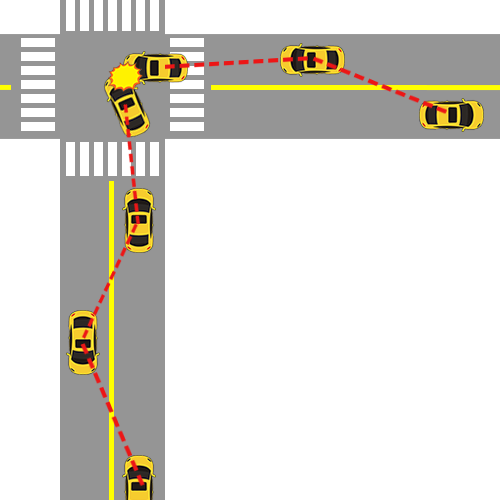
\includegraphics[width=0.5\textwidth]{images/collision.png}
    \caption{Propagation of a collision alert in a VANET}
    \label{fig:collision}
\end{figure}

As is the case with most new technologies, VANETs are expected to be a notable target of attacks for a diversity of reasons \citep{isaac2010security}.
A local malicious user might alter the data his or her vehicle broadcasts in order to manipulate traffic conditions, while remote attackers could invade vehicles' computers and obtain partial control of the network  \citep{garip2015congestion}.
These attacks can vary from time-consuming annoyances to life-threatening, so it is important that real-world implementations of vehicular networks are prepared to handle them.

%However, as is the case for many types of networks, VANETs must be reliable in order to be functional.

%In the case of ad-hoc networks, the nodes themselves must be reliable, since data can only propagate safely through benign cooperation.

%In ad-hoc networks, the secure propagation of data depends on the reliability of each node, since messages often travel 

%While in a conventional technological network (such as the Internet), the 
In ad-hoc networks, one way to mitigate a number of attacks is through each node using data collected from previous experiences to filter out incoming messages that seem to be malicious, incorrect, or irrelevant.
A node's degree of confidence that some data is correct and useful is called \textit{trust}.
%The ability of nodes to verify one another and judge messages based on past experiences is called \textit{trust}.
% The product of a series of past experiences with one other node is called trust.
For instance, in the example of a single malicious user broadcasting false data, nodes receiving these messages can use their own sensors to verify whether or not the data was correct, and update the \textit{trust value} of the sender vehicle.
In case the trust value of a sender is too low, a receiver node can choose to ignore the data contained in a message, as it concluded that the sender is not trustworthy.
Trust allows for better cooperation of nodes in a network, since incorrect messages might be detected and discarded.

Furthermore, once nodes form their own opinions about others, they can propagate pre-existing trust values when necessary.
For example, if two nodes are not direct neighbors and do not have any pre-existing trust information about each other, they can ask intermediary nodes for their opinions on the other node \citep{wang2009trust}.
The management of trust values (i.e. how one node acquires and updates trust values) and the use of these values to derive further information (such as designating nodes as malicious or not) is called \textit{trust management} \citep{ma2011survey}. 
%The combination of one node's trust of another with the opinions of other nearby nodes form what is called \textit{trust management}.
The effective use of trust management allows for the detection of malicious, misbehaving or faulty nodes in the network, and for such information to be shared amongst the benign participants. 
Throughout this document, trust and trust management may be used interchangeably.

%There is an important distinction between \textit{trust} and \textit{trust management}.
%The former relates to the actual trust relationship between a pair of nodes, while the latter concerns the management of previously generated trust data, such as previous tests or information received from neighboring nodes, and how this data can be used to make decisions.
%While this work addresses trust management rather than trust itself, both terms will be used when referring to trust management for the sake of brevity.
%Without trust management\footnote{} features, a vehicle cannot judge whether or not received messages are benign or malicious in order to make an informed decision and, therefore, incorrect data might be presented to the driver.

While the detection of incorrect nodes and/or messages is an important aspect of security and safety in vehicular networks, it does not address all of the problems.
Trust solutions are not viable without a solid identity verification scheme, for instance, since nodes would not be able to form trust opinions without being sure of the others' identities (these schemes often use a Public Key Infrastructure \citep{wasef2010complementing}).
They also do not address issues such as driver and passenger privacy when using the facilities of a VANET.
Furthermore, cryptography must be used in order to guarantee that the secrecy of messages is not violated.
Therefore, trust and trust management must be viewed as an important aspect of vehicular ad-hoc networks, but not as a definitive solutions to all of the related concerns.

In order to study the implications of trust in vehicular networks, it is interesting to first take a closer look at trust in other kinds of networks.
VANETs are a subset of technological networks, therefore it is useful to consider how the Internet or other ad-hoc networks handle trust.
Furthermore, VANETs contain several features often found in social networks, which can be directly tied to how nodes form and develop trust relationships with each other.

%While this work emphasizes on the characteristics of VANETs, they are only a subset of the much broader field of complex networks.
%The study of complex networks dates back decades, including analysis of biological or social networks \citep{wang2003complex} \citep{newmannetworks}.
%Trust issues are present in many of these types of networks, although each one requires a specific approach that addresses the peculiarities involved.

%Often, when people hear the term ``network'', they think only of technological examples, such as computer networks.
%Such networks are only a subset of a much larger field of study: that of complex networks.
%The study of complex networks dates back decades, including analysis of biological or social networks \citep{wang2003complex} \citep{newmannetworks}.
%Technological networks, and VANETs by extension, are only a subset of that much larger field of study.
%
%Trust issues and their solutions are an important aspect of the study of complex networks, and of social or technological networks in particular.
%Each different type of network requires a specific approach to trust, according to the features that distinguish it from others.
%It is interesting to review the solutions proposed for social networks and technological networks in general, and then narrow down on how dynamic networks, and VANETs in particular, are handled.
%Despite the differences, there are some concepts that overlap across most types of networks.

The study of networks is tied to graph theory, since graphs are a useful way to generate models of networks, and therefore many concepts of the two fields overlap.
Mathematical, computational and statistical concepts developed for graphs can be translated to be useful for a variety of different types of networks.
%, like, for example, finding articulation vertices in a graph to locate bandwidth bottlenecks in a computer network.
Therefore, this document utilizes notation from graph theory in order to represent various kinds of networks.

This work introduces TruMan, a trust management solution for vehicular networks. 
TruMan combines solutions to two classic graph theory problems, strongly connected components and graph coloring, in order to provide an efficient approach to identifying malicious nodes in a dynamic and decentralized network.
This is based on a previously existing algorithm, called MaNI \citep{vernize2015malicious}, which is limited to centralized networks.

In order to function in a dynamic and decentralized environment, TruMan takes advantage of features that allow the development of trust relationships between members of the network.
Since there is no unifying agent supervising the network, trust relationships are built over time, as nodes move around the network and meet other nodes.

These features are discovered by tracing analogies with social networks.
For example, certain groups of nodes might come into communication range of each other with predictable frequency, such as vehicles which belong to family members, neighbors or work colleagues as their owners perform their daily activities.
By considering such features, TruMan allows the formation of strong trust relationships,  which in turn facilitate the discovery of malicious members of the network.

%This work proposes a method for identifying malicious nodes in a vehicular network, although it may also be viable for other dynamic and decentralized networks.

%In order to adapt the algorithm to a dynamic and decentralized environment, it is necessary to locate network features that allow for trust relationships to be developed amongst the network members over time, since there is no centralizing agent to store and process the whole network's trust values.
%These features are found by tracing analogies to social networks, i.e. identifying how and why two nodes (in the case of VANETs, vehicles) would meet more than once and at a somewhat predictable interval.

% Seems like there's a paragraph missing to explain why we mention social and technological networks at all.

%Further explain VANETs

%VANETs can be complex networks

%why mention social networks

%\section{Document organization}
The remainder of this document is organized as follows. \Cref{chap:complexnetworks} explains the broad study of complex networks and the importance of trust in technological and social networks.
Then, \autoref{chap:vanets} goes into details regarding VANETs and the importance of trust solutions in the field, presenting previous studies made on the subject.
\Cref{chap:truman} describes the goals of TruMan, its underlying hypothesis and the work done to achieve those goals, as well as the previously existing algorithms which form parts of TruMan.
Next, \autoref{chap:simulations} explains the tools used to validate TruMan's functionality and presents the results of the experiments that were performed.
Finally \autoref{chap:conclusion} presents the final thoughts on the project and concludes this document.

%Finally, \autoref{chap:proposal} shows the fundamentals of this proposed work, including the similarities found between VANETs and social networks, a realistic movement model that may be used for simulations, the previously existing study on malicious node identification for complex networks, and the important aspects that must be adapted to the dynamic vehicular environment.			% introdução
\chapter{Complex Networks}
\label{chap:complexnetworks}

Complex networks can describe many systems which are observed in nature and society \cite{newmannetworks}, such as computer networks, food chains, protein structures, etc. 
They are generally divided into four categories:

\begin{enumerate}
	\item \textbf{Technological Networks} are grids purposefully engineered to provide services to consumers and/or citizens.
	 	The primary examples of these networks are the Internet, the telephone network, power grids, transportation and delivery networks.
	 	A commonly studied type of technological network are Mobile Ad-hoc Networks (MANETs), networks of mobile devices which communicate with each other without the need of a centralized agent.
		Although not of widespread use, MANETs can provide a way to create a network without pre-existing infrastructure, as long as each device is equipped with the proper hardware and software.
		In \autoref{chap:vanets}, a special type of MANET will be introduced, along with several details regarding trust in those types of networks.
	\item \textbf{Social Networks} are formed of relationships between people, or groups of people.
		These relationships can be familiar, friendships, acquaintance, etc.
		For the purposes of this work, the most relevant type of relationship is that of trust.
		The details surrounding trust relationships in social networks are shown in \autoref{section:trustsocial}.
	\item \textbf{Information Networks} are the ones in which nodes are pieces of data or information and the edges are the connections between those pieces.
		Often, information networks are directly associated with technological or social networks.
		For instance, while the World Wide Web is an information network (in which the nodes are webpages and the edges are the links that users click on to navigate), it relies on the Internet, as is contains the physical infrastructure that makes the web possible.
		Online social networks can also be classified as information networks, since their nodes are actually information about people rather than the people themselves.
	\item \textbf{Biological Networks} are the networks found in nature.
		Their nodes can be chemicals, cells, animals, groups of lifeforms, and more.
		The brain contains a neural network formed by neurons, cells which enable information processing; connections in the network represent signals that are sent from one neuron to another.
		Another instance of biological networks are food chains, categorized as ecological webs.
		Species of animals are the nodes, while the predation of other species form the edges.
		
\end{enumerate}

As this work relates to trust issues in complex networks, it is interesting to further examine social networks and the importance of trust within them.
While the end result of the study will be applied to technological networks, certain aspects of social networks provide useful analogies to trust management in other kinds of networks.

\section{Trust in Social Networks}
\label{section:trustsocial}
In a traditional social network, it is simple to perceive how trust is relevant and how it works, since trust relationships between people (friends, relatives, colleagues, etc.) are used on a daily basis to make decisions.
When adapted to a digital environment, these social relationships can be used to automatically increase the relevance of certain information.
For instance, upon reading an online review for a certain product, a user will be more likely to accept the review's conclusion if it was written by a close friend than if it were written by a stranger.
Furthermore, if the review was written by a person who the user knows to be malicious or uninformed, its contents will be even less relevant.
In short, trust is a way of estimating how much a certain recommendation will lead to a positive outcome. \cite{golbeck2006inferring}

Social networks also have the property of carrying trust from one relationship to another:
information shared by a close friend of a person might be considered almost as trustworthy as some collected by the person him or herself.
Therefore, it is possible to model social trust relationships as a graph, in which nodes represent people and edges represent a certain degree of trust.
Friends of friends \cite{boissevain1974friends} might not have very high trust values, but could still be considered more trustworthy than the average stranger.
This property is similar, but not identical, to transitivity, since trust is diminished for each extra step an origin node needs to reach a destination, and there is also the possibility that one node distrusts another even if they share a mutual friend.

Social networks also have the trait of being mostly static.
Although friendships are formed and ended frequently, those connections do not disrupt the general shape of the network.
In fact, the ending of a friendship might indicate the presence of a \textit{negative} trust relationship between two people.
Such negative information can be useful in digital social networks since, frequently, only positive relationships are available.
% \textemdash for example, on Facebook, people are usually only connected if there is a positive relationship between them.

Many works exist regarding trust relationships in complex networks, and in social networks in particular.
Here, only a few examples will be described, in order to show the general idea of trust research for these types of networks.



\section{Trust in Technological Networks}

%=====================================================
		% redes complexas
\chapter{Vehicular Ad-hoc Networks}
\label{chap:vanets}

Today, most premium vehicles come equipped with hardware that allow for connectivity features; it is expected that, by 2022, many standard vehicles will also come with such features built-in, accounting for a substantial share of the automotive industry's revenue \citep{connectedcar2016}.
Although these features can be useful tools to aid drivers, reducing traffic and risk of accidents, they are merely a gateway to the long-term goal of truly autonomous vehicles, which might become a reality within the next decade; many automakers and technology companies have laid out their plans for the upcoming years \citep{tesla2016}.
However, the proper functioning and utility of both connected and fully autonomous vehicles rely on technologies, protocols and applications that allow for the fast communication between vehicle's on-board computers.

Vehicular ad-hoc networks, which are a special instance of MANETs, are a much-studied solution to the problems in the way of smart and autonomous vehicles.
In these networks, all nodes are related to traffic; they can be vehicles equipped with on-board computers, or stationary units placed near roads.
By quickly sharing data with neighboring vehicles, without the need of an Internet connection, smart vehicles can alert their drivers of important road conditions \citep{barba2012smart}, while autonomous vehicles can synchronize their movements to maximize traffic throughput \citep{amoozadeh2015platoon}.

%The advantages of an ad-hoc approach, as opposed to using cellular infrastructure or other server-based solutions, are explained in \autoref{chap:introduction}.
%For messages to travel to nodes out of the sender's wireless range, they must use other nodes as \textit{hops}.
%This approach requires appropriate routing protocols that consider the dynamic topology of VANETs.
%While traditional MANETs often use protocols which rely on the network topology, the ones proposed for VANETs generally use geographic position instead \citep{saini2015close}; these protocols use GPS coordinates in order to send messages to the available neighbor physically closest to the destination node.

%Certain cars available for purchase today are able to achieve some of those features (including autonomy) through a variety of sensors (cameras, accelerometers, microphones, etc.) which capture information about the world around them.
%However, these sensors don't provide a complete solution, since they are subject to a variety of interferences.
%The combination of built-in sensors with connectivity may provide the 

%The prospect of autonomous vehicles makes the study of Vehicular Ad-hoc Networks (VANETs) important.
%However, it will still take many years before completely autonomous vehicles are the norm and, until then, VANETs can be a valuable tool to help drivers reduce travel times and diminish the risk of collisions.
%Thousands of people die each year due to traffic accidents, many of which could have been avoided if vehicles were smarter and able to provide important alerts both to their drivers and to neighboring vehicles.
%The vehicles' on-board computers can aid drivers to increase safety and reduce traffic, but data needs to be shared among the various vehicles in the network.
%Such data includes location, speed and destination, which neighboring vehicles can use to adjust their trajectory and increase their own efficiency.
% By allowing vehicles to share their locations, speeds, and destinations with each other, traffic can become more stable and predictable.

\begin{figure}[h]
    \centering
    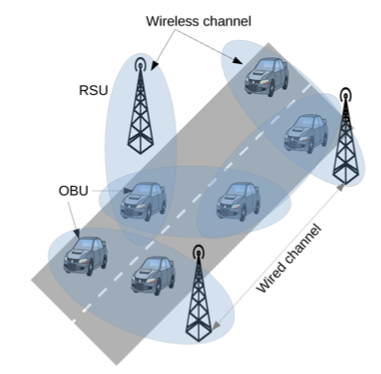
\includegraphics[width=0.5\textwidth]{images/vanet.png}
    \caption{Basic elements of a VANET: OBUs and RSUs. \citep{saini2015close}}
    \label{fig:vanet}
\end{figure}

Several current efforts to make VANETs viable in cities are centered around the IEEE 802.11p standard, also called Wireless Access in Vehicular Environments (WAVE) \citep{jiang2008ieee}.
Among other aspects of the wireless technology, the WAVE standard describes two types of nodes for vehicular networks: on-board units (OBUs) and road-side units (RSUs).
On-board units are computers placed within each vehicle which monitor the vehicle's data and are able to communicate with other nodes using wireless signals.
Road-side units are placed in static locations near roads; they may also have wired interfaces with other RSUs and the Internet, so it is possible to use them as anchor points for Internet access for passing vehicles.
When referring to the communication between two OBUs, the term vehicle-to-vehicle (V2V) communication is used \citep{yang2004vehicle}; when both an OBU and an RSU are involved, it is called vehicle-to-infrastructure (V2I) communication \citep{chou2009feasibility}.
Although this nomenclature is important to understand other studies on the subject of VANETs, this study does not consider RSUs and focuses only on vehicles themselves as nodes, so references to VANETs and vehicular networks are exclusively tied to V2V communications.

%When referring to VANETs, the terms vehicle-to-vehicle (V2V) and vehicle-to-infrastructure (V2I) are used.
%Both are types of communications that may occur within vehicular networks, depending on which nodes are actively participating in the networks.
%Aside from the vehicles themselves, VANETs can use road-side infrastructure to provide additional features, such as Internet access, to its users.
%In the model proposed in this work, however, such infrastructure is not used, so references to VANETs and vehicular networks are exclusively tied to V2V communications.

%[description of trust in context of VANETs]

In traditional networks (ad-hoc or not), routing protocols usually use the topology to choose where to forward packets; in other words, the primary metric used is the number of hops required to reach the destination.
This metric is not as useful in vehicular networks, since the high mobility causes the topology to change frequently.
Instead, most VANET routing protocols use geographical coordinates to forward packets \citep{saini2015close}, that is, the physical distance between two nodes is used as the primary metric.
The implication is that, even if a packet requires more hops to reach its destination, it will always be traveling the generally correct direction.

%[Explain basic security features]

As expected for a new technology being introduced, vehicular communications can become an appealing target for malicious users and attackers.
These are some examples of possible issues in a VANET:

\begin{enumerate}
	\item 	Vehicles with faulty GPS modules, speedometers or other sensors.
			If a vehicle is broadcasting incorrect data (perhaps unknowingly) because of a hardware or software fault, it can be a serious hinderance to efficiency and safety applications.
			It might behaving appropriately according to protocol, but the data it sends is not reliable \citep{isaac2010security}.
	\item	Vehicles might be deliberately broadcasting false data.
			In this case, there might be a specific purpose (by either the vehicle's driver or a remote attacker), like altering traffic or even cause an accident \citep{golle2004detecting}.
	\item   Attackers with control of several vehicles can propagate junk data in an attempt to flood the network, causing a distributed denial of service (DDoS) attack.
			Alternatively, the data propagated might have some reasoning behind it, like lying about road conditions in order to divert traffic \citep{garip2015congestion}.
	\item	Instead of sending data, some vehicles might try to eavesdrop on others' communications.
			The hop-based routing protocols used in VANETs facilitate this, since any node can be asked to be a hop.
			If the intermediary node is malicious, it may attempt to extract data contained in messages or refuse to forward them.
			Related to this, there is the Sybil attack \citep{isaac2010security}, in which a node lies about its position in order to seemingly alter the physical topology of the network and be chosen as a hop \citep{leinmuller2005influence}.
	\item	Malicious vehicles may use signal jammers or other devices in order to affect other vehicles' sensors and communications \citep{isaac2010security}.
			That can cause other vehicles to broadcast incorrect data, therefore obfuscating the origin of the attack.
	\item	A malicious user or remote attacker can monitor messages shared across the network in an attempt to stalk one specific vehicle \citep{isaac2010security}.
	
\end{enumerate}

Each of these possible attacks requires a unique approach, though there are some broader ways to help the security and safety of VANET users.
Trust, as is described in \autoref{section:trustvanet}, can be an important feature in vehicular networks, especially when attempting to filter out malicious or incorrect messages.
It does not, however, avoid all possible attacks, such as a signal jammer or stalking.
Rather, different mechanisms must be explored in order to avoid most problems.

%Related to trust is the issue of identity in vehicular networks.
%Solutions to this issue can be important elements of security and privacy, and there are studies focusing on node identification in VANETs (that is, making sure a node is who it claims to be), in particular through the use of a Public Key Infrastructure (PKI) \citep{wasef2010complementing}.
%In fact, at least one study proposes that these identities must be refreshed with a certain frequency to maintain the privacy of each node \citep{golle2004detecting}.
%However, refreshing identities can make maintaining a trust relationship between two nodes difficult or even impossible, since there is no way to know which nodes changed identities.
%Although it is important that nodes are not able to lie about identity and are able to maintain their privacy, persistent identities is a prerequisite for the model proposed here.

% While certification of identity is an issue in vehicular networks, and , this work will not address it.
%There are studies focusing on node identification in VANETs (that is, making sure a node is who it claims to be), in particular through the use of a Public Key Infrastructure (PKI) \citep{wasef2010complementing} 
%\citep{kumar2015intelligent}.
%One study proposes that such identities must be refreshed with a certain frequency to maintain the privacy of each node \citep{golle2004detecting}.
%Although it is important that nodes are not able to lie about identity and are able to maintain their privacy, nodes having valid identities that are persistent over time, so that nodes can identify each other over a long period, is a prerequisite for the model proposed here.


\section{Special properties of VANETs}
\label{section:properties}
%As was described above, VANETs are a special type of MANETs, which in turn are technological networks.
%However, 
VANETs feature several unique properties which distinguish them, and the behavior of its members, from other types of networks \citep{yousefi2006vehicular}.
Some of these properties include:

\begin{enumerate}

	\item 	Rapidly changing topology.
			Since the nodes are vehicles, they move frequently and at relatively high speeds.
			Each node's wireless communications also have a certain range, so the other nodes within that range (and, therefore, network neighbors) can change very quickly.
%			To build a topology model of its surrounding network, a node must often ping its neighbor to gather information.
%			Using velocity and location information, however, it is possible to create reasonable assumptions about future states of the topology.
			
	\item	Node mobility is constrained to a pre-existing grid of roads.
			Within those roads, nodes usually travel in predictable directions according to local laws and historical data.
			The spaces in the grid, like city blocks, provide a challenge to communication both because of distance and because buildings can cause obstructions to radio transmissions.
			
	\item	VANETs are prone to fragmentation, since a gap in the network topology can make two parts of it unable to communicate with each other.
			Combined with the property above, this fragmentation can appear and disappear frequently, depending on the node density.
			
	\item	Due to the changing topology and possible disconnection, connection with distant nodes is not reliable.
			Therefore, the effective diameter of the network is relatively small for important applications.
			
	\item 	Compared to devices like smartphones, vehicles have no notable power constraints.

	\item 	In certain locations and/or moments, large vehicle density results in a large-scale network, since there are many nodes concentrated in a relatively small space.
	
	\item 	The topology is susceptible to driver behavior.
			First, this means the topology can occasionally change in unpredictable ways.
			Second, contents of a message sent through the network can alter the driver's behavior and therefore change the topology.
			
\end{enumerate}

Some of these properties provide advantages or disadvantages when developing trust models for vehicular networks, although all of them must be considered.

\section{Trust in VANETs}
\label{section:trustvanet}
Like in other types of networks, the proper functioning of a VANET depends on the reliability of the vehicles (nodes) which participate in it.
If a node is malicious or faulty, it can spread incorrect data that may compromise the network's utility.
Once the concept of VANETs was established, researchers have been attempting to predict ways in which malicious users might use the network to their advantage.
Examples include triggering false alarms about inexistent accidents, lying about the average speed in a road to make it less desirable for others, and falsifying geolocation data to exploit location-based routing algorithms.
Therefore, the concept of trust must be established in the vehicular network context, allowing for nodes to judge the validity of information transmitted by others and share those conclusions with other nodes.

There is an important distinction between a malicious node and a faulty one; both of them may be sharing false data, but for different reasons and with different consequences.
For example, a malicious node may lie about its location in order to make routing protocols use it \citep{leinmuller2005influence}, in order to try to store or alter messages, while a faulty GPS module may cause an accident because its position data was incorrect.
However, that distinction can be hard to make, because a close inspection is necessary to determine whether the incorrect data is erratic or deliberate.
Since both types of nodes are problematic to the proper functioning of a network, malicious and faulty nodes can be treated as the same in a trust model.

%\textbf{/*********}
%Trust can be a related, yet distinct, issue to cryptography and authentication in vehicular networks.
%Many studies propose the use of a PKI (Public Key Infrastructure) to guarantee legitimate identities for nodes, although this solution requires, by definition, a certifying authority to manage and distribute public keys.
%VANETs must be able to function in a completely independent fashion, regardless of the amount of active nodes in a given region, and without relying on a centralized service.
%Both trust and authentication must work together to provide an adequate solution for VANETs, since it is difficult to establish trust without means to verify an identity (a malicious node may provide false data about its identity to bypass trust solutions), while a cryptography system requires a pre-existing infrastructure and may add unacceptable latency to high-priority messages.
%\textbf{[moved to chapter 4]}
%\textbf{*********/}

In general, trust management solutions for VANETs use \textit{data-oriented trust}, \textit{entity-based trust}, or a combination of the two.
The solutions that use data-oriented trust (or \textit{data-centric trust}) \citep{raya2008data} focus on validating messages instead of entities.
This is important when vehicles share messages about a specific event, such as a collision, which must be quickly validated by neighbors and distributed to other nodes within a relevant area.
In this scenario, vehicles sharing the same road might be complete strangers to each other, and therefore would not have any trust relationship, so neighboring nodes must decide if a message is true by its contents and by other nodes' observations of the event.
On the other hand, when dealing with frequent messages which contain basic information such as geolocation and speed (used for traffic-diminishing solutions), it is too costly to judge each individual message.
Therefore, \textit{entity-based trust} becomes more appealing, since benign nodes can quickly identify a malicious node and isolate it from the network.
% These models take advantage of the possibility of nodes meeting more than once and, therefore, being able to form a long-term trust relationship with each other.
Within entity-based trust, there are also two often-used methods of establishing trust: first, there is \textit{role-based trust}, which is the static trust of pre-authenticated vehicles such as police units; second, there is \textit{experience-based trust}, which is built through previous encounters shared between pairs of nodes.
The model proposed in this work utilizes entity-based and experience-based trust, as it is based on the possibility of nodes meeting more than once and, therefore, being able to form a long-term trust relationship with each other.
%It is not, however, mutually exclusive to other solutions 

%\textbf{/*********}
%In \citep{gerlach2007trust}, the author shows a general framework of how security and trust can be organized in a vehicular network.
%It proposes three layers: a service plane, which contains the core functionalities of the network, such as communication technologies, routing algorithms and the security measures directly related to them (such as cryptography); a middleware plane which handles trust and privacy issues; and the application layer, which contains the applications that will use the other layers' data to make decisions.
%The model shows neatly how security and trust can interact with each other to provide best results.
%\textbf{*********/}

%[malicious and faulty nodes]

%[details of security and safety issues in VANETs that can be diminished by trust]
\section{Desired properties for VANET trust models}
\label{section:properties}

The analysis of related work is based on \citep{zhang2011survey}, which proposes eight desired properties for a trust management model for VANETs.
In this section, these properties are briefly described.
% with an assessment of whether or not TruMan satisfies their conditions.
%\autoref{table:properties} shows how well TruMan and previous work satisfy the properties.

\textit{1. Decentralized trust establishment}: nodes must be able to form their own trust values about other nodes without the aid of an Internet connection or centralizing agents.
Nodes may or may not use information from other trustworthy nodes to build trust values (in other words, trust might be transitive).
%TruMan satisfies this as it is built from the ground up for decentralized systems.

\textit{2. Coping with sparsity}: the model still functions when there are few nodes populating the network.
Due to the dynamic nature of vehicular networks, it is possible that nodes will find themselves with few other nodes in range.
In such scenarios, a trust model should be able to establish trust even if there are few neighbors with whom to share data.
%In some cases, this can be achieved by using information that is immediately available; for example, if a vehicle broadcasting information happens to be a certified ambulance, its role is enough to guarantee trust.
%In other cases, models must consider solutions similar to delay-tolerant networks: storing information as it is received and sharing it with other trustworthy nodes when possible.
%The experiments using low density values demonstrate that TruMan works in reasonably sparse networks.
%Due to its decentralized nature, it can also work on isolated chunks of the network.

\textit{3. Event/task and location/time dynamics}: the model reacts to different situations depending on what, where and when events happen.
The event or task dynamics involve managing different situations in different ways.
Messages can carry different types of alerts, and not all of them need to be addressed with the same urgency.
A message about a nearby crash, for example, requires a much quicker reaction than one about an upcoming change in weather; malicious nodes that broadcast false information about critical events are especially important to detect.
Similarly, in order to satisfy location and time dynamics, nodes might behave differently according to where and when certain messages are received.
To do this, messages about events must contain timestamp and geolocation data attached; nodes close to the event in space and in time could be considered more trustworthy. 
Furthermore, by attaching timestamp data to messages, it is possible to age information, allowing the model to consider only data that is recent enough to be relevant.
%Although this has not been used in the simulations in this paper, TruMan can easily be extended to consider time and location as long as nodes store geolocation and timestamp data.

\textit{4. Scalability}: the model can work on very large networks at high speeds.
This is very important in vehicular networks, since, at certain times or locations, there might be a very large number of vehicles very close to one another. 
%In order to attain scalability, a model may consider limiting the volume or frequency of trust-related messages a node can receive at a given moment.
In the case of a model that allows transitive trust, a high volume of nearby vehicles can be advantageous because it allows nodes to share a lot of recent data with each other.

%Due to the low complexity of the algorithms used in the model, TruMan can be highly scalable, as it does not incur substantial pressure on the vehicles' on-board units.
%It has also been demonstrated that iterations of the algorithm do not need to run extremely frequently in order to detect malicious nodes with high accuracy.

\textit{5. Integrated confidence measure}: allows nodes to estimate how useful the output of the algorithm is.
Along with the information of whether or not a node $a$ trusts $b$, there should also be information regarding \textit{how sure} $a$ is of its trust in $b$.
Generally, a higher confidence measure is the result of more and/or better evidence.
%Since nodes using TruMan store trust values as a number between 0 and 1, this value can be used as a confidence measure of the opinion.
%The closer it is to 1, the higher the chance that it is accurate.

\textit{6. System level security}: requires authentication of nodes participating in the network.
There should be an infrastructure in place in order to avoid identity falsification from potentially malicious nodes as well as verifying which node is the sender of a given message.

%A public-private key solution can be used to  allows nodes to verify that messages it received were truly sent by who claimed to send it.
%This has not been considered in evaluations of TruMan.
%However, it can be included as a separate security model during the transmission of messages.

\textit{7. Sensitivity to privacy concerns}: avoids eavesdropping and stalking by malicious nodes.
A message should only be received by the nodes it was meant for, avoiding eavedropping of its contents.
Additionally, it should not be possible to track the activity of a node based on the messages it sends.

%TruMan has not been designed with this in mind, but it does not inhibit privacy protection.
%However, it does require that nodes cannot be completely anonymous.

\textit{8. Robustness}: the model's resistance to attacks.
There are already some studied attacks for vehicular networks, such as the Sybil Attack, Newcomer Attack and Betrayal Attack.
Models must show that they function in the event of such attacks.
%TruMan satisfies this property. Malicious nodes are quickly and accurately identified, making it difficult for them to perform attacks.
%Experiments show that, when fewer than 50\% of nodes in the network are malicious, Truman performs as expected.
%Collusion attacks must be performed by more than half of the entire network, in which case the network is considered compromised.
%Furthermore, since nodes take into consideration experiences from other trustworthy nodes, a malicious node that occasionally behaves correctly can still be identified. 
%Furthermore, the analysis also takes into account the complexity of the algorithm necessary to implement the trust model, because a high priority of TruMan is the 

%Finally, it is worth noting that, considering the scale of the problem, TruMan's cost is very low without sacrificing completeness and correctness.
%The model still satisfies or permits most of the desired properties of a trust model, making it viable for real-world use.

\section{Existing trust models for VANETs}
 
Several models have been proposed to solve the problem of trust in vehicular networks. 
In this section, the most relevant ones are described, considering the time in which they were proposed, the advantages they bring and their contributions to later study. 
None of them provide a complete solution, but serve as pieces of a puzzle that is still incomplete. 
Many trust management solutions for VANETs have been proposed over the years, such as \citep{patwardhan2006data}, \citep{gerlach2007trust}, \citep{raya2008data}, \citep{huang2010situation}, \citep{ding2013novel}, \citep{haddadou2013trust}, \citep{liu2016lsot}, \citep{kerrache2016detection}.
There are also some review and/or survey articles on the subject of VANET trust models, such as \citep{zhang2011survey}, \citep{ma2011survey}, \citep{zhang2012trust}, \citep{mejri2014survey}, \citep{soleymani2015trust} \citep{sengar2016survey}, and \citep{dwivedi2016review}. 

\citep{dotzer2005vars} is one of the earliest examples of VANET trust models, establishing a system called VARS, based on the reputation of nodes and messages throughout the network.
The authors use what they call \textit{opinion piggybacking}, which means that, for each hop between the origin and the destination of an event-related message, the forwarding node appends its opinion of the message's contents and the message's sender.
In other words, when a node $a$ receives a message about a certain event from $b$, it calculates a new opinion considering  it rebroadcasts the message to other nearby nodes, but with its own opinions about the event and about node $b$ attached.
%That opinion is formed using a combination of the forwarding node's own observations of the event, its opinion of the origin node and previous opinions appended to the message.
This process adds credibility to a message through validation by nodes in a decentralized fashion.
It combines aspect of data- and entity- based trust, since nodes share their opinion of the data as well as their opinion of the sender. 
An interesting observation is setting higher trust values for certain vehicles based on their familiarity with the region (vehicles that reside in a given city may have more experience with certain types of events than newcomers).
However, opinion piggybacking has its own share of problems.
First, it allows forwarding nodes to access (at least some of) the contents of a message so it can form an opinion on it, diminishing privacy; a malicious forwarding node could even attempt to alter those contents.
Second, since each new opinion appended to the message considers the previously appended opinions, the first nodes to forward the message to have a substantially greater impact over the final opinion than the later ones.
Finally, there is an issue with scalability, since appending new information to a message on each hop may add a significant overhead to the transmission. Additionally, the authors provide little to no experimentation or proof that their approach would be sound in a real-world network.

The model proposed in \citep{minhas2010towards} uses several criteria to judge whether or not a received message is trustworthy.
First, nodes are classified by their roles and previous experience with them.
Roles are used for vehicles which should be more trustworthy than the average: government official cars, traffic report vans, buses, cabs, etc.
Nodes also store their experience each time an event message is received (if one neighboring node reported an event which did not turn out to be true, its trust value is reduced).
Additionally, messages have higher reliability when their senders are closer in time and space to the reported event.
When several messages about the same event are received, a node can either choose the $n$ most trustworthy senders, according to the priority (fewer chosen nodes means a faster, but less precise, decision), or compute the majority opinion of the messages according to each sender's trust value.
The model considers both role-based trust and experience-based trust; although the work proposed here does not use role-based trust, the authors provide a useful method of calculating and updating an experience-based trust value, which might be used or adapted.
However, their model relies only on direct interaction between pairs of nodes, so no form of indirect trust (that is, trust values received from other nodes) is considered.

%Although the model proposed here will not take role-based trust into consideration and does not emphasize event-related messages, the author's approach to experience-based trust resembles what will be described in \autoref{chap:proposal}.

In \citep{chen2010trust}, the authors propose to evaluate messages utilizing a cluster-based trust model.
By separating nodes into clusters with their geographical neighbors, it is possible to efficiently distribute the evaluation of messages using previously formed opinions.
When a node sends a message, one node in the cluster (the leader) must aggregate the other nodes' opinions on that message.
Afterward, the message is only forwarded to another cluster if that aggregate opinion is above a certain threshold; furthermore, nodes that receive the message only act upon it if the overall trust on it is above another threshold, which can be different according to the nature of the message.
However, it is unclear how the model behaves when the network is too sparse to form relevant clusters, neither do the authors inform how the aforementioned thresholds are decided.
Furthermore, maintaining clusters in a highly dynamic network is a costly job and, if the cluster leader itself is malicious, all the information from that cluster becomes untrustworthy.
%The whole premise of organizing a VANET in clusters is  
%The model considers role-based trust (i.e. static trust of pre-authenticated vehicles such as police units) and experience-based trust, which is calculated using knowledge of the outcomes related to previous messages.
%This model considers both role-based and experience-based trust.

The trust model in \citep{park2011long} takes advantage of daily commutes.
In this article, the focus is on the early stages of VANETs, in which a very small percentage of vehicles are equipped with OBUs.
To make trust viable in such a scenario, the authors rely on RSUs to store reputation information from passing vehicles.
Each vehicle must have an ``Agent RSU'', which is in charge of storing and sharing that vehicle's trust data to other passing vehicles and connected RSUs.
It must also keep the data updated when the vehicle approaches it again.
To make this viable, the properties of daily commutes are used: it is assumed that the vehicle is near its Agent RSU with reasonable frequency because it is located within the driver's home-to-work route.
The main problem with this model is that it relies on the presence of frequent RSUs, which might not always be viable.
It also does not make it clear what should happen when a vehicle stops using a route or does not have a daily predictable path (it does, however, handle occasions in which a vehicle chooses an alternate route or is absent for some days such as weekends and holidays).

The authors of \citep{huang2014social} take special note of two characteristics from social networks that can also be found in many VANET trust models: \textit{information cascading} and \textit{oversampling}.
That is, information reported by a number of original nodes (i.e. the ones that witnessed an event) may be diluted as nodes that forward it append their own opinions on the matter.
An algorithm is proposed to diminish that effect by assigning higher weights to the opinions of origin nodes and lower weights  to others.
However, the authors conclude that the optimal scenario is to assign no weight at all to forwarding nodes, therefore allowing each node to form an opinion based only on the original nodes' reports.
Furthermore, the authors are quick to dismiss the validity of entity-based trust, instead opting for a pure data-oriented approach.
%Since their model is based only on events, it also does not consider the usefulness of trust in more mundane cases such as the frequent sharing of location and speed among vehicles.
Although it is true that data-oriented trust is efficient for events, which is what their model is based on, it is not ideal for sharing data quickly and frequently.
When a collision or other major incident occurs, it is useful to judge each message on its own, since not all members of the network will have existing trust relationships with each other.
However, when sharing location and velocity data several times per second, it is not reasonable to expect that each message will be analyzed so carefully; rather, it makes sense to form an opinion about the sender of the message and use the resulting trust value to choose which messages are relevant or not.

The Attack-Resistant Trust Management Scheme (ART) from \citep{li2016art} proposes to resist three types of attacks: 
simple attacks, in which malicious nodes do not cooperate with the network;
bad-mouth attacks, in which malicious nodes perform simple attacks but also share false information about benign nodes;
and zig-zag attacks, in which nodes vary their behaviour from benign to malicious in order to be harder to detect.
It works in two main steps: data gathering and malicious node detection.
For data gathering, it uses the Dempster-Shafter theory of evidence, which establishes \textit{belief} and \textit{plausibility} values, both real numbers ranging from 0 to 1.
The former refers to the amount of evidence indicating the truthfulness of a hypothesis (for example, a node sending false data corroborates the hypothesis of it being malicious), while the latter is 1 minus the amount of evidence that supports the possibility of the hypothesis being false.
These evidences are acquired through observations by a node and through data received from other nodes.
The resulting probability is the basic trust value, which is stored in a trust vector (a series of trust values regarding other nodes).
The malicious node detection step uses a Cosine-based metric to compare two nodes' trust vectors.
When two nodes share similar opinions about other nodes, they will consider each other trustworthy.
The downside of this model is that each step is mathematically costly, requiring several intensive calculations in order to achieve its goals.
This likely increases the complexity of the algorithm, which is not detailed by the authors.
Because of this, it is uncertain how the model would scale to large networks, while it might also underperform in small networks in which there is little evidence to collect.
%The authors present no details on how it deals with sparsity, dynamics, scalability, security and privacy.
%extend

The authors of \citep{chen2017cloud} propose a cloud-based solution for a trust model, which requires an Internet-based global trust manager.
This has the advantage of simplifying properties such as handling sparsity and scalability, but also makes the system slower in general, especially in situations in which mobile communication is slow or unreliable.
In general, it goes against several established concepts for vehicular networks, such as being completely decentralized and ad-hoc.
It also makes the system somewhat, since the whole system collapses if the global trust manager is attacked, or could leave the network members unaided in the event of a server or connection failure.
%extend

%conclude
\autoref{table:properties} shows how well each studied trust model satisfies the eight properties described in \autoref{section:properties}.
The numbers used in the table are the same ones from \autoref{section:properties}.
This analysis shows that, although several previously proposed trust models provide reasonable solutions to the trust management problem, all of them have issues in terms of correctness, completeness or efficiency, indicating that the problem is not yet truly solved.

\begin{table}[t!]
\caption{Properties of the related work}
\label{table:properties}
\centering
\begin{tabular}{|p{4cm}||p{0.5cm}|p{0.5cm}|p{0.5cm}|p{0.5cm}|p{0.5cm}|p{0.5cm}|p{0.5cm}|p{0.5cm}|}
 \hline
 \textbf{Property} & 1 & 2 & 3 & 4 & 5 & 6 & 7 & 8\\
 \hline
 \hline
% TruMan & \checkmark & \checkmark & \checkmark & \checkmark & \checkmark & - & - & \checkmark \\
% \hline
% \citep{vernize2015malicious} & 1 & 2 & 3 & 4 & 5 & 6 & 7 & 8\\
% \hline
 \citep{dotzer2005vars} & \checkmark & - & \checkmark & - & - & - & \checkmark & -\\
 \hline
 \citep{minhas2010towards} & \checkmark & \checkmark & \checkmark & \checkmark & \checkmark & \checkmark & \checkmark & -\\
 \hline
 \citep{chen2010trust} & \checkmark & \checkmark & \checkmark & \checkmark & \checkmark & \checkmark & - & -\\
 \hline
 \citep{park2011long} & - & - & - & - & - & \checkmark & \checkmark & \checkmark \\
 \hline
 \citep{huang2014social} & \checkmark & - & \checkmark & \checkmark & \checkmark & - & - & -\\
 \hline
 \citep{li2016art} & \checkmark & - & - & - & \checkmark & - & - & \checkmark\\
 \hline
 \citep{chen2017cloud} & - & \checkmark & - & \checkmark & - & \checkmark & \checkmark & -\\
 \hline
\end{tabular}
\end{table}

%\begin{table}[t!]
%\caption{Properties of Truman and related work}
%\label{table:properties}
%\centering
%\begin{tabular}{|p{3cm}||p{3cm}|p{3cm}|p{3cm}|p{3cm}|p{3cm}|p{3cm}|p{3cm}|}
% \hline
% \textbf{Property} & TruMan & \citep{vernize2015malicious} & \citep{minhas2010towards} & \citep{chen2010trust} & \citep{li2016art} & \citep{chen2017cloud} \\
% \hline
% Decentralized 	& \checkmark & -		  & \checkmark & \checkmark & \checkmark & - \\
% \hline
% Sparsity 		& \checkmark & -		  & \checkmark & \checkmark & -			 & \checkmark \\
% \hline
% Dynamics 		& \checkmark & - 		  & \checkmark & \checkmark & -			 & - \\
% \hline
% Scalability 	& \checkmark & \checkmark & \checkmark & \checkmark & -			 & \checkmark \\
% \hline
% Confidence 	& \checkmark & \checkmark & \checkmark & \checkmark & \checkmark & - \\
% \hline
% Security 		& -			 & - 		  & \checkmark & \checkmark & - 		 & \checkmark \\
% \hline
% Privacy 		& - 		 & - 		  & \checkmark & - 			& -			 & \checkmark \\
% \hline
% Robustness 	& \checkmark & -		  & -		   & - 			& \checkmark & - \\
% \hline
% Efficiency		& \checkmark & \checkmark & -		   & -			& -			 & - \\
% \hline
% Cost & $|V|*|E|$ & $|V|+|E|$ & n/a & n/a & n/a & n/a\\
% \hline
%% \hline
%\end{tabular}
%\end{table}


%\begin{table}[h!]
%\centering
%\begin{tabular}{ |p{3cm}||p{1cm}|p{1cm}|p{1cm}|p{1cm}| }
% \hline
% & Dotzer & Chen & Huang & Park\\
% \hline
% Decentralized   & AF    &AFG&   004 &\\
% \hline
%\end{tabular}
%\caption{Features of VANET trust models}
%\label{table:1}
%\end{table}



%=====================================================
		% redes veiculares
%\chapter{TruMan}
\label{chap:truman}

%This work shows that it is possible to adapt a trust management scheme originally designed for static networks to a dynamic environment, such as a VANET.
This work introduces an efficient solution to trust management in dynamic networks such as VANETs.
In order to make this possible, it is necessary to identify features in VANETs that show that nodes can share a long-term relationship, as is the case for social networks.
%The arguments for such features are presented in \autoref{section:socialvanets}, while the movement model that enables the simulation of the features is explained in \autoref{section:workingday}.
Through these long-term relationships, it then becomes feasible for nodes to store trust data and share it with other nodes.
By combining a node's own opinions about familiar nodes and trust information received from its neighbors, it is possible to create a model of the surrounding network.
This model includes a trust graph, showing the trust relationships between pair of nodes, which can then be used in conjunction with other algorithms in order to classify nodes as correct or malicious.

%The previous chapters show why vehicular networks require distinguished trust models compared to social networks and traditional MANETs.
%In this chapter, it is proposed that certain aspects from social networks can be found in vehicular networks and, through those aspects, it is possible to adapt a trust model designed for traditional complex networks to a vehicular environment.
%These social properties allow for long-term trust relationships to be established amongst nodes of a network and, therefore, previously existing trust models can be adapted to the vehicular environment.

In this chapter, the reasoning behind TruMan and details of how it works are presented.
First, it is shown how vehicles can form long-term relationships and trust one another in a similar way to social networks.
Then, two algorithms are introduced: Tarjan's strongly connected components algorithm \citep{tarjan1972depth} and an efficient algorithm for graph coloring \citep{mittal2011graph}.
Next, the Malicious Node Identification Algorithm (MaNI) \citep{vernize2013dissertation} is explained, because it is the work that suggests the usage of strongly connected components and graph coloring for malicious node detection.
Finally, TruMan itself is detailed, showing how it combines features from existing algorithms and adapts them to a dynamic environment, enabled by the social properties found in vehicular networks.
%Then, the Working Day Movement Model is introduced, along with the reasons why it is best fitted for this work.
%Next, a previously existing trust model for complex networks is described, including its advantages and reasons why it could be well-fitted for a vehicular environment, followed by a list of changes that must be made to the model in order for it to handle dynamic networks.
%Finally, a schedule for the next steps of the project is shown.

\section{Goals}
\label{section:goals}
Building from the foundation set by MaNI \citep{vernize2013dissertation}, TruMan strives to enable efficient trust management in highly dynamic networks such as VANETs.
In addition to efficiency, it is desirable that the trust model is both simple to understand and to implement, making it appealing for real-world usage.

Furthermore, the desired properties of a VANET trust model described in \citep{zhang2011survey} (explained in detail in \autoref{section:properties}) were considered, so TruMan attempts to fulfill or enable as many of those properties as possible.

\section{Social Networks and VANETs}
\label{section:socialvanets}
Some proposed trust models for vehicular networks, such as \citep{huang2014social}, state that the likelihood of two nodes meeting each other twice is too low to be relevant.
However, it stands to reason that, throughout the course of several days, many drivers take similar routes at similar times of day (e.g. to commute to work) and, therefore, their vehicles are in similar locations each day.
Additionally, many cities rely on main roads to serve as backbones to their traffic, meaning there is a high density of vehicles on those roads during rush hours.
Since that is true for a notable percentage of a city's fleet, it can also be assumed that those vehicles may frequently encounter each other during their commute.
While two vehicles that share a commute route may not be direct neighbors every day, they are likely to be relatively close to each other most days, meaning few hops separate them in the ad-hoc network.
Furthermore, certain pairs of vehicles are bound to be within communication range of each other nearly every day.
Examples of these include vehicles whose owners are neighbors or coworkers.
Such vehicles' trust relationship should become steady over time and, in the case of positive trust, they can use each other's information to learn more about other nodes in the network.

%\textbf{[WORKING DAY MOBILITY MODEL]}
%They do not, however, present data regarding specific pairs of nodes.
%[Should we propose to show this information in our work?]

%Regardless of these properties of commuting vehicles, the probability of two specific vehicles meeting each other more than once, in given time, tends to 1.
%So it is also reasonable to assume that two vehicles, whose drivers reside in the same city, over a long period of time (e.g. one year) may meet each other more than once.
%However, if they only meet rarely, their trust opinions about each other may not be very useful.

Most cities also have one or more types of mass transit systems (buses or trains).
Those vehicles can also be part of a VANET and communicate with private cars.
Buses share the same roads as cars, but instead of having specific destinations, they travel a predefined route during the whole day, usually tied to a tight schedule.
Trains travel on rails, so their contact with cars is less frequent, but it can also happen on railroad crossings; they travel long distances in relatively short amount of time, which helps the dissemination of data in a VANET.
In the same way that cars have a high probability of meeting more than once during their commutes, it is also very likely that they meet the same buses and/or trains frequently.

In \citep{da2013effective}, \citep{cunha2014vehicular}, and \citep{cunha2014possible}, the authors attempt to find features usually attributed to social networks in vehicular networks.
By using a data set from the city of Zurich, Switzerland, they show that some metrics, such as clustering coefficient and number of encounters, have peaks during the rush hours.
They note that, during rush hours, the diameter of the graph decreases to around 6 hops; additionally, the frequency of total encounters between pairs of nodes in the network increases during those hours.
Although the authors do not quantify the encounters between specific pairs of nodes, these numbers support the idea that daily commutes do indeed cause vehicular networks to exhibit social network features.

%Another way of applying trust models from social networks to VANETs would be to take into account the relationships between drivers.
%If a neighboring vehicle happens to be driven by a close friend or relative, there is reason to believe that it is not a malicious node in the network.
%That might not always be the case, since there may be malicious hackers controlling the node and its driver is oblivious to it.
%In any case, this approach is not covered in this work.


\section{Tarjan's strongly connected components algorithm}
\label{section:tarjan}
The use of Tarjan's strongly connected components algorithm \citep{tarjan1972depth} is an important aspect of TruMan's efficiency.
This allows a large graph to be abstracted into a smaller one, which therefore reduces the input for further steps.
Given a directed graph $T = (V,E)$, a strongly connected component is defined as a group of nodes in which, for any pair of nodes $u, v \in V$, there is a path from $u$ to $v$ and a path from $v$ to $u$.
For the purposes of trust management, this definition is extended to accept only paths of edges with weight above a predetermined threshold $h$.
Every node of the input graph $T$ must belong to a component.

The algorithm works by performing a depth-first search, adding nodes to a stack as they are visited.
If two nodes are present on the stack, then there is a path from the first node to the second one (in the order they were added to the stack).

Each node has two attributes assigned to it during the execution of the algorithm: $index$ is used to number the nodes in the order they are visited, while $lowlink$ is the lowest indexed node reachable from each node.
In the implementation used, $index$, $lowlink$, $count$ and $stack$ are global variables accessed from every call of the function.
$index$ and $lowlink$ are arrays indexed by unique node identifiers, $count$ is an integer and $stack$ is a last-in-first-out data structure.

In the call that visits a node $u$, the algorithm must loop through each node $v$ trusted by $u$ (that is, $u \rightarrow v$ exists and has value greater than $h$).
If node $v$ has not yet been visited, the algorithm is called for $v$.
The $lowlink$ of $u$ is then calculated as the smallest value between $lowlink[u]$ and $lowlink[v]$, because any node reachable from $v$ is also reachable from $u$.
After the loop, if $lowlink[u]$ is equal to $index[u]$, it means that $u$ is the lowest indexed node reachable from itself and that it is the root of a component.
Therefore, nodes must be popped from the stack until $u$ is found.
Each node popped, including $u$, is a member of a strongly connected component.

The number of components is, at most, $|V|$: in a worst-case scenario, each node is placed into its own component.
The complexity of the algorithm is $O(|V|+|E|)$ for a graph $T = (V,E)$.
Algorithm \autoref{algorithm:tarjan} shows the general structure of Tarjan's algorithm  \citep{tarjan1972depth}.

\begin{algorithm}
\caption{Tarjan's strongly connected components algorithm}\label{algorithm:tarjan}
\begin{algorithmic}[1]

\Function{Tarjan}{vertex $u$}

\State $index[u] = count$
\State $lowlink[u] = count$
\State $count \gets count + 1$
\State \textbf{push} $u$ \textbf{to} $stack$

\For{$v$ \textbf{in} neighbors of $u$ }

	\If{weight of $u\rightarrow v < h$}
		\State \textbf{continue}
	\EndIf
	
	\If{$index[v] = -1$}
		\Comment{\emph{v has not been visited yet}}
		\State \textbf{Tarjan}($v$)
	\EndIf
	
	\State $lowlink[u] \gets \textbf{min}(lowlink[u],lowlink[v])$
\EndFor

\If{$lowlink[u] = index[u]$}
	\Repeat
		\Comment{\emph{unstack nodes until u is found}}
		\State \textbf{pop} $w$ \textbf{from} $stack$
		\State \textbf{add} $w$ \textbf{to} $component$
	\Until {$w = u$}
\EndIf

\EndFunction
\end{algorithmic}
\end{algorithm}


\begin{figure}
\centering

\begin{subfigure}{0.30\textwidth}
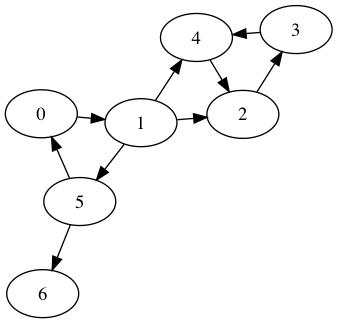
\includegraphics[width=\linewidth]{images/tarjan/0.png}
\caption{Initial graph.} \label{fig:tarjan0}
\end{subfigure}
\hspace*{\fill} % separation between the subfigures
\begin{subfigure}{0.3\textwidth}
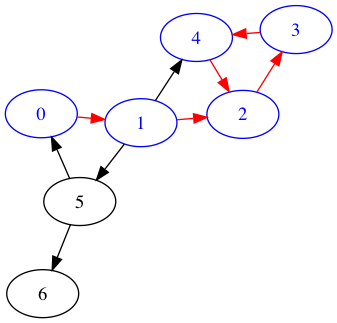
\includegraphics[width=\linewidth]{images/tarjan/1.png}
\caption{The search follows the path $0 \rightarrow 1 \rightarrow 2 \rightarrow 3 
\rightarrow 4 \rightarrow 2$.} \label{fig:tarjan1}
\end{subfigure}
\hspace*{\fill} % separation between the subfigures
\begin{subfigure}{0.3\textwidth}
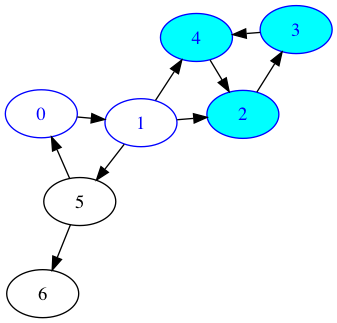
\includegraphics[width=\linewidth]{images/tarjan/2.png}
\caption{Since $lowlink[2] = 2$, nodes 2, 3 and 4 are added into a component.} \label{fig:tarjan2}
\end{subfigure}

\vspace{1cm}

\begin{subfigure}{0.3\textwidth}
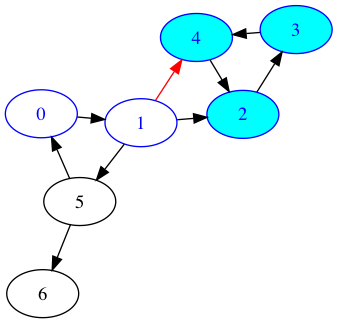
\includegraphics[width=\linewidth]{images/tarjan/3.png}
\caption{The search follows the path $1 \rightarrow 4$, but node $4$ has already been visited.} \label{fig:tarjan3}
\end{subfigure}
\hspace*{\fill} % separation between the subfigures
\begin{subfigure}{0.3\textwidth}
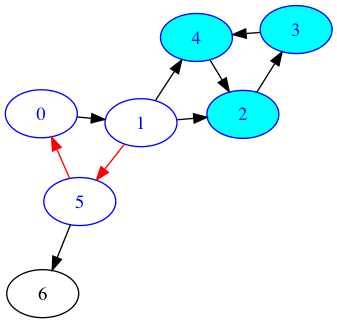
\includegraphics[width=\linewidth]{images/tarjan/4.png}
\caption{The search follows the path $1 \rightarrow 5 \rightarrow 0$.} \label{fig:tarjan6}
\end{subfigure}
\hspace*{\fill} % separation between the subfigures
\begin{subfigure}{0.3\textwidth}
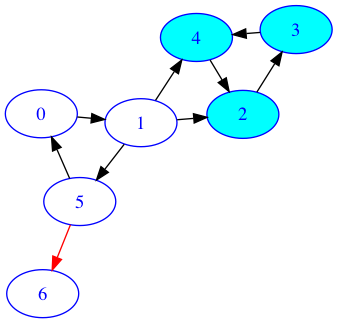
\includegraphics[width=\linewidth]{images/tarjan/5.png}
\caption{The search follows the path $5 \rightarrow 6$.} \label{fig:tarjan5}
\end{subfigure}

\vspace{1cm}

\begin{subfigure}{0.3\textwidth}
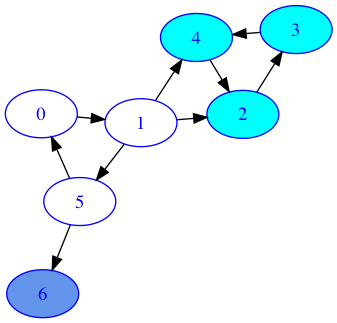
\includegraphics[width=\linewidth]{images/tarjan/6.png}
\caption{Node $6$ does not have outgoing edges and is added to a component.} \label{fig:tarjan6}
\end{subfigure}
\hspace*{2cm} % separation between the subfigures
\begin{subfigure}{0.3\textwidth}
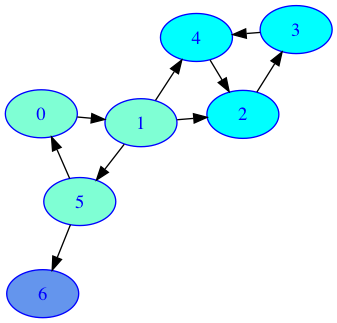
\includegraphics[width=\linewidth]{images/tarjan/7.png}
\caption{The algorithm returns to 0 and, since $lowlink[0] = 0$, adds 0, 1 and 5 to a component.} \label{fig:tarjan7}
\end{subfigure}


\caption{Example of an execution of Tarjan's strongly connected components algorithm.}\label{fig:tarjan}
\end{figure}

\autoref{fig:tarjan} illustrates the execution of Tarjan's algorithm.
The algorithm starts from node 0, with $index[0] = 0$ and $lowlink[0] = 0$.
With a depth-first search, the algorithm traces the path $0 \rightarrow 1 \rightarrow 2 \rightarrow 3 
\rightarrow 4 \rightarrow 2$.
Since node $2$ has already been visited and nodes 4 and 3 have no further outgoing edges, $lowlink[4]$ and $lowlink[3]$ receive the value 2 and the function calls return back to the first visit of node $2$.
At this point, nodes 2, 3 and 4 all have 2 as the smallest reachable index and, therefore, they form a strongly connected component.

Continuing from node 1, the algorithm traces $1 \rightarrow 5 \rightarrow 0$, but stops there since node 0 has already been visited.
Continuing from node 5, the algorithm traces $5 \rightarrow 7$.
Node 7 has no outgoing edges, so it forms a strongly connected component by itself.
Once the function calls return to node 0, a strongly connected component is formed with nodes 0, 1, and 5, since they all have 0 as their $lowlink$ value.

\section{Graph coloring with minimum colors}
\label{section:coloring}
%The algorithm proposed in \citep{mittal2011graph} is an efficient approach to graph coloring, a classic graph theory problem.
Graph coloring is one of the possible heuristics suggested by MaNI to detect malicious nodes after the generation of the component graph using Tarjan's algorithm.
Out of the tested heuristics, it presents the best results, so it has been chosen as the heuristic for TruMan.

The process of graph coloring consists of giving each node a label (represented by a color) so that no two neighboring nodes share the same color.
This problem has been studied in Computer Science since, at least, 1972 \citep{karp1972reducibility} and has been studied as a classic mathematics problem for even longer \citep{kempe1879geographical}.
It has been proven mathematically that any planar graph can be colored with at most four colors \citep{appel1976every}, but discovering the smallest number of colors necessary to color an arbitrary graph (called the graph's chromatic number) is an NP-hard problem \citep{sanchez1989determining}.

In \citep{mittal2011graph}, the authors present an efficient approach to graph coloring using the minimum possible amount of colors.
Although they do not prove that their algorithm always uses the smallest possible amount of colors, the output is always a correct coloration and the algorithm is nevertheless efficient.
For the purposes of trust management, it is not necessary to prove that the coloring algorithm's output uses the minimum possible number of colors.

The complexity of the algorithm is $O(|E'|)$ for a graph $C = (V',E')$.
As a comparison, the DSATUR algorithm for graph coloring has complexity $O(|V|^2)$ \citep{brelaz1979new}.
Algorithm \autoref{algorithm:coloring} shows the general structure of the graph coloring algorithm  \citep{mittal2011graph}.

\begin{algorithm}
\caption{Graph coloring with minimum colors}\label{algorithm:coloring}
\begin{algorithmic}[1]

\Function{Coloring}{graph $G$}

\State \textbf{color} all nodes of $G$ \textbf{with} 0
\State $d \rightarrow 0$
\For{$e=(u,v)$ \textbf{in} edges of $G$}
	\If{$u$ and $v$ have the same color}
		\If{$color[v] = d$}
			\State $d \rightarrow d+1$
		\EndIf
		\State $color[v] \rightarrow d$
	\EndIf
\EndFor


\EndFunction
\end{algorithmic}
\end{algorithm}


\begin{figure}
\centering

\begin{subfigure}{0.20\textwidth}
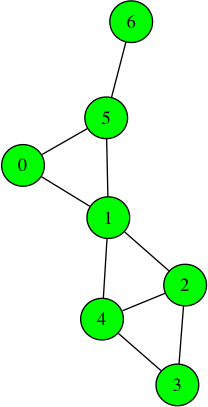
\includegraphics[width=\linewidth]{images/coloring/0.png}
\caption{Initial graph with all nodes labeled 1. $d=1$ (green).\\} \label{fig:coloring0}
\end{subfigure}
\hspace*{\fill} % separation between the subfigures
\begin{subfigure}{0.20\textwidth}
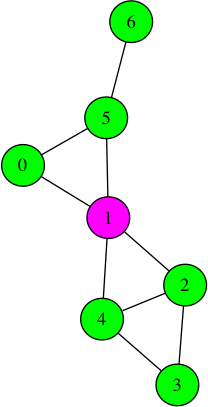
\includegraphics[width=\linewidth]{images/coloring/1.png}
\caption{Edge $(0,1)$ is checked and node $1$ gets a new color. $d=2$ (magenta).} \label{fig:coloring1}
\end{subfigure}
\hspace*{\fill} % separation between the subfigures
\begin{subfigure}{0.20\textwidth}
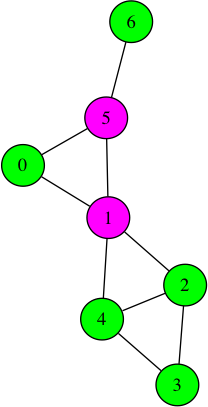
\includegraphics[width=\linewidth]{images/coloring/2.png}
\caption{Edge $(0,5)$ is checked and node $5$ gets the current value of $d$.} \label{fig:coloring2}
\end{subfigure}
\hspace*{\fill} % separation between the subfigures
\begin{subfigure}{0.20\textwidth}
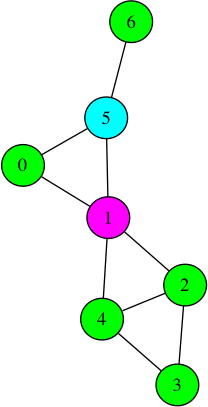
\includegraphics[width=\linewidth]{images/coloring/3.png}
\caption{Edge $(1,5)$ is checked and node $5$ gets a new color. $d=3$ (cyan).} \label{fig:coloring3}
\end{subfigure}

\vspace{2cm}

\begin{subfigure}{0.20\textwidth}
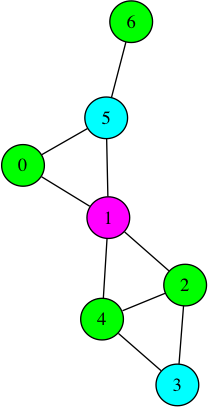
\includegraphics[width=\linewidth]{images/coloring/4.png}
\caption{Edge $(2,3)$ is checked and node $3$ gets the current value of $d$.} \label{fig:coloring5}
\end{subfigure}
\hspace*{2cm} % separation between the subfigures
\begin{subfigure}{0.20\textwidth}
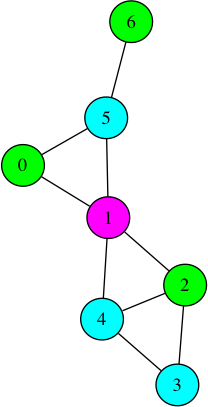
\includegraphics[width=\linewidth]{images/coloring/5.png}
\caption{Edge $(2,4)$ is checked and node $4$ gets the current value of $d$.} \label{fig:coloring6}
\end{subfigure}
\hspace*{2cm} % separation between the subfigures
\begin{subfigure}{0.20\textwidth}
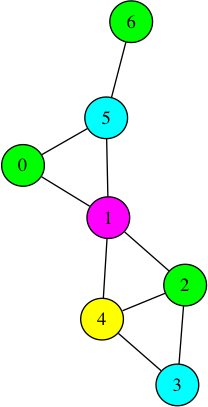
\includegraphics[width=\linewidth]{images/coloring/6.png}
\caption{Edge $(3,4)$ is checked and node $4$ gets a new color. $d=4$ (yellow).} \label{fig:coloring6}
\end{subfigure}

\caption{Example of an execution of the graph coloring with minimum colors algorithm.}\label{fig:coloring}
\end{figure}

A limitation of this algorithm is that the edges must be sorted according to node indexes.
It doesn't matter which nodes get assigned which indexes, but once they are assigned those numbers, the algorithm must follow the edges in numerical order.
This is demonstrated in \citep{vernize2013dissertation}.

\autoref{fig:coloring} illustrates the execution of the graph coloring algorithm.
It is notable how the algorithm takes few iterations to fully color the graph.
However, it is also possible to observe that the result does not use the minimum amount of colors.
By coloring node 4 as cyan and node 3 as magenta, the sample graph could have been colored with only three colors instead of four.
As described above, this is not a problem for the usage of the algorithm in TruMan.

\section{Malicious Node Identification Algorithm}

The basis of TruMan is the Malicious Node Identification Algorithm (MaNI) proposed in \citep{vernize2015malicious}, which suggests the use of strongly connected components and graph coloring for malicious node detection.
This article presents a malicious node identification scheme based on strongly connected components and graph coloring.
The model is proposed for complex networks in general, but is not suited for VANETs because it is designed only for static networks.
Furthermore, the algorithm is executed by a global observer which has information about the complete network.

The input graph $T = (V,E)$ is a static, connected, and directed graph containing all trust relationships in the network.
Such relationships are binary, so there are no varying degrees of trust: either one node trusts another completely (edge value is $1$), or it distrusts the other completely (edge value is $0$).
The relationships are also directed, meaning that if the value of $A\rightarrow B$ is $1$, $B\rightarrow A$ is not necessarily $1$.

The process for identifying malicious nodes within $T$ is as follows:

First, $T$ is separated into strongly connected components using Tarjan's algorithm \citep{tarjan1972depth}, which is described in detail in \autoref{section:tarjan}.
In each of these components, all nodes are connected by edges of value $1$.
In other words, within a single component, all nodes trust one another; nodes connected by edges of value $0$ are separated into different components.
Each of these components becomes a node of a component graph $C = (V', E')$.

The creation of the graph $C$ simplifies the remaining computation.
Since each node of $C$ is a vertex $v' \in V'$ and each vertex $v'$ is a component of $T$ in which all nodes trust each other, for the purposes of identifying malicious nodes, all nodes within each of those components can be treated as one.
They can either be benign nodes which legitimately trust one another, or malicious nodes colluding with each other.
After the formation of $C$, one or more heuristics can be used to classify the nodes as benign or malicious.

In the experiments performed by the authors of MaNI, the coloring heuristic shows the most promising results, identifying a high ratio of the malicious nodes in the network.
The coloring heuristic uses a graph coloring algorithm, such as DSATUR \citep{brelaz1979new} or the algorithm detailed in \autoref{section:coloring}.
Other heuristics were experimented with, but were either less effective in detecting malicious nodes, provided too many false positives, or were not efficient enough.

After running a graph coloring algorithm with graph $C$ as input, the color whose nodes in $C$ represent the most nodes in $T$ is classified as correct, and all others are classified as malicious.
Once this information from $C$ is brought back to graph $T$, it is trivial to label the nodes in $T$ as either benign or malicious based on their components' classifications.

Two types of experiments were made in each network: first, all malicious nodes inverted the edge weights leading to their neighbors; second, malicious nodes randomly inverted or not the weights.
In the first scenario, the results show excellent precision in most networks, detecting nearly every malicious node.
Experimenting with the second scenario, the results are less precise, however still promising: with up to 20\% of malicious nodes in the network, the error rate is under 7\%, while with the worst case, 50\% of the network being malicious, the error rate is approximately 15\%.

The authors suggest running the algorithm repeatedly after removing the malicious nodes from the network.
By doing this a small number of times, nearly all malicious nodes are detected by it even when randomly changing edge weights.

%\begin{algorithm}
%\caption{MaNI algorithm}\label{algorithm:mani}
%\begin{algorithmic}[1]
%
%\Function{MaNI}{graph $T$}
%
%\State $C \gets$ \textbf{Tarjan}$(T[0])$
%\State $colors \gets$ \textbf{Coloring}$(C)$
%\State \textbf{color} nodes of $T$ \textbf{according to} $colors$
%\State \textbf{count} 
%
%\EndFunction
%\end{algorithmic}
%\end{algorithm}

\begin{figure}
\centering

\begin{subfigure}{0.25\textwidth}
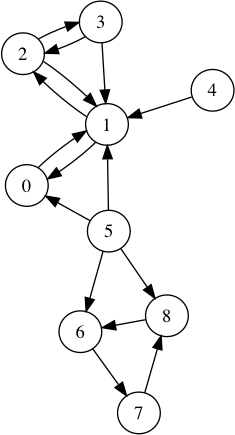
\includegraphics[width=\linewidth]{images/mani/0-trust.png}
\caption{Initial graph $T$.} \label{fig:mani0}
\end{subfigure}
\hspace*{2cm} % separation between the subfigures
\begin{subfigure}{0.25\textwidth}
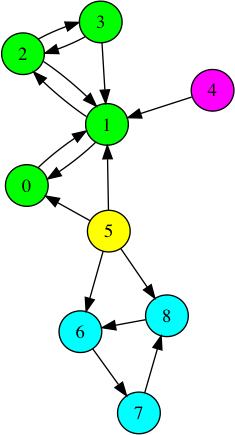
\includegraphics[width=\linewidth]{images/mani/1-tarjan.png}
\caption{Tarjan's algorithm is used to identify the strongly connected components.} \label{fig:mani1}
\end{subfigure}


\vspace{1cm} % separation between the subfigures

\begin{subfigure}{0.3\textwidth}
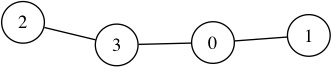
\includegraphics[width=\linewidth]{images/mani/2-components.png}
\caption{The graph $C$ is formed from the components of $T$.} \label{fig:mani2}
\end{subfigure}
\hspace*{2cm} % separation between the subfigures
\begin{subfigure}{0.3\textwidth}
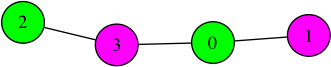
\includegraphics[width=\linewidth]{images/mani/3-colored-components.png}
\caption{The coloring algorithm is used to label the nodes of $C$.} \label{fig:mani3}
\end{subfigure}

\vspace{1cm} % separation between the subfigures

\begin{subfigure}{0.25\textwidth}
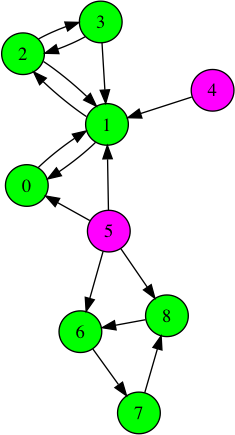
\includegraphics[width=\linewidth]{images/mani/4-result.png}
\caption{The colors from $C$ are used to label nodes in $T$ as correct or malicious.} \label{fig:mani4}
\end{subfigure}


\caption{Example of an execution of the MaNI algorithm.}\label{fig:mani}
\end{figure}


\autoref{fig:mani} illustrates the execution of the MaNI algorithm.
With the starting graph $T$, whose edges represent the trust relationships between nodes, Tarjan's strongly connected component algorithm is executed.
\autoref{fig:mani1} shows nodes colored according to their placement in a strongly connected component.
The strongly connected components form a graph $C$ according to edges present in $T$.
In \autoref{fig:mani2}, component $0$ is the one containing node $5$; component $1$ contains nodes $6$, $7$ and $8$; component $2$ contains nodes $0$, $1$, $2$ and $3$; and component $3$ contains node $4$.
The graph coloring with minimum colors algorithm is executed on $C$, producing the coloration shown in \autoref{fig:mani3}.
Finally, each node in $T$ is colored according to which color its component received in $C$.
The color with the most nodes is deemed benign, while the others are considered malicious. 


%$G = (V,E)$: undirected topology graph, in which $V$ are the vertices and $E$ are the edges.
%
%$T = (V,O)$: directed trust graph, in which $O$ are the nodes' opinions about each other.
%
%$G_t,T_t$: snapshots of $G$ and $T$ in a timestamp $t$.
%
%$G_i,T_i$: local knowledge of $G$ and $T$ of a node $i$.
%
%$C = (V',O')$: component graph of $T$.


\section{The TruMan algorithm}
\label{section:algorithm}

TruMan is based on the MaNI algorithm \citep{vernize2015malicious}, which suggested the use of Tarjan's algorithm and the graph coloring algorithm.
However, MaNI was developed for static networks such as social networks, and is executed by an external supervising agent (i.e. outside of the network), making it unsuitable for a vehicular network.

In order to work with dynamic networks, the TruMan algorithm runs iterations at predetermined intervals.
%As nodes acquire more information, their model of the network will change.
Furthermore, the algorithm runs in a decentralized fashion, meaning each node in the network runs its own instance of the algorithm.
Each node starts knowing information only about itself and maintains its own abstraction of the network surrounding it.
Every node $u$ stores a representation of the network in the form of a static, connected and directed trust graph $T^u = (V^u, E^u)$, in which $V^u$ is the set of nodes node $u$ is aware of and $E^u$ is the set of trust relationships (opinions) $u$ knows of between members of $V^u$.
Since each node has its own network representation and it changes over time, there is a $T^u_i = (V^u_i, E^u_i)$ for every node $u$ and iteration $i$.

At first, the node collects and organizes information.
A prerequisite of this step is a test that correctly classifies a neighboring node as benign or malicious.
There are several ways to perform such a test, but a study between these methods is beyond the scope of this paper.
Every time a neighboring node $v$ is tested as benign, the value of $u \rightarrow v$ increases.
Additionally, node $u$ performs an union between its trust graph and $v$'s trust graph, forming a new graph $T^u_i = T^u_{i-1} \bigcup T^v_{i-1}$, which is used for the remaining steps.

After the collection of data, $T^u_i$ is separated into strongly connected components using Tarjan's algorithm \citep{tarjan1972depth}, although the implementation of the algorithm slightly differs from the one used in MaNI.
Since MaNI uses binary trust, Tarjan's algorithm only checks whether edges have value 0 or 1; in TruMan, edges can have a range of values between 0 and 1.
Therefore, a threshold $h$ is defined so Tarjan's algorithm can consider only edges represent a significant trust relationship when forming strongly connected components.
So, for each node in a component, there is a path formed by edges of weight higher than the threshold $h$ to each other node in the same component.
Each of these components becomes a node of a component graph $C^u_i = (V'^u_i, E'^u_i)$.

Since each vertex $v' \in V'^u_i$ is a component of $T^u_i$ in which all nodes trust each other, for the purposes of identifying malicious nodes, all nodes within each of those components can be treated as the same.
They can either be benign nodes which legitimately trust one another, or malicious nodes colluding with each other.
After the formation of $C^u_i$, a heuristic is used to classify the nodes as benign or malicious.

The coloring heuristic is used to classify nodes, which uses the algorithm described in \autoref{section:coloring} \citep{mittal2011graph}, although other heuristics may be considered.
After running the graph coloring algorithm with graph $C^u_i$ as input, the color whose nodes in $C^u_i$ represent the most nodes in $T^u_i$ is classified as correct, and all others are classified as malicious.
Once this information from $C^u_i$ is brought back to graph $T^u_i$, it is trivial to label the nodes in $T^u_i$ as either benign or malicious based on the classifications of their components.

In summary, every node $u$ runs the following steps in each iteration to detect malicious nodes in the network:

\begin{enumerate}
	\item Node $u$ checks which are its neighbors (nodes within its communication range).
		  New discovered nodes and new formed edges are added to $T^u_i$.
		  Edges are created with weight 0.5.
	\item Node $u$ tests all its neighbors to discover which ones can be directly trusted or not.
		  New trust values are computed for the edges using the average between the previous value and either 1 (if the neighbor is trustworthy) or 0 (otherwise).
	\item If a neighbor $v$ is trustworthy, $u$ merges $T^v_{i-1}$ into $T^u_i$.
	\item Tarjan's algorithm is executed to identify the strongly connected components of $T^u_i$, resulting in a component graph $C^u_i$.
	\item The graph coloring algorithm is executed on $C^u_i$ and nodes are classified as benign or malicious.
\end{enumerate}

\subsection{Complexity}
The complexity of TruMan must calculated for each iteration executed and each node in the network.
It can be estimated by adding the complexity of most costly operations involved, which are: ($i$) Tarjan's algorithm, ($ii$) the graph coloring algorithm, and ($iii$) the graph union process.
Tarjan's algorithm and the graph coloring algorithm are executed once per iteration on each node of the network.
The graph union, however, is executed once every time a neighboring node shares information.
Each neighbor shares information once per iteration, so the complexity of the graph union procedure is multiplied by $n^u_i$, the number of neighbors node $u$ has during iteration $i$.

Therefore, the general complexity equation for each node and each iteration is as follows:

$$ TruMan = Tarjan + Coloring + (Union\times(n^u_i)) $$

As discussed above, Tarjan's algorithm has a complexity of $O(|V|+|E|)$ and is executed on graph $T$.
Meanwhile, the graph coloring algorithm has a complexity of $O(|E'|)$ and is executed on graph $C$.
The complexity of the graph merge algorithm is $O(|E|)$ and, in a worst-case scenario, $n^u_i$ is at most $|V|$ (every node in the network is a neighbor), resulting in a total complexity of $O(|V|\times |E|)$ for a whole iteration.
The total complexity of each iteration of TruMan is, therefore:

$$ O(|V|+|E|) + O(|E'|) + O(|V|\times |E|)$$

However, $|E'| \leq |E|$ is always true, because the graph $C$ is a reduction of graph $T$.
Furthermore, $|V|+|E| \leq |V|\times |E|$ is also true, except for the irrelevant scenarios of $|V| \leq 1$ or $|E| \leq 1$.

Therefore, the complexity can be simplified to: $O(|V| \times |E|)$.


%The MaNI algorithm works well and is efficient for static graphs.
%However, some important modifications had to be made to accommodate dynamic graphs.
%The main changes made are described below.
%
%\subsection{Graph knowledge and graph building}
%First of all, there is an important change to the graph knowledge used to run the algorithm.
%The complete trust graph is a parameter to the MaNI algorithm, which executes with complete knowledge of the graph.
%
%Given the complete topology graph $G = (V, E)$, each node $u \in V$ has its own vision of the network and $u$ has to build a graph, $G_u$, to represent its surrounding network.
%In each iteration of the algorithm, $u$ receives information from its neighbors about their own graphs.
%For every neighbor $v \in V$, $G_u$ must me merged with $G_v$.
%In sufficient iterations, $G_u$ forms a complete or nearly complete vision of the network.
%
%Alongside $G$, there is the trust graph $T = (V, O)$ which stores trust relationships between pairs of nodes in the form of directed edges.
%Again, each node $u$ has its own $T_u$, which contains the trust information node $u$ knows about.
%When a node $u$ asks for network information from node $v$, it also merges $T_u$ with $T_v$, but only if $u$ trusts $v$.
%If $u$ deems $v$ malicious, any information originating from $v$ cannot be considered valid.
%
%[Illustrate graph building here]
%
%Furthermore, this implies that the malicious node detection algorithm runs using incomplete graph knowledge.
%This is expected and generally unavoidable in vehicular networks, which have high mobility and can be extremely large.
%
%
%
%-\\
%----------\\
%This paragraph is probably pertinent to delimiting the size of graphs:\\
%The authors of \citep{patwardhan2006data} provide important observations regarding the collection of data from local conditions.
%Most crucially, they mention how the quality of information is higher when the origin of such information is close to the destination node.
%That is, data collected by the node's own sensors have the highest quality, which diminishes as information starts to come from neighbors, neighbors of neighbors and so forth.
%They adopt a broadcast model in which RSUs send data about its surroundings and OBUs capture the information.
%The trust model proposed here might use a similar broadcast model, although adapted so all nodes are vehicles (OBUs).\\
%----------\\

%The original work's scope does not include the generation of the trust graph, as it is a parameter to the algorithm.
%In dynamic graphs, trust relationships change over time, so how those changes affect the proposed trust model have to be considered.
%This includes not only the full figure of the graph, but also each node's views on its neighbors.
%
%\subsection{Strongly connected components}
%Strongly connected components, or components in which all nodes have positive trust relationships with each other, are somewhat different in dynamic graphs.
%As nodes enter, leave, or change locations in the network, the components change accordingly.
%Therefore, our algorithm will have to work using ``snapshots'' of the graph, meaning each measurement will be valid for a specific timestamp.
%Since the graph changes with time, for every timestamp $t$, there is a corresponding topology graph $G_t=(V_t, E_t)$, which includes the available vertices and edges in that moment in time, and a trust graph $T_t=(V_t, O_t)$, with the nodes' opinions at that moment.
%
%In a later step, it might be useful to consider how specific nodes may change over several snapshots.
%Specifically, the suggestion of running the algorithm in iterations, by removing the malicious nodes in each step, may be applied with the peculiarities of a dynamic network.
%
%\subsection{Graph knowledge}
%In the original paper, the malicious nodes are identified by a central entity with access to all nodes' trust values.
%Not only does our work plan to decentralize this procedure, having complete knowledge of the graph is unfeasible in large-scale dynamic networks such as VANETs.
%Therefore, our algorithm needs to work using only a partial understanding of the network.
%For this to be viable, each node might have to gather information not only from its views on its neighbors, but also from its neighbors' views.
%
%The authors of \citep{patwardhan2006data} provide important observations regarding the collection of data from local conditions.
%Most crucially, they mention how the quality of information is higher when the origin of such information is close to the destination node.
%That is, data collected by the node's own sensors have the highest quality, which diminishes as information starts to come from neighbors, neighbors of neighbors and so forth.
%They adopt a broadcast model in which RSUs send data about its surroundings and OBUs capture the information.
%The trust model proposed here might use a similar broadcast model, although adapted so all nodes are vehicles (OBUs).
%
%Thus, each node has its own model of the network topology, $G_i$, and generates a trust graph $T_i=(V_i, O_i)$, in which $i$ is the node's identifier.
%Combined with the necessity of timestamps explained above, this results in a graph $T_{it}=(V_{it}, O_{it})$ for each node and each timestamp, which is the input of the new algorithm.
%Accordingly, there are also component graphs $C_{it}=(V'_{it}, O'_{it})$, generated on each instance of the algorithm.
%
%During the early stages of development, it will be considered that vertices cannot enter or leave the network and, therefore, only the layout of the edges changes.
%This is sufficient to experiment with the algorithm's performance with the added complexity of a dynamic network.
%
%
%\subsection{Binary trust}
%A model using binary trust is one in which trust values can only be 0 or 1.
%If node $A$ positively trusts node $B$, the value of the edge $A\rightarrow B$ is 1.
%If it does not trust $B$, or is unsure, the value is 0.
%Such a scheme makes sense in a static graph but, in a dynamic one, it is interesting to have a range of possible trust values.
%
%Since nodes interact with each other occasionally and might learn information from other nodes, a range of $[0,1]$ is useful to express how one trust value can change over time.
%As one node learns more about another, the value can grow or diminish and, once it goes above or below a certain threshold, the neighboring node can be deemed trustworthy or not.
%The rate in which trust increases or decreases must be experimented with; it could be useful to have trust decrease faster than it increases, but that might also cause false positives in the case of occasional mistakes.
%
%\subsection{Datasets}
%The datasets used for experimentation must be changed accordingly.
%Instead of using data gathered from social networks, which are static, dynamic network datasets must be used, such as traffic information for cities.
%
%At first, the objective is to test using the Working Day Movement Model, setting parameters that contribute to the validation of the algorithm.
%When the simulation begins, a set number of nodes are malicious and, therefore, other nodes will have low trust in them after interacting.
%In time, benign and malicious nodes can change their behavior and, accordingly, their trustworthiness will be updated.
%
%It might still be useful to simulate using real-world movement traces.
%An example of such dataset is the Zurich Trace \citep{zurichtrace}, which describes the vehicular traces in the city of Zurich, Switzerland.
%The chosen dataset doesn't necessarily need to be created for VANETs, since with vehicular traces it is possible to assume all or a percentage of the traced vehicles are smart and can be nodes of a hypothetical VANET.
%The mobility of the nodes is the most important aspect of the dataset.		% 
\chapter{TruMan}
\label{chap:truman}

%This work shows that it is possible to adapt a trust management scheme originally designed for static networks to a dynamic environment, such as a VANET.
This work introduces an efficient solution to trust management in dynamic networks such as VANETs.
In order to make this possible, it is necessary to identify features in VANETs that show that nodes can share a long-term relationship, as is the case for social networks.
%The arguments for such features are presented in \autoref{section:socialvanets}, while the movement model that enables the simulation of the features is explained in \autoref{section:workingday}.
Through these long-term relationships, it then becomes feasible for nodes to store trust data and share it with other nodes.
By combining a node's own opinions about familiar nodes and trust information received from its neighbors, it is possible to create a model of the surrounding network.
This model includes a trust graph, showing the trust relationships between pair of nodes, which can then be used in conjunction with other algorithms in order to classify nodes as correct or malicious.

%The previous chapters show why vehicular networks require distinguished trust models compared to social networks and traditional MANETs.
%In this chapter, it is proposed that certain aspects from social networks can be found in vehicular networks and, through those aspects, it is possible to adapt a trust model designed for traditional complex networks to a vehicular environment.
%These social properties allow for long-term trust relationships to be established amongst nodes of a network and, therefore, previously existing trust models can be adapted to the vehicular environment.

In this chapter, the reasoning behind TruMan and details of how it works are presented.
First, it is shown how vehicles can form long-term relationships and trust one another in a similar way to social networks.
Then, two algorithms are introduced: Tarjan's strongly connected components algorithm \citep{tarjan1972depth} and an efficient algorithm for graph coloring \citep{mittal2011graph}.
Next, the Malicious Node Identification Algorithm (MaNI) \citep{vernize2013dissertation} is explained, because it is the work that suggests the usage of strongly connected components and graph coloring for malicious node detection.
Finally, TruMan itself is detailed, showing how it combines features from existing algorithms and adapts them to a dynamic environment, enabled by the social properties found in vehicular networks.
%Then, the Working Day Movement Model is introduced, along with the reasons why it is best fitted for this work.
%Next, a previously existing trust model for complex networks is described, including its advantages and reasons why it could be well-fitted for a vehicular environment, followed by a list of changes that must be made to the model in order for it to handle dynamic networks.
%Finally, a schedule for the next steps of the project is shown.

\section{Goals}
\label{section:goals}
Building from the foundation set by MaNI \citep{vernize2013dissertation}, TruMan strives to enable efficient trust management in highly dynamic networks such as VANETs.
In addition to efficiency, it is desirable that the trust model is both simple to understand and to implement, making it appealing for real-world usage.

Furthermore, the desired properties of a VANET trust model described in \citep{zhang2011survey} (explained in detail in \autoref{section:properties}) were considered, so TruMan attempts to fulfill or enable as many of those properties as possible.

\section{Social Networks and VANETs}
\label{section:socialvanets}
Some proposed trust models for vehicular networks, such as \citep{huang2014social}, state that the likelihood of two nodes meeting each other twice is too low to be relevant.
However, it stands to reason that, throughout the course of several days, many drivers take similar routes at similar times of day (e.g. to commute to work) and, therefore, their vehicles are in similar locations each day.
Additionally, many cities rely on main roads to serve as backbones to their traffic, meaning there is a high density of vehicles on those roads during rush hours.
Since that is true for a notable percentage of a city's fleet, it can also be assumed that those vehicles may frequently encounter each other during their commute.
While two vehicles that share a commute route may not be direct neighbors every day, they are likely to be relatively close to each other most days, meaning few hops separate them in the ad-hoc network.
Furthermore, certain pairs of vehicles are bound to be within communication range of each other nearly every day.
Examples of these include vehicles whose owners are neighbors or coworkers.
Such vehicles' trust relationship should become steady over time and, in the case of positive trust, they can use each other's information to learn more about other nodes in the network.

%\textbf{[WORKING DAY MOBILITY MODEL]}
%They do not, however, present data regarding specific pairs of nodes.
%[Should we propose to show this information in our work?]

%Regardless of these properties of commuting vehicles, the probability of two specific vehicles meeting each other more than once, in given time, tends to 1.
%So it is also reasonable to assume that two vehicles, whose drivers reside in the same city, over a long period of time (e.g. one year) may meet each other more than once.
%However, if they only meet rarely, their trust opinions about each other may not be very useful.

Most cities also have one or more types of mass transit systems (buses or trains).
Those vehicles can also be part of a VANET and communicate with private cars.
Buses share the same roads as cars, but instead of having specific destinations, they travel a predefined route during the whole day, usually tied to a tight schedule.
Trains travel on rails, so their contact with cars is less frequent, but it can also happen on railroad crossings; they travel long distances in relatively short amount of time, which helps the dissemination of data in a VANET.
In the same way that cars have a high probability of meeting more than once during their commutes, it is also very likely that they meet the same buses and/or trains frequently.

In \citep{da2013effective}, \citep{cunha2014vehicular}, and \citep{cunha2014possible}, the authors attempt to find features usually attributed to social networks in vehicular networks.
By using a data set from the city of Zurich, Switzerland, they show that some metrics, such as clustering coefficient and number of encounters, have peaks during the rush hours.
They note that, during rush hours, the diameter of the graph decreases to around 6 hops; additionally, the frequency of total encounters between pairs of nodes in the network increases during those hours.
Although the authors do not quantify the encounters between specific pairs of nodes, these numbers support the idea that daily commutes do indeed cause vehicular networks to exhibit social network features.

%Another way of applying trust models from social networks to VANETs would be to take into account the relationships between drivers.
%If a neighboring vehicle happens to be driven by a close friend or relative, there is reason to believe that it is not a malicious node in the network.
%That might not always be the case, since there may be malicious hackers controlling the node and its driver is oblivious to it.
%In any case, this approach is not covered in this work.


\section{Tarjan's strongly connected components algorithm}
\label{section:tarjan}
The use of Tarjan's strongly connected components algorithm \citep{tarjan1972depth} is an important aspect of TruMan's efficiency.
This allows a large graph to be abstracted into a smaller one, which therefore reduces the input for further steps.
Given a directed graph $T = (V,E)$, a strongly connected component is defined as a group of nodes in which, for any pair of nodes $u, v \in V$, there is a path from $u$ to $v$ and a path from $v$ to $u$.
For the purposes of trust management, this definition is extended to accept only paths of edges with weight above a predetermined threshold $h$.
Every node of the input graph $T$ must belong to a component.

The algorithm works by performing a depth-first search, adding nodes to a stack as they are visited.
If two nodes are present on the stack, then there is a path from the first node to the second one (in the order they were added to the stack).

Each node has two attributes assigned to it during the execution of the algorithm: $index$ is used to number the nodes in the order they are visited, while $lowlink$ is the lowest indexed node reachable from each node.
In the implementation used, $index$, $lowlink$, $count$ and $stack$ are global variables accessed from every call of the function.
$index$ and $lowlink$ are arrays indexed by unique node identifiers, $count$ is an integer and $stack$ is a last-in-first-out data structure.

In the call that visits a node $u$, the algorithm must loop through each node $v$ trusted by $u$ (that is, $u \rightarrow v$ exists and has value greater than $h$).
If node $v$ has not yet been visited, the algorithm is called for $v$.
The $lowlink$ of $u$ is then calculated as the smallest value between $lowlink[u]$ and $lowlink[v]$, because any node reachable from $v$ is also reachable from $u$.
After the loop, if $lowlink[u]$ is equal to $index[u]$, it means that $u$ is the lowest indexed node reachable from itself and that it is the root of a component.
Therefore, nodes must be popped from the stack until $u$ is found.
Each node popped, including $u$, is a member of a strongly connected component.

The number of components is, at most, $|V|$: in a worst-case scenario, each node is placed into its own component.
The complexity of the algorithm is $O(|V|+|E|)$ for a graph $T = (V,E)$.
Algorithm \autoref{algorithm:tarjan} shows the general structure of Tarjan's algorithm  \citep{tarjan1972depth}.

\begin{algorithm}
\caption{Tarjan's strongly connected components algorithm}\label{algorithm:tarjan}
\begin{algorithmic}[1]

\Function{Tarjan}{vertex $u$}

\State $index[u] = count$
\State $lowlink[u] = count$
\State $count \gets count + 1$
\State \textbf{push} $u$ \textbf{to} $stack$

\For{$v$ \textbf{in} neighbors of $u$ }

	\If{weight of $u\rightarrow v < h$}
		\State \textbf{continue}
	\EndIf
	
	\If{$index[v] = -1$}
		\Comment{\emph{v has not been visited yet}}
		\State \textbf{Tarjan}($v$)
	\EndIf
	
	\State $lowlink[u] \gets \textbf{min}(lowlink[u],lowlink[v])$
\EndFor

\If{$lowlink[u] = index[u]$}
	\Repeat
		\Comment{\emph{unstack nodes until u is found}}
		\State \textbf{pop} $w$ \textbf{from} $stack$
		\State \textbf{add} $w$ \textbf{to} $component$
	\Until {$w = u$}
\EndIf

\EndFunction
\end{algorithmic}
\end{algorithm}


\begin{figure}
\centering

\begin{subfigure}{0.30\textwidth}
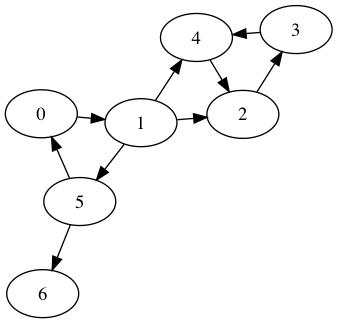
\includegraphics[width=\linewidth]{images/tarjan/0.png}
\caption{Initial graph.} \label{fig:tarjan0}
\end{subfigure}
\hspace*{\fill} % separation between the subfigures
\begin{subfigure}{0.3\textwidth}
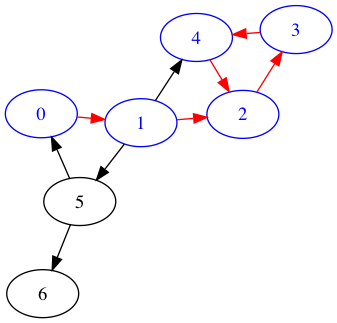
\includegraphics[width=\linewidth]{images/tarjan/1.png}
\caption{The search follows the path $0 \rightarrow 1 \rightarrow 2 \rightarrow 3 
\rightarrow 4 \rightarrow 2$.} \label{fig:tarjan1}
\end{subfigure}
\hspace*{\fill} % separation between the subfigures
\begin{subfigure}{0.3\textwidth}
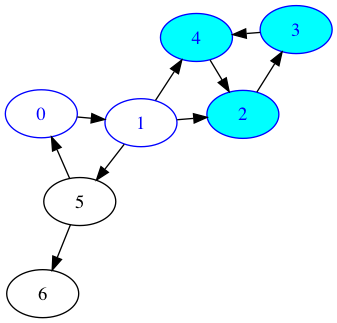
\includegraphics[width=\linewidth]{images/tarjan/2.png}
\caption{Since $lowlink[2] = 2$, nodes 2, 3 and 4 are added into a component.} \label{fig:tarjan2}
\end{subfigure}

\vspace{1cm}

\begin{subfigure}{0.3\textwidth}
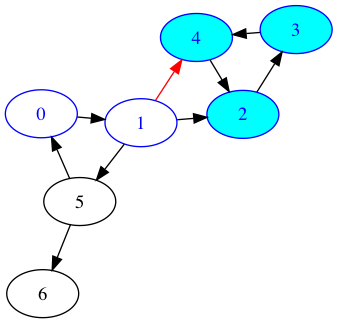
\includegraphics[width=\linewidth]{images/tarjan/3.png}
\caption{The search follows the path $1 \rightarrow 4$, but node $4$ has already been visited.} \label{fig:tarjan3}
\end{subfigure}
\hspace*{\fill} % separation between the subfigures
\begin{subfigure}{0.3\textwidth}
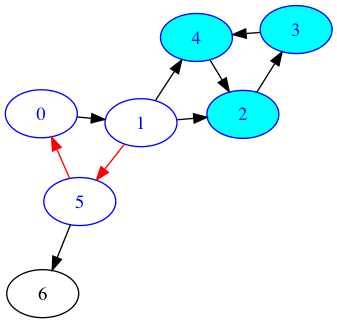
\includegraphics[width=\linewidth]{images/tarjan/4.png}
\caption{The search follows the path $1 \rightarrow 5 \rightarrow 0$.} \label{fig:tarjan6}
\end{subfigure}
\hspace*{\fill} % separation between the subfigures
\begin{subfigure}{0.3\textwidth}
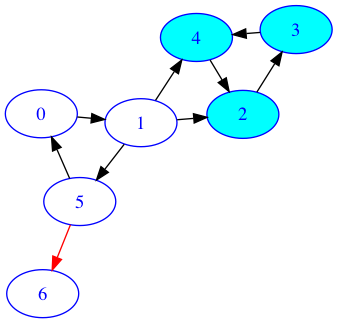
\includegraphics[width=\linewidth]{images/tarjan/5.png}
\caption{The search follows the path $5 \rightarrow 6$.} \label{fig:tarjan5}
\end{subfigure}

\vspace{1cm}

\begin{subfigure}{0.3\textwidth}
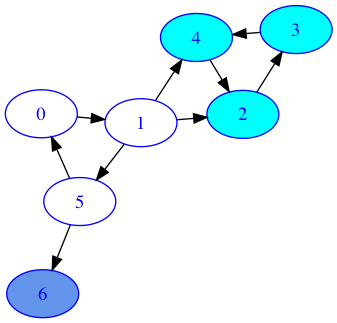
\includegraphics[width=\linewidth]{images/tarjan/6.png}
\caption{Node $6$ does not have outgoing edges and is added to a component.} \label{fig:tarjan6}
\end{subfigure}
\hspace*{2cm} % separation between the subfigures
\begin{subfigure}{0.3\textwidth}
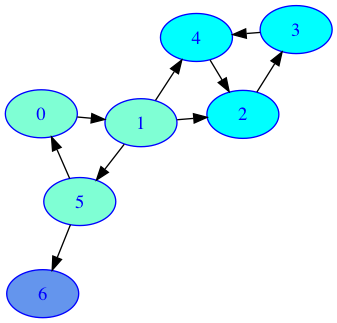
\includegraphics[width=\linewidth]{images/tarjan/7.png}
\caption{The algorithm returns to 0 and, since $lowlink[0] = 0$, adds 0, 1 and 5 to a component.} \label{fig:tarjan7}
\end{subfigure}


\caption{Example of an execution of Tarjan's strongly connected components algorithm.}\label{fig:tarjan}
\end{figure}

\autoref{fig:tarjan} illustrates the execution of Tarjan's algorithm.
The algorithm starts from node 0, with $index[0] = 0$ and $lowlink[0] = 0$.
With a depth-first search, the algorithm traces the path $0 \rightarrow 1 \rightarrow 2 \rightarrow 3 
\rightarrow 4 \rightarrow 2$.
Since node $2$ has already been visited and nodes 4 and 3 have no further outgoing edges, $lowlink[4]$ and $lowlink[3]$ receive the value 2 and the function calls return back to the first visit of node $2$.
At this point, nodes 2, 3 and 4 all have 2 as the smallest reachable index and, therefore, they form a strongly connected component.

Continuing from node 1, the algorithm traces $1 \rightarrow 5 \rightarrow 0$, but stops there since node 0 has already been visited.
Continuing from node 5, the algorithm traces $5 \rightarrow 7$.
Node 7 has no outgoing edges, so it forms a strongly connected component by itself.
Once the function calls return to node 0, a strongly connected component is formed with nodes 0, 1, and 5, since they all have 0 as their $lowlink$ value.

\section{Graph coloring with minimum colors}
\label{section:coloring}
%The algorithm proposed in \citep{mittal2011graph} is an efficient approach to graph coloring, a classic graph theory problem.
Graph coloring is one of the possible heuristics suggested by MaNI to detect malicious nodes after the generation of the component graph using Tarjan's algorithm.
Out of the tested heuristics, it presents the best results, so it has been chosen as the heuristic for TruMan.

The process of graph coloring consists of giving each node a label (represented by a color) so that no two neighboring nodes share the same color.
This problem has been studied in Computer Science since, at least, 1972 \citep{karp1972reducibility} and has been studied as a classic mathematics problem for even longer \citep{kempe1879geographical}.
It has been proven mathematically that any planar graph can be colored with at most four colors \citep{appel1976every}, but discovering the smallest number of colors necessary to color an arbitrary graph (called the graph's chromatic number) is an NP-hard problem \citep{sanchez1989determining}.

In \citep{mittal2011graph}, the authors present an efficient approach to graph coloring using the minimum possible amount of colors.
Although they do not prove that their algorithm always uses the smallest possible amount of colors, the output is always a correct coloration and the algorithm is nevertheless efficient.
For the purposes of trust management, it is not necessary to prove that the coloring algorithm's output uses the minimum possible number of colors.

The complexity of the algorithm is $O(|E'|)$ for a graph $C = (V',E')$.
As a comparison, the DSATUR algorithm for graph coloring has complexity $O(|V|^2)$ \citep{brelaz1979new}.
Algorithm \autoref{algorithm:coloring} shows the general structure of the graph coloring algorithm  \citep{mittal2011graph}.

\begin{algorithm}
\caption{Graph coloring with minimum colors}\label{algorithm:coloring}
\begin{algorithmic}[1]

\Function{Coloring}{graph $G$}

\State \textbf{color} all nodes of $G$ \textbf{with} 0
\State $d \rightarrow 0$
\For{$e=(u,v)$ \textbf{in} edges of $G$}
	\If{$u$ and $v$ have the same color}
		\If{$color[v] = d$}
			\State $d \rightarrow d+1$
		\EndIf
		\State $color[v] \rightarrow d$
	\EndIf
\EndFor


\EndFunction
\end{algorithmic}
\end{algorithm}


\begin{figure}
\centering

\begin{subfigure}{0.20\textwidth}
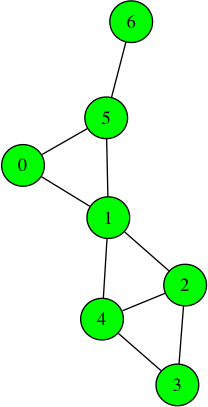
\includegraphics[width=\linewidth]{images/coloring/0.png}
\caption{Initial graph with all nodes labeled 1. $d=1$ (green).\\} \label{fig:coloring0}
\end{subfigure}
\hspace*{\fill} % separation between the subfigures
\begin{subfigure}{0.20\textwidth}
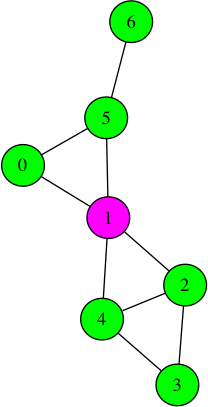
\includegraphics[width=\linewidth]{images/coloring/1.png}
\caption{Edge $(0,1)$ is checked and node $1$ gets a new color. $d=2$ (magenta).} \label{fig:coloring1}
\end{subfigure}
\hspace*{\fill} % separation between the subfigures
\begin{subfigure}{0.20\textwidth}
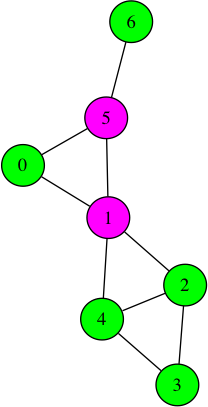
\includegraphics[width=\linewidth]{images/coloring/2.png}
\caption{Edge $(0,5)$ is checked and node $5$ gets the current value of $d$.} \label{fig:coloring2}
\end{subfigure}
\hspace*{\fill} % separation between the subfigures
\begin{subfigure}{0.20\textwidth}
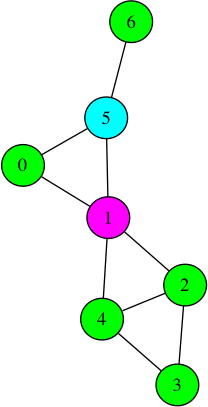
\includegraphics[width=\linewidth]{images/coloring/3.png}
\caption{Edge $(1,5)$ is checked and node $5$ gets a new color. $d=3$ (cyan).} \label{fig:coloring3}
\end{subfigure}

\vspace{2cm}

\begin{subfigure}{0.20\textwidth}
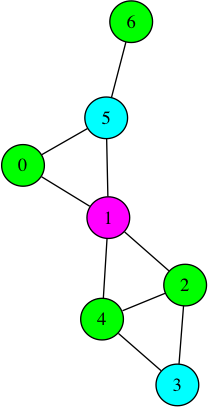
\includegraphics[width=\linewidth]{images/coloring/4.png}
\caption{Edge $(2,3)$ is checked and node $3$ gets the current value of $d$.} \label{fig:coloring5}
\end{subfigure}
\hspace*{2cm} % separation between the subfigures
\begin{subfigure}{0.20\textwidth}
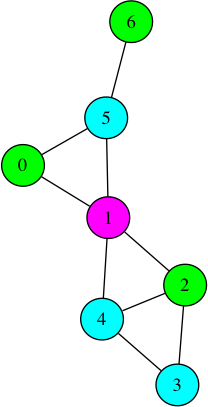
\includegraphics[width=\linewidth]{images/coloring/5.png}
\caption{Edge $(2,4)$ is checked and node $4$ gets the current value of $d$.} \label{fig:coloring6}
\end{subfigure}
\hspace*{2cm} % separation between the subfigures
\begin{subfigure}{0.20\textwidth}
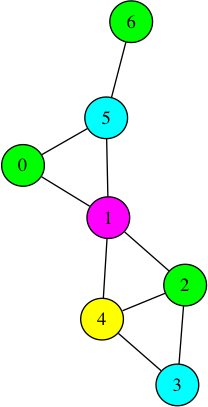
\includegraphics[width=\linewidth]{images/coloring/6.png}
\caption{Edge $(3,4)$ is checked and node $4$ gets a new color. $d=4$ (yellow).} \label{fig:coloring6}
\end{subfigure}

\caption{Example of an execution of the graph coloring with minimum colors algorithm.}\label{fig:coloring}
\end{figure}

A limitation of this algorithm is that the edges must be sorted according to node indexes.
It doesn't matter which nodes get assigned which indexes, but once they are assigned those numbers, the algorithm must follow the edges in numerical order.
This is demonstrated in \citep{vernize2013dissertation}.

\autoref{fig:coloring} illustrates the execution of the graph coloring algorithm.
It is notable how the algorithm takes few iterations to fully color the graph.
However, it is also possible to observe that the result does not use the minimum amount of colors.
By coloring node 4 as cyan and node 3 as magenta, the sample graph could have been colored with only three colors instead of four.
As described above, this is not a problem for the usage of the algorithm in TruMan.

\section{Malicious Node Identification Algorithm}

The basis of TruMan is the Malicious Node Identification Algorithm (MaNI) proposed in \citep{vernize2015malicious}, which suggests the use of strongly connected components and graph coloring for malicious node detection.
This article presents a malicious node identification scheme based on strongly connected components and graph coloring.
The model is proposed for complex networks in general, but is not suited for VANETs because it is designed only for static networks.
Furthermore, the algorithm is executed by a global observer which has information about the complete network.

The input graph $T = (V,E)$ is a static, connected, and directed graph containing all trust relationships in the network.
Such relationships are binary, so there are no varying degrees of trust: either one node trusts another completely (edge value is $1$), or it distrusts the other completely (edge value is $0$).
The relationships are also directed, meaning that if the value of $A\rightarrow B$ is $1$, $B\rightarrow A$ is not necessarily $1$.

The process for identifying malicious nodes within $T$ is as follows:

First, $T$ is separated into strongly connected components using Tarjan's algorithm \citep{tarjan1972depth}, which is described in detail in \autoref{section:tarjan}.
In each of these components, all nodes are connected by edges of value $1$.
In other words, within a single component, all nodes trust one another; nodes connected by edges of value $0$ are separated into different components.
Each of these components becomes a node of a component graph $C = (V', E')$.

The creation of the graph $C$ simplifies the remaining computation.
Since each node of $C$ is a vertex $v' \in V'$ and each vertex $v'$ is a component of $T$ in which all nodes trust each other, for the purposes of identifying malicious nodes, all nodes within each of those components can be treated as one.
They can either be benign nodes which legitimately trust one another, or malicious nodes colluding with each other.
After the formation of $C$, one or more heuristics can be used to classify the nodes as benign or malicious.

In the experiments performed by the authors of MaNI, the coloring heuristic shows the most promising results, identifying a high ratio of the malicious nodes in the network.
The coloring heuristic uses a graph coloring algorithm, such as DSATUR \citep{brelaz1979new} or the algorithm detailed in \autoref{section:coloring}.
Other heuristics were experimented with, but were either less effective in detecting malicious nodes, provided too many false positives, or were not efficient enough.

After running a graph coloring algorithm with graph $C$ as input, the color whose nodes in $C$ represent the most nodes in $T$ is classified as correct, and all others are classified as malicious.
Once this information from $C$ is brought back to graph $T$, it is trivial to label the nodes in $T$ as either benign or malicious based on their components' classifications.

Two types of experiments were made in each network: first, all malicious nodes inverted the edge weights leading to their neighbors; second, malicious nodes randomly inverted or not the weights.
In the first scenario, the results show excellent precision in most networks, detecting nearly every malicious node.
Experimenting with the second scenario, the results are less precise, however still promising: with up to 20\% of malicious nodes in the network, the error rate is under 7\%, while with the worst case, 50\% of the network being malicious, the error rate is approximately 15\%.

The authors suggest running the algorithm repeatedly after removing the malicious nodes from the network.
By doing this a small number of times, nearly all malicious nodes are detected by it even when randomly changing edge weights.

%\begin{algorithm}
%\caption{MaNI algorithm}\label{algorithm:mani}
%\begin{algorithmic}[1]
%
%\Function{MaNI}{graph $T$}
%
%\State $C \gets$ \textbf{Tarjan}$(T[0])$
%\State $colors \gets$ \textbf{Coloring}$(C)$
%\State \textbf{color} nodes of $T$ \textbf{according to} $colors$
%\State \textbf{count} 
%
%\EndFunction
%\end{algorithmic}
%\end{algorithm}

\begin{figure}
\centering

\begin{subfigure}{0.25\textwidth}
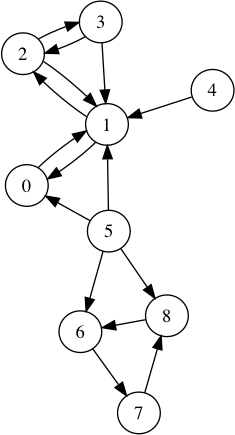
\includegraphics[width=\linewidth]{images/mani/0-trust.png}
\caption{Initial graph $T$.} \label{fig:mani0}
\end{subfigure}
\hspace*{2cm} % separation between the subfigures
\begin{subfigure}{0.25\textwidth}
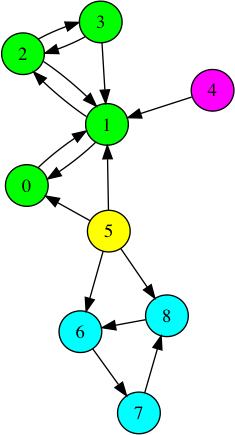
\includegraphics[width=\linewidth]{images/mani/1-tarjan.png}
\caption{Tarjan's algorithm is used to identify the strongly connected components.} \label{fig:mani1}
\end{subfigure}


\vspace{1cm} % separation between the subfigures

\begin{subfigure}{0.3\textwidth}
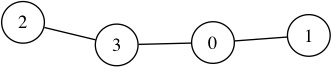
\includegraphics[width=\linewidth]{images/mani/2-components.png}
\caption{The graph $C$ is formed from the components of $T$.} \label{fig:mani2}
\end{subfigure}
\hspace*{2cm} % separation between the subfigures
\begin{subfigure}{0.3\textwidth}
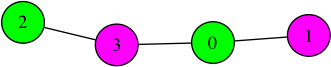
\includegraphics[width=\linewidth]{images/mani/3-colored-components.png}
\caption{The coloring algorithm is used to label the nodes of $C$.} \label{fig:mani3}
\end{subfigure}

\vspace{1cm} % separation between the subfigures

\begin{subfigure}{0.25\textwidth}
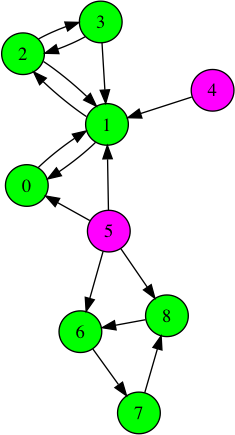
\includegraphics[width=\linewidth]{images/mani/4-result.png}
\caption{The colors from $C$ are used to label nodes in $T$ as correct or malicious.} \label{fig:mani4}
\end{subfigure}


\caption{Example of an execution of the MaNI algorithm.}\label{fig:mani}
\end{figure}


\autoref{fig:mani} illustrates the execution of the MaNI algorithm.
With the starting graph $T$, whose edges represent the trust relationships between nodes, Tarjan's strongly connected component algorithm is executed.
\autoref{fig:mani1} shows nodes colored according to their placement in a strongly connected component.
The strongly connected components form a graph $C$ according to edges present in $T$.
In \autoref{fig:mani2}, component $0$ is the one containing node $5$; component $1$ contains nodes $6$, $7$ and $8$; component $2$ contains nodes $0$, $1$, $2$ and $3$; and component $3$ contains node $4$.
The graph coloring with minimum colors algorithm is executed on $C$, producing the coloration shown in \autoref{fig:mani3}.
Finally, each node in $T$ is colored according to which color its component received in $C$.
The color with the most nodes is deemed benign, while the others are considered malicious. 


%$G = (V,E)$: undirected topology graph, in which $V$ are the vertices and $E$ are the edges.
%
%$T = (V,O)$: directed trust graph, in which $O$ are the nodes' opinions about each other.
%
%$G_t,T_t$: snapshots of $G$ and $T$ in a timestamp $t$.
%
%$G_i,T_i$: local knowledge of $G$ and $T$ of a node $i$.
%
%$C = (V',O')$: component graph of $T$.


\section{The TruMan algorithm}
\label{section:algorithm}

TruMan is based on the MaNI algorithm \citep{vernize2015malicious}, which suggested the use of Tarjan's algorithm and the graph coloring algorithm.
However, MaNI was developed for static networks such as social networks, and is executed by an external supervising agent (i.e. outside of the network), making it unsuitable for a vehicular network.

In order to work with dynamic networks, the TruMan algorithm runs iterations at predetermined intervals.
%As nodes acquire more information, their model of the network will change.
Furthermore, the algorithm runs in a decentralized fashion, meaning each node in the network runs its own instance of the algorithm.
Each node starts knowing information only about itself and maintains its own abstraction of the network surrounding it.
Every node $u$ stores a representation of the network in the form of a static, connected and directed trust graph $T^u = (V^u, E^u)$, in which $V^u$ is the set of nodes node $u$ is aware of and $E^u$ is the set of trust relationships (opinions) $u$ knows of between members of $V^u$.
Since each node has its own network representation and it changes over time, there is a $T^u_i = (V^u_i, E^u_i)$ for every node $u$ and iteration $i$.

At first, the node collects and organizes information.
A prerequisite of this step is a test that correctly classifies a neighboring node as benign or malicious.
There are several ways to perform such a test, but a study between these methods is beyond the scope of this paper.
Every time a neighboring node $v$ is tested as benign, the value of $u \rightarrow v$ increases.
Additionally, node $u$ performs an union between its trust graph and $v$'s trust graph, forming a new graph $T^u_i = T^u_{i-1} \bigcup T^v_{i-1}$, which is used for the remaining steps.

After the collection of data, $T^u_i$ is separated into strongly connected components using Tarjan's algorithm \citep{tarjan1972depth}, although the implementation of the algorithm slightly differs from the one used in MaNI.
Since MaNI uses binary trust, Tarjan's algorithm only checks whether edges have value 0 or 1; in TruMan, edges can have a range of values between 0 and 1.
Therefore, a threshold $h$ is defined so Tarjan's algorithm can consider only edges represent a significant trust relationship when forming strongly connected components.
So, for each node in a component, there is a path formed by edges of weight higher than the threshold $h$ to each other node in the same component.
Each of these components becomes a node of a component graph $C^u_i = (V'^u_i, E'^u_i)$.

Since each vertex $v' \in V'^u_i$ is a component of $T^u_i$ in which all nodes trust each other, for the purposes of identifying malicious nodes, all nodes within each of those components can be treated as the same.
They can either be benign nodes which legitimately trust one another, or malicious nodes colluding with each other.
After the formation of $C^u_i$, a heuristic is used to classify the nodes as benign or malicious.

The coloring heuristic is used to classify nodes, which uses the algorithm described in \autoref{section:coloring} \citep{mittal2011graph}, although other heuristics may be considered.
After running the graph coloring algorithm with graph $C^u_i$ as input, the color whose nodes in $C^u_i$ represent the most nodes in $T^u_i$ is classified as correct, and all others are classified as malicious.
Once this information from $C^u_i$ is brought back to graph $T^u_i$, it is trivial to label the nodes in $T^u_i$ as either benign or malicious based on the classifications of their components.

In summary, every node $u$ runs the following steps in each iteration to detect malicious nodes in the network:

\begin{enumerate}
	\item Node $u$ checks which are its neighbors (nodes within its communication range).
		  New discovered nodes and new formed edges are added to $T^u_i$.
		  Edges are created with weight 0.5.
	\item Node $u$ tests all its neighbors to discover which ones can be directly trusted or not.
		  New trust values are computed for the edges using the average between the previous value and either 1 (if the neighbor is trustworthy) or 0 (otherwise).
	\item If a neighbor $v$ is trustworthy, $u$ merges $T^v_{i-1}$ into $T^u_i$.
	\item Tarjan's algorithm is executed to identify the strongly connected components of $T^u_i$, resulting in a component graph $C^u_i$.
	\item The graph coloring algorithm is executed on $C^u_i$ and nodes are classified as benign or malicious.
\end{enumerate}

\subsection{Complexity}
The complexity of TruMan must calculated for each iteration executed and each node in the network.
It can be estimated by adding the complexity of most costly operations involved, which are: ($i$) Tarjan's algorithm, ($ii$) the graph coloring algorithm, and ($iii$) the graph union process.
Tarjan's algorithm and the graph coloring algorithm are executed once per iteration on each node of the network.
The graph union, however, is executed once every time a neighboring node shares information.
Each neighbor shares information once per iteration, so the complexity of the graph union procedure is multiplied by $n^u_i$, the number of neighbors node $u$ has during iteration $i$.

Therefore, the general complexity equation for each node and each iteration is as follows:

$$ TruMan = Tarjan + Coloring + (Union\times(n^u_i)) $$

As discussed above, Tarjan's algorithm has a complexity of $O(|V|+|E|)$ and is executed on graph $T$.
Meanwhile, the graph coloring algorithm has a complexity of $O(|E'|)$ and is executed on graph $C$.
The complexity of the graph merge algorithm is $O(|E|)$ and, in a worst-case scenario, $n^u_i$ is at most $|V|$ (every node in the network is a neighbor), resulting in a total complexity of $O(|V|\times |E|)$ for a whole iteration.
The total complexity of each iteration of TruMan is, therefore:

$$ O(|V|+|E|) + O(|E'|) + O(|V|\times |E|)$$

However, $|E'| \leq |E|$ is always true, because the graph $C$ is a reduction of graph $T$.
Furthermore, $|V|+|E| \leq |V|\times |E|$ is also true, except for the irrelevant scenarios of $|V| \leq 1$ or $|E| \leq 1$.

Therefore, the complexity can be simplified to: $O(|V| \times |E|)$.


%The MaNI algorithm works well and is efficient for static graphs.
%However, some important modifications had to be made to accommodate dynamic graphs.
%The main changes made are described below.
%
%\subsection{Graph knowledge and graph building}
%First of all, there is an important change to the graph knowledge used to run the algorithm.
%The complete trust graph is a parameter to the MaNI algorithm, which executes with complete knowledge of the graph.
%
%Given the complete topology graph $G = (V, E)$, each node $u \in V$ has its own vision of the network and $u$ has to build a graph, $G_u$, to represent its surrounding network.
%In each iteration of the algorithm, $u$ receives information from its neighbors about their own graphs.
%For every neighbor $v \in V$, $G_u$ must me merged with $G_v$.
%In sufficient iterations, $G_u$ forms a complete or nearly complete vision of the network.
%
%Alongside $G$, there is the trust graph $T = (V, O)$ which stores trust relationships between pairs of nodes in the form of directed edges.
%Again, each node $u$ has its own $T_u$, which contains the trust information node $u$ knows about.
%When a node $u$ asks for network information from node $v$, it also merges $T_u$ with $T_v$, but only if $u$ trusts $v$.
%If $u$ deems $v$ malicious, any information originating from $v$ cannot be considered valid.
%
%[Illustrate graph building here]
%
%Furthermore, this implies that the malicious node detection algorithm runs using incomplete graph knowledge.
%This is expected and generally unavoidable in vehicular networks, which have high mobility and can be extremely large.
%
%
%
%-\\
%----------\\
%This paragraph is probably pertinent to delimiting the size of graphs:\\
%The authors of \citep{patwardhan2006data} provide important observations regarding the collection of data from local conditions.
%Most crucially, they mention how the quality of information is higher when the origin of such information is close to the destination node.
%That is, data collected by the node's own sensors have the highest quality, which diminishes as information starts to come from neighbors, neighbors of neighbors and so forth.
%They adopt a broadcast model in which RSUs send data about its surroundings and OBUs capture the information.
%The trust model proposed here might use a similar broadcast model, although adapted so all nodes are vehicles (OBUs).\\
%----------\\

%The original work's scope does not include the generation of the trust graph, as it is a parameter to the algorithm.
%In dynamic graphs, trust relationships change over time, so how those changes affect the proposed trust model have to be considered.
%This includes not only the full figure of the graph, but also each node's views on its neighbors.
%
%\subsection{Strongly connected components}
%Strongly connected components, or components in which all nodes have positive trust relationships with each other, are somewhat different in dynamic graphs.
%As nodes enter, leave, or change locations in the network, the components change accordingly.
%Therefore, our algorithm will have to work using ``snapshots'' of the graph, meaning each measurement will be valid for a specific timestamp.
%Since the graph changes with time, for every timestamp $t$, there is a corresponding topology graph $G_t=(V_t, E_t)$, which includes the available vertices and edges in that moment in time, and a trust graph $T_t=(V_t, O_t)$, with the nodes' opinions at that moment.
%
%In a later step, it might be useful to consider how specific nodes may change over several snapshots.
%Specifically, the suggestion of running the algorithm in iterations, by removing the malicious nodes in each step, may be applied with the peculiarities of a dynamic network.
%
%\subsection{Graph knowledge}
%In the original paper, the malicious nodes are identified by a central entity with access to all nodes' trust values.
%Not only does our work plan to decentralize this procedure, having complete knowledge of the graph is unfeasible in large-scale dynamic networks such as VANETs.
%Therefore, our algorithm needs to work using only a partial understanding of the network.
%For this to be viable, each node might have to gather information not only from its views on its neighbors, but also from its neighbors' views.
%
%The authors of \citep{patwardhan2006data} provide important observations regarding the collection of data from local conditions.
%Most crucially, they mention how the quality of information is higher when the origin of such information is close to the destination node.
%That is, data collected by the node's own sensors have the highest quality, which diminishes as information starts to come from neighbors, neighbors of neighbors and so forth.
%They adopt a broadcast model in which RSUs send data about its surroundings and OBUs capture the information.
%The trust model proposed here might use a similar broadcast model, although adapted so all nodes are vehicles (OBUs).
%
%Thus, each node has its own model of the network topology, $G_i$, and generates a trust graph $T_i=(V_i, O_i)$, in which $i$ is the node's identifier.
%Combined with the necessity of timestamps explained above, this results in a graph $T_{it}=(V_{it}, O_{it})$ for each node and each timestamp, which is the input of the new algorithm.
%Accordingly, there are also component graphs $C_{it}=(V'_{it}, O'_{it})$, generated on each instance of the algorithm.
%
%During the early stages of development, it will be considered that vertices cannot enter or leave the network and, therefore, only the layout of the edges changes.
%This is sufficient to experiment with the algorithm's performance with the added complexity of a dynamic network.
%
%
%\subsection{Binary trust}
%A model using binary trust is one in which trust values can only be 0 or 1.
%If node $A$ positively trusts node $B$, the value of the edge $A\rightarrow B$ is 1.
%If it does not trust $B$, or is unsure, the value is 0.
%Such a scheme makes sense in a static graph but, in a dynamic one, it is interesting to have a range of possible trust values.
%
%Since nodes interact with each other occasionally and might learn information from other nodes, a range of $[0,1]$ is useful to express how one trust value can change over time.
%As one node learns more about another, the value can grow or diminish and, once it goes above or below a certain threshold, the neighboring node can be deemed trustworthy or not.
%The rate in which trust increases or decreases must be experimented with; it could be useful to have trust decrease faster than it increases, but that might also cause false positives in the case of occasional mistakes.
%
%\subsection{Datasets}
%The datasets used for experimentation must be changed accordingly.
%Instead of using data gathered from social networks, which are static, dynamic network datasets must be used, such as traffic information for cities.
%
%At first, the objective is to test using the Working Day Movement Model, setting parameters that contribute to the validation of the algorithm.
%When the simulation begins, a set number of nodes are malicious and, therefore, other nodes will have low trust in them after interacting.
%In time, benign and malicious nodes can change their behavior and, accordingly, their trustworthiness will be updated.
%
%It might still be useful to simulate using real-world movement traces.
%An example of such dataset is the Zurich Trace \citep{zurichtrace}, which describes the vehicular traces in the city of Zurich, Switzerland.
%The chosen dataset doesn't necessarily need to be created for VANETs, since with vehicular traces it is possible to assume all or a percentage of the traced vehicles are smart and can be nodes of a hypothetical VANET.
%The mobility of the nodes is the most important aspect of the dataset.		% truman
\chapter{Simulations}
\label{chap:simulations}

\section{SNAP library}
\label{section:snap}
In order to run the simulations necessary to validate the project, a robust library was required to handle graph data structures.
The Stanford Network Analysis Platform (SNAP) library \citep{snap} was chosen primarily because it is memory efficient.
The simulations require multiple graphs that share the same set of nodes (because each node in the network has its own knowledge of the surrounding network), and the SNAP library uses pointers to nodes and edges, saving memory by not having to duplicate the entire data structure.
It is written in C++, but, for these simulations, the Snap.py Python library was used.

%The datasets available from SNAP's website were used for the simulations in \citep{vernize2015malicious} and the static network simulations shown in \autoref{chap:simulations}.

\section{Working Day Movement Model}
\label{section:workingday}

Most VANET trust models use the Random Waypoint mobility model for simulations, i.e. each node has an origin point, chooses a random location, gets to that location, then chooses another random location and goes there, and so forth.
While this model is efficient for testing trust protocols, it doesn't truly represent vehicle mobility in the real world.

To make use of the properties described in \autoref{section:socialvanets}, it is important to choose a mobility pattern that properly represents the way vehicles move on a daily basis in the real world.
Therefore, the Working Day Movement Model \citep{ekman2008working} (WDMM) is useful.
The model, developed for use in Delay-Tolerant Network (DTN) simulations, includes many of the features that are necessary to simulate the daily movement of a vehicular network.

As the name implies, the Working Day Movement Model abstracts people's movement from their homes to their offices and back.
Each node has a home and a workplace and they need to travel back and forth between those locations on a daily basis.
Occasionally, nodes can also go to other locations for leisure.
As mentioned above, many drivers have routes they travel on daily, so the Working Day Movement Model is a reasonably accurate representation of daily movement in a city.

\subsection{Original model}
The Working Day Movement Model was developed for Delay-Tolerant Networks in which nodes are devices (such as smartphones) carried by people.
Therefore, the Working Day model represents not only people's movements inside their cars, but also within their offices, walking on foot, or riding a bus.
In this subsection, the word node refers to a mobile device instead of a vehicle.

The model proposed by the authors makes use of several other models for specific tasks.
The main mobility model defines nodes and gives them their destinations.
Within it, five submodels are used:
\begin{enumerate}
\item 
The \textbf{home activity submodel} describes what nodes do at night, within their homes.
No movement is modeled.
Nodes can be relatives or neighbors, and therefore share the same home.
\item 
The \textbf{office activity submodel} describes the nodes' routines within their offices.
Nodes can go to other locations within the office (such as meeting rooms) and such movement is modeled.
Nodes which share the same office are coworkers.
\item 
The \textbf{evening activity submodel} is responsible for mobility outside the nodes' standard routine. 
They can meet at certain locations (such as restaurants) and spend a few hours with friends.
\item
The \textbf{transport submodel} shows how nodes move around the city.
It includes another tier of submodels, responsible for modeling three different types of transportation: walking, driving, and riding a bus.
Nodes that own cars always use them, while the others can decide to walk or ride a bus depending on the distance between the origin and destination and the available bus stops.
The walking and driving submodels represent similar types of movement, although at different speeds, while the bus submodel follows cyclical routes and can take or deliver passengers at bus stops.
\item
The \textbf{map} represents the city in which the simulation runs.
Its streets constrain the movement of nodes and all homes, offices and meeting spots must be within the map boundaries.
The map can be divided into districts, which increases what the authors define as \textit{locality}.
In the simulation parameters, the number of nodes which reside and work within the same district can be chosen, which means those nodes rarely leave the district.
Nodes which reside and work in different districts allow information to spread across different parts of the network.
\end{enumerate}

\subsection{Adaptation for a vehicular simulation}
By thinking of these submodels for vehicles instead of people, it becomes apparent that the frequency and length of encounters between nodes are similar in both instances.
If two vehicles belong to family members or neighbors, they likely spend most of the night within communication distance, while coworkers' cars spend the office hours close by.
Cars can also meet each other frequently if their drivers go out with friends.
In the vehicular case, there is the added layer of encounters: cars can communicate frequently with buses and other cars that take the same route daily, even if the drivers are complete strangers.

To adapt the Working Day Movement Model to a VANET environment, a few changes had to be made so the nodes represent vehicles instead of people (or the devices they carry). 
Instead of altering the model itself, all of these changes were implemented as parameters for the model.
The changes are as follows:
\begin{enumerate}
\item
The office activity submodel no longer needs to model movement within the office and can be identical to the home submodel.
In both, a node can move a small amount once after reaching the office or home, to simulate parking.
This was done by setting the \texttt{officeSize} parameter to 1, so vehicles do not move around while their drivers are at work.
\item
The walking submodel needs to be disabled, since all nodes are cars.
By setting the \texttt{ownCarProb} parameter to 1, mobility is always done by car.
\item
While the bus submodel could be used for a vehicular simulation, this was not used for TruMan's simulations.
%The bus submodel needs to be changed so that each bus is one node in the network, which follows a predefined route with bus stops.
%In the original model, each bus could carry several nodes, but this is no longer necessary.
\end{enumerate}

One important topic raised in the Working Day Movement Model article is the use of two metrics: \textit{inter-contact times} and \textit{contact duration}.
The choice of this movement model for tests is more strongly related to inter-contact times, i.e. how much time it takes for two nodes to meet again.
On the other hand, the contact duration is how long each meeting lasts.
For the reasons explained earlier in this section, relatively short inter-contact times is important for TruMan's functionality.
Contact duration time is an important metric to measure how much data can be exchanged during each encounter, although, for the purposes of the simulation, this was not considered.

\section{The ONE Simulator}
\label{section:theone}
The Opportunistic Network Environment simulator \citep{keranen2009one} \citep{onerepo} is a Delay-Tolerant Network simulator, used in this study to generate mobility patterns used as input for simulations.
It was chosen for the simulations of TruMan primarily because it already includes integration with the Working Day Movement Model.

In order to use data from the ONE simulator as input for TruMan, a new report module had to be created for it.
The \texttt{AdjacencySnapshotReport} module creates a report consisting of all adjacencies in the network every $x$ number of simulated seconds.
That is, at a given timestamp $t$, all pairs of nodes that are within communication range of each other are added to the report.
This report is then used as input to TruMan, which uses the adjacencies to build the topology graph for each iteration of the algorithm.
The \texttt{AdjacencySnapshotReport} module has been submitted to the ONE repository as a pull request \citep{adjacencypull}.


\section{Simulation parameters and methodology}
\label{section:parameters}

In order to test the TruMan trust model, simulations were made using an implementation of the algorithm in Python.
To generate the input graphs with node mobility, the ONE simulator \citep{keranen2009one} was used in conjunction with the Working Day Movement Model \citep{ekman2008working}, which provides a strong similarity with vehicle movement in real life.

Snapshots of the network were taken every 10 simulated seconds using the \texttt{AdjacencySnapshotReport} module for the ONE simulator.
However, a few experiments showed that it was not necessary to run iterations of TruMan that frequently; therefore, iterations run at an interval of 100 simulated seconds and only use one tenth of the snapshots saved.

\begin{table}[h!]
\caption{Simulation parameters}
\label{table:parameters}
\centering
\begin{tabular}{|p{5cm}||p{5cm}|}
 \hline
 \textbf{Parameter}	& \textbf{Value} \\
 \hline
 \hline
 Duration 			& 86400 seconds \\
 \hline
 Work day length 	& 28800 seconds \\
 \hline
 Std. dev. departure time & 7200 seconds \\
 \hline
 Node velocity 		& 7 to 10 m/s \\
 \hline
 Simulation area	& 14,689,750 m\textsuperscript{2} \\
 \hline
 Number of nodes 	& 150 (WDMM) + 10 (random) \\
 \hline
 Office size 		& 1 \\
 \hline
% Cost & O(|V|* |E|) & O(|V|+|E|) & n/a & n/a & n/a \\
% \hline
\end{tabular}
\end{table}

Most of the parameters for the ONE simulator were taken from the article detailing the Working Day Movement Model \citep{ekman2008working}; the most important parameters are shown in \autoref{table:parameters}.
The simulation ran for 86400 seconds (24 hours), with a work day length of 28800 seconds (8 hours) and a standard deviation of departure time of 7200 seconds (2 hours).
Nodes move between 7 and 10 m/s in an area of approximately 14.7 km\textsuperscript{2} based on a section of the map of Helsinki.
%The number of nodes and their communication range vary for different simulations.
There is a total of 160 nodes, 150 of which follow the Working Day Movement Model, and 10 that follow the random waypoint mobility model to simulate vehicles that do not follow daily patterns.
Since this simulation is for vehicles instead of pedestrians, there are no buses in the model and every node is guaranteed to own a vehicle and travel by car.
Aside from the office size parameter, the parameters regarding offices, meeting spots and shopping were kept intact.
A small part of nodes move randomly to simulate vehicles that do not follow daily patterns.
The transmission range of nodes varies from simulation to simulation, for reasons explained in \autoref{section:density}.

\subsection{Network Density}
\label{section:density}

%==> PRECISA MOSTRAR A EQUAÇÃO DE CALCULO DA DENSIDADE, SENÃO FICA DIFICIL DE ENTENDER O CALCULO.

The communication range of nodes varies from 10m to 50m, to illustrate the impact of different network densities.
The network density ($\delta$) is a value which abstracts the volume and frequency of connections in a vehicular network by estimating how much of the environment is covered by the network.
For TruMan, higher densities yield better results, since nodes can construct and update their models of the network faster (this is demonstrated in \autoref{chap:simulations}).
It is calculated using the transmission range of the nodes ($\rho$), the amount of nodes ($\eta$), and the total area of the simulation ($\alpha$, in m\textsuperscript{2}).

The coverage of a single node is the circumference around it formed by the transmission radius. This is divided by two to compensate for overlapping circumferences, then multiplied by the number of nodes in the network to estimate the maximum coverage area.
Finally, the value is divided by the total area of the environment.
The network density formula is as follows:

$$ \delta = \frac{\frac{\rho^2\pi}{2} \times \eta}{\alpha} $$

For example, in a simulation with $\rho = 30$m, the calculation is as follows:

$$ \delta = \frac{\frac{30^2\pi}{2} \times 160}{14.689.750} = 0.0154$$

In \autoref{table:simdensities}, a few densities for different values of $\rho$, $\eta$ and $\alpha$ are shown. 
Simulations for TruMan have densities between 0.0017 ($\rho = 10$m) and 0.0428 ($\rho = 50$m).

\begin{table}[h!]
\caption{Simulation densities}
\label{table:simdensities}
\centering
\begin{tabular}{|p{2cm}|p{2cm}|p{2cm}|p{2cm}|}
 \hline
 \textbf{Range ($\rho$)} & \textbf{Nodes ($\eta$)} & \textbf{Area ($\alpha$)} & \textbf{Density($\delta$)} \\
 \hline
 \hline
 10 m & 160 & 14,689,750 & 0.0017 \\
 \hline
 30 m & 160 & 14,689,750 & 0.0154 \\
 \hline
 50 m & 160 & 14,689,750 & 0.0428 \\
 \hline
 100 m & 160 & 14,689,750 & 0.1604 \\
 \hline
 150 m & 160 & 14,689,750 & 0.3609 \\
 \hline
 200 m & 160 & 14,689,750 & 0.6416 \\
 \hline
\end{tabular}
\end{table}

As a comparison, the city of São Paulo (Brazil), which has a fleet of over 8 million vehicles \citep{saopaulofleet} in an area of 1,521.11 km\textsuperscript{2} \citep{saopauloarea}, has a density of 0.8884 at $\rho = 10$m, a much higher value than what is necessary for a satisfactory performance of the algorithm.
\autoref{table:citydensities} shows the densities of a few major cities around the world, using $\rho = 10$m for all of them.
All data is taken from local government sources regarding the number of licensed vehicles in each city; these numbers do not include vehicles from the larger metropolitan aras that surround these cities.
%Areas are shown in km\textsuperscript{2} (values were converted to m\textsuperscript{2} for calculation).

\defcitealias{saopauloarea}{IBGE, 2016}
\defcitealias{newyorkfleet}{NY DMV, 2016}
\defcitealias{losangelesfleet}{CA DMV, 2016}
\defcitealias{usarea}{US Census, 2017}
\defcitealias{tokyoarea}{Tokyo MG, 2017}
\defcitealias{londonfleet}{UK DfT, 2016}
\defcitealias{londonarea}{GLA, 2011}

\begin{table}[h!]
\caption{Calculated densities of major cities}
\label{table:citydensities}
\centering
\begin{tabular}{|p{3cm}||p{4cm}|p{4cm}|p{2cm}|}
 \hline
 \textbf{City (country)} & \textbf{Nodes ($\eta$)} & \textbf{Area ($\alpha$)} & \textbf{Density ($\delta$)} \\
 \hline
 \hline
 São Paulo (BR) 	& 8,603,239 					& 1,521,110,000  				& 0.8884 	\\
 				 	& \citep{saopaulofleet}			& \citepalias{saopauloarea}		& 			\\
 \hline
 New York (US) 		& 2,162,349  					& 777,934,030  					& 0.4366 	\\
 					& \citepalias{newyorkfleet}		& \citepalias{usarea}			&			\\
 \hline
 Los Angeles (US) 	& 8,050,850  					& 1,213,820,883  				& 1.041 	\\
 					& \citepalias{losangelesfleet}	& \citepalias{usarea}			&			\\
 \hline
 Tokyo (JP) 		& 3,159,455  					& 2,191,000,000  				& 0.2265 	\\
 					& \citep{tokyofleet}			& \citepalias{tokyoarea}		&			\\
 \hline
 London (UK)		& 3,091,393						& 1,572,100,000					& 0.3089 	\\
 					& \citepalias{londonfleet}		& \citepalias{londonarea}		&			\\
 \hline
\end{tabular}
\end{table}

%\subsection{Validation}
%
%\section{Restrictions}
%\label{section:restrictions}

\section{Results}
\label{section:results}

To improve readability, all figures in this section follow the same format:
\begin{itemize}
	\item The $X$ axis shows the results of sequential iterations, ranging from 0 to 8639 in most cases;
	\item The $Y$ axis shows a percentage of all nodes in the network, ranging from 0 to 100;
	\item The blue line represents the percentage of nodes detected out of the complete network;
	\item The magenta line is the percentage of malicious nodes in the network (ground truth);
	\item The green line represents the nodes correctly identified as malicious (true positives);
	\item When present, the cyan line represents the undetected malicious nodes (false negatives); 
	\item The red line represents the benign nodes incorrectly identified as malicious (false positives);
	\item The lines represent average values between all benign nodes on the network, while the colored regions represent the standard deviation present in the data.
\end{itemize}


It is expected that the results are very inconsistent at the beginning of the simulations, since nodes are still building their models of the network and have relatively little information to use.

\autoref{fig:random103050} shows the results of simulations running with 10\% of nodes acting maliciously, with communications range varying from 10m to 50m.
It is possible to see how the increase in the range allows the algorithm to produce better results.
At $\rho = 10$m and $\delta = 0.0017$, a large amount of time is spent with only about half of malicious nodes being accurately identified.
Results with $\rho = 30$m and $\delta = 0.0153$ are better, but still less than ideal; during this simulation, there were more false positive detections happening, although it was still a small amount.
At $\rho = 50$m and $\delta = 0.0427$, results are solid before the 2000th iteration of the algorithm, since at that point over 90\% of the network has been acknowledged by most nodes.
The amount of false positive detections is extremely low, and, by the end of the simulation, all benign nodes have identified 100\% of malicious nodes.

% taking over 8000 iterations with 10m range and achieving solid results at just over 1000 iterations with 50m range.

\autoref{fig:randommalicious} shows the variation of results for different amounts of malicious nodes in the network.
By the end of one day, the algorithm is able to detect all malicious nodes when they are up to 30\% of the network, although there is still a small amount of false positive detections.
At 40\%, a small part of malicious nodes are yet to be detected and the standard deviation is larger overall.
At 50\%, as expected, the results are inconsistent as the network is completely split between benign and malicious nodes; at this point, the network is considered completely compromised.
True positive and false positive detections are often inverted, because whenever there are more malicious nodes than benign one in a certain node's network model, the algorithm will classify the malicious ones as correct.
The amount of malicious nodes also affects how quickly nodes are able to acquire information about the network, since nodes do not trust information from malicious neighbors.

All simulations were performed with trust threshold $h=0.5$, except for the ones in \autoref{fig:randomthresholds}, performed to demonstrate the impact of different threshold values.
The plots illustrate that there is not a significance change in results depending on the different thresholds.
The results are slightly better at $h=0.7$, however not in a significant way.
It still takes over 8000 iterations to detect all malicious nodes and there are still some false positive detections.

\autoref{fig:random7} shows the execution of the algorithm over the course of 7 days.
Most malicious nodes are identified by the end of the first day, before iteration 9000.
However, not all nodes have finished building their model of the network and therefore there are still a number of false positive detections occurring.
Around iteration 20000, all nodes finish building their models and the false positive detection rate drops to an insignificant amount.

\begin{figure}
\centering

\begin{subfigure}{0.6\textwidth}
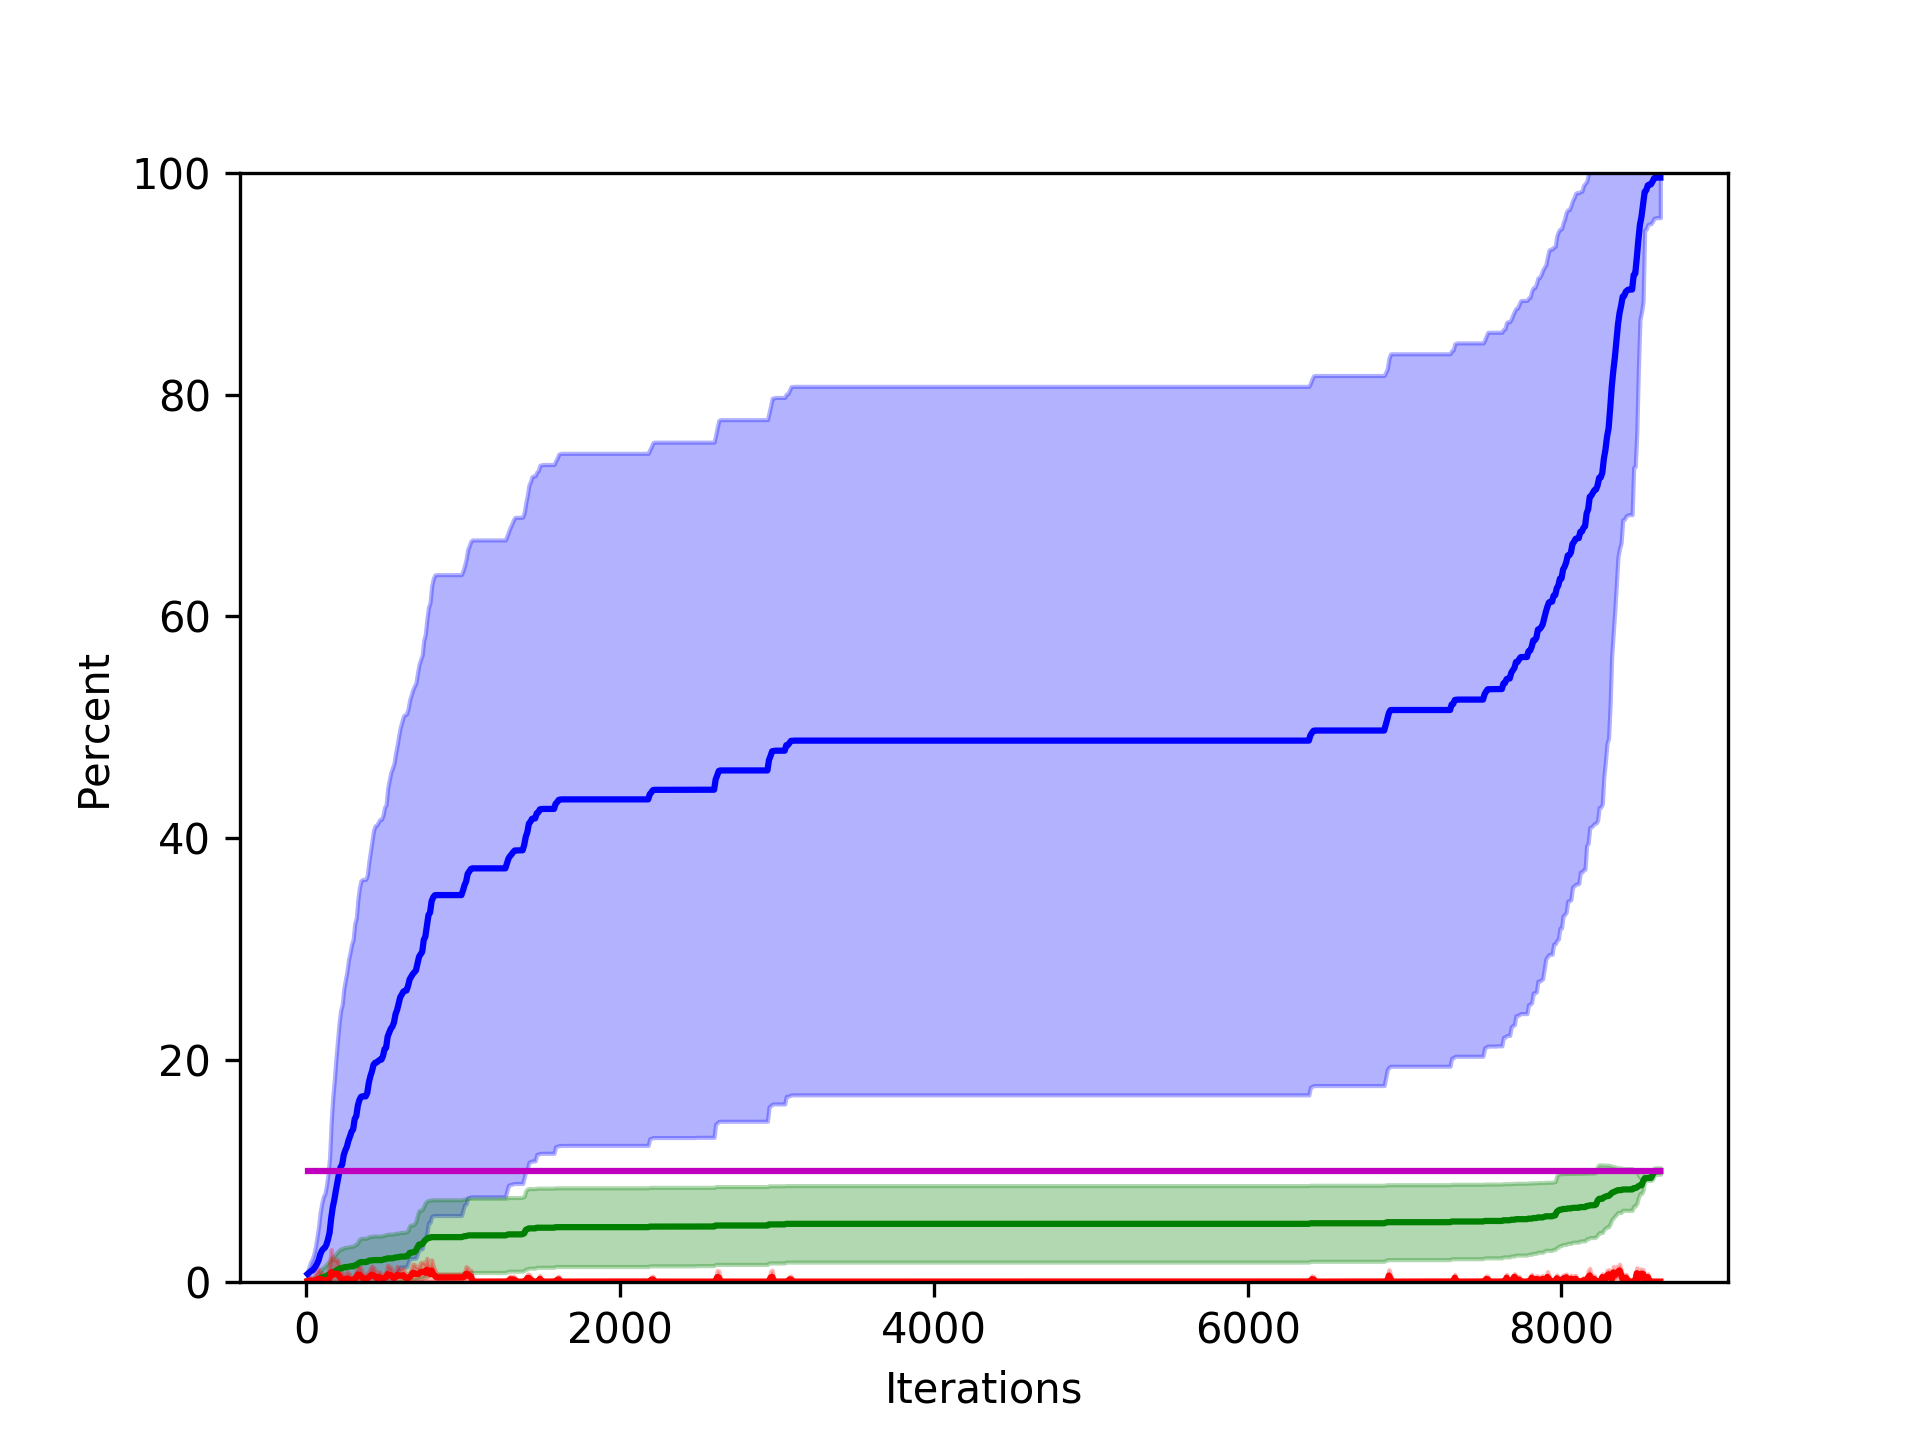
\includegraphics[width=\linewidth]{images/plots/Network_rA_10.0/new_plots/10_10.png}
\caption{$\rho$ = 10m.} \label{fig:tarjan0}
\end{subfigure}

\begin{subfigure}{0.6\textwidth}
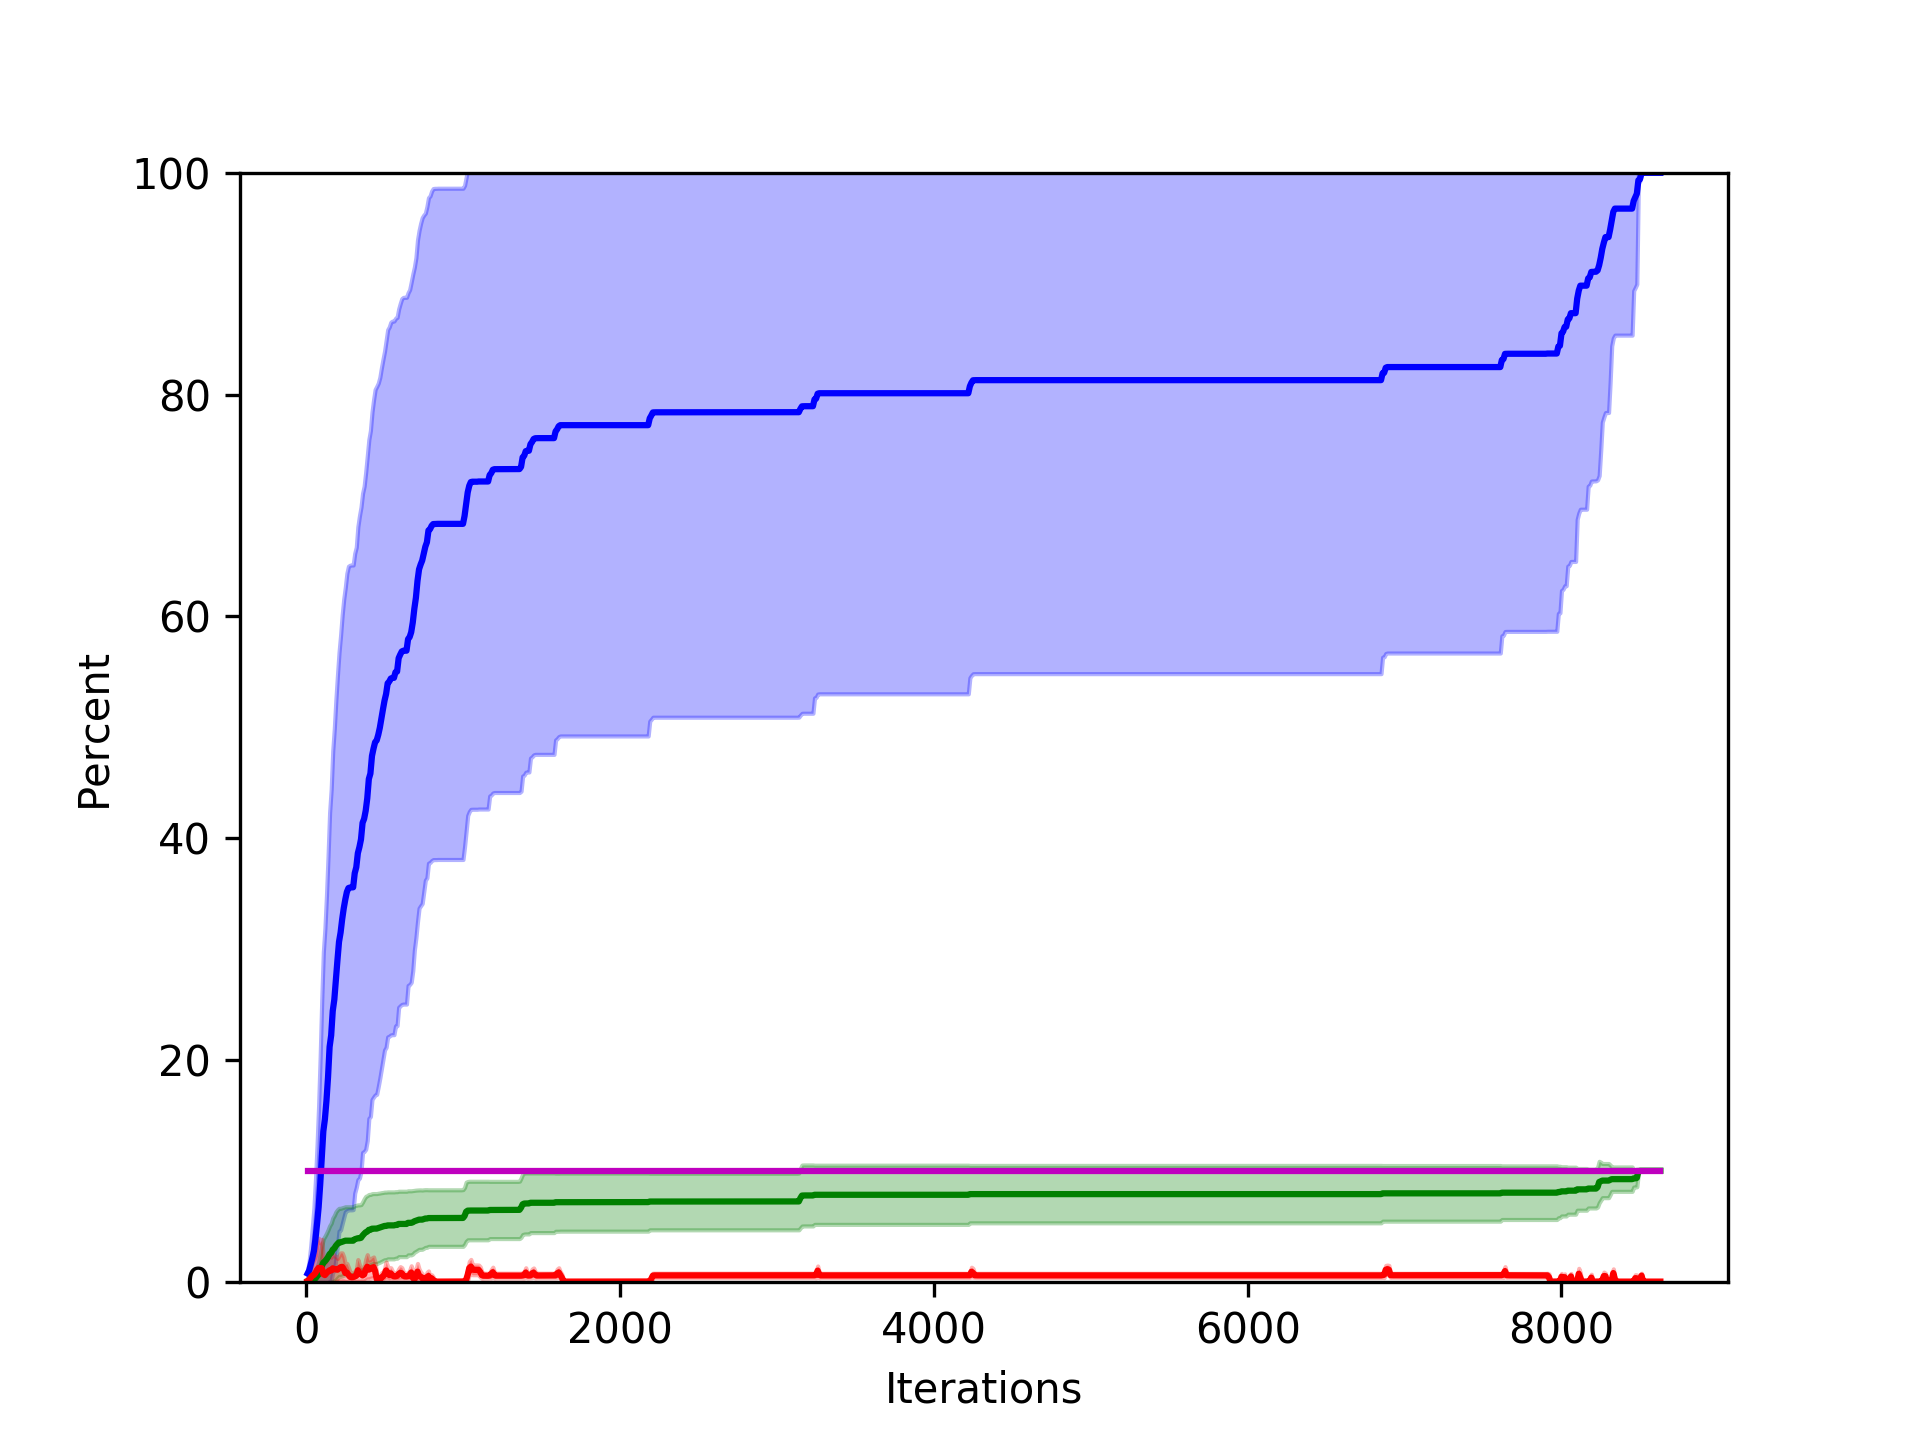
\includegraphics[width=\linewidth]{images/plots/Network_rA_10.0/new_plots/30_10.png}
\caption{$\rho$ = 30m.} \label{fig:tarjan0}
\end{subfigure}

\begin{subfigure}{0.6\textwidth}
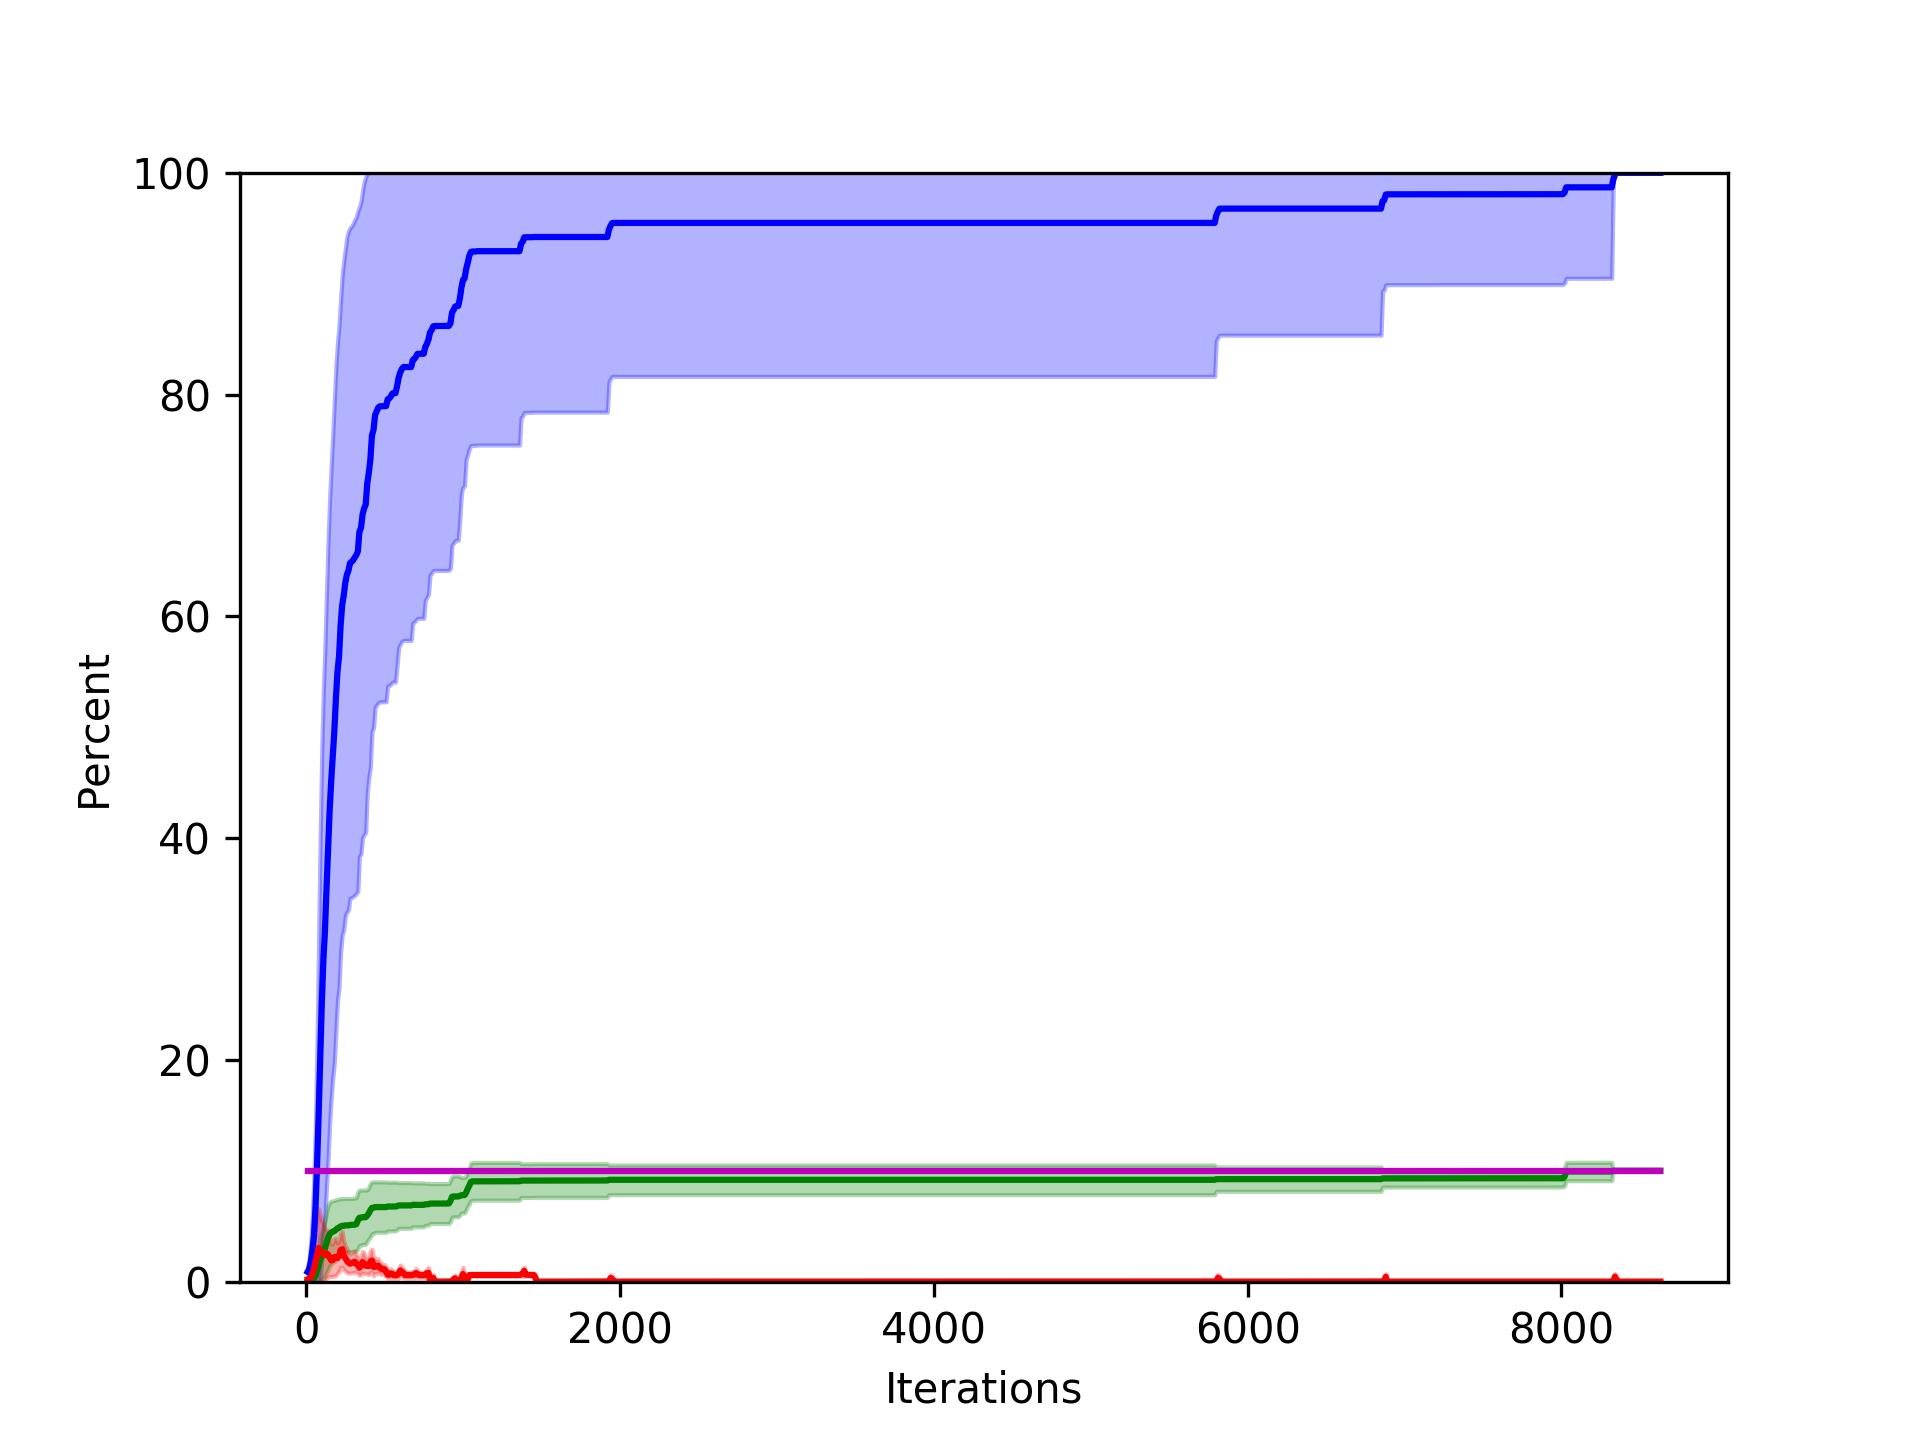
\includegraphics[width=\linewidth]{images/plots/Network_rA_10.0/new_plots/50_10.png}
\caption{$\rho$ = 50m.} \label{fig:tarjan0}
\end{subfigure}

\caption{Simulation with 10\% malicious nodes and varying values of $\rho$.}
\label{fig:random103050}
\end{figure}



\begin{figure}
\centering

\begin{subfigure}{0.45\textwidth}
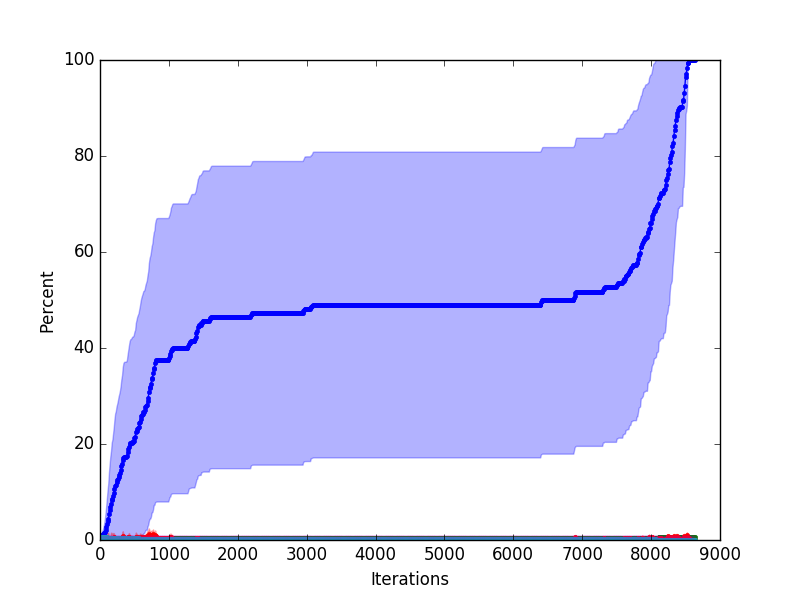
\includegraphics[width=\linewidth]{images/plots/Network_rA/10_1.png}
\caption{1\% malicious.}
\end{subfigure}
\hspace*{0.1cm} % separation between the subfigures
\begin{subfigure}{0.45\textwidth}
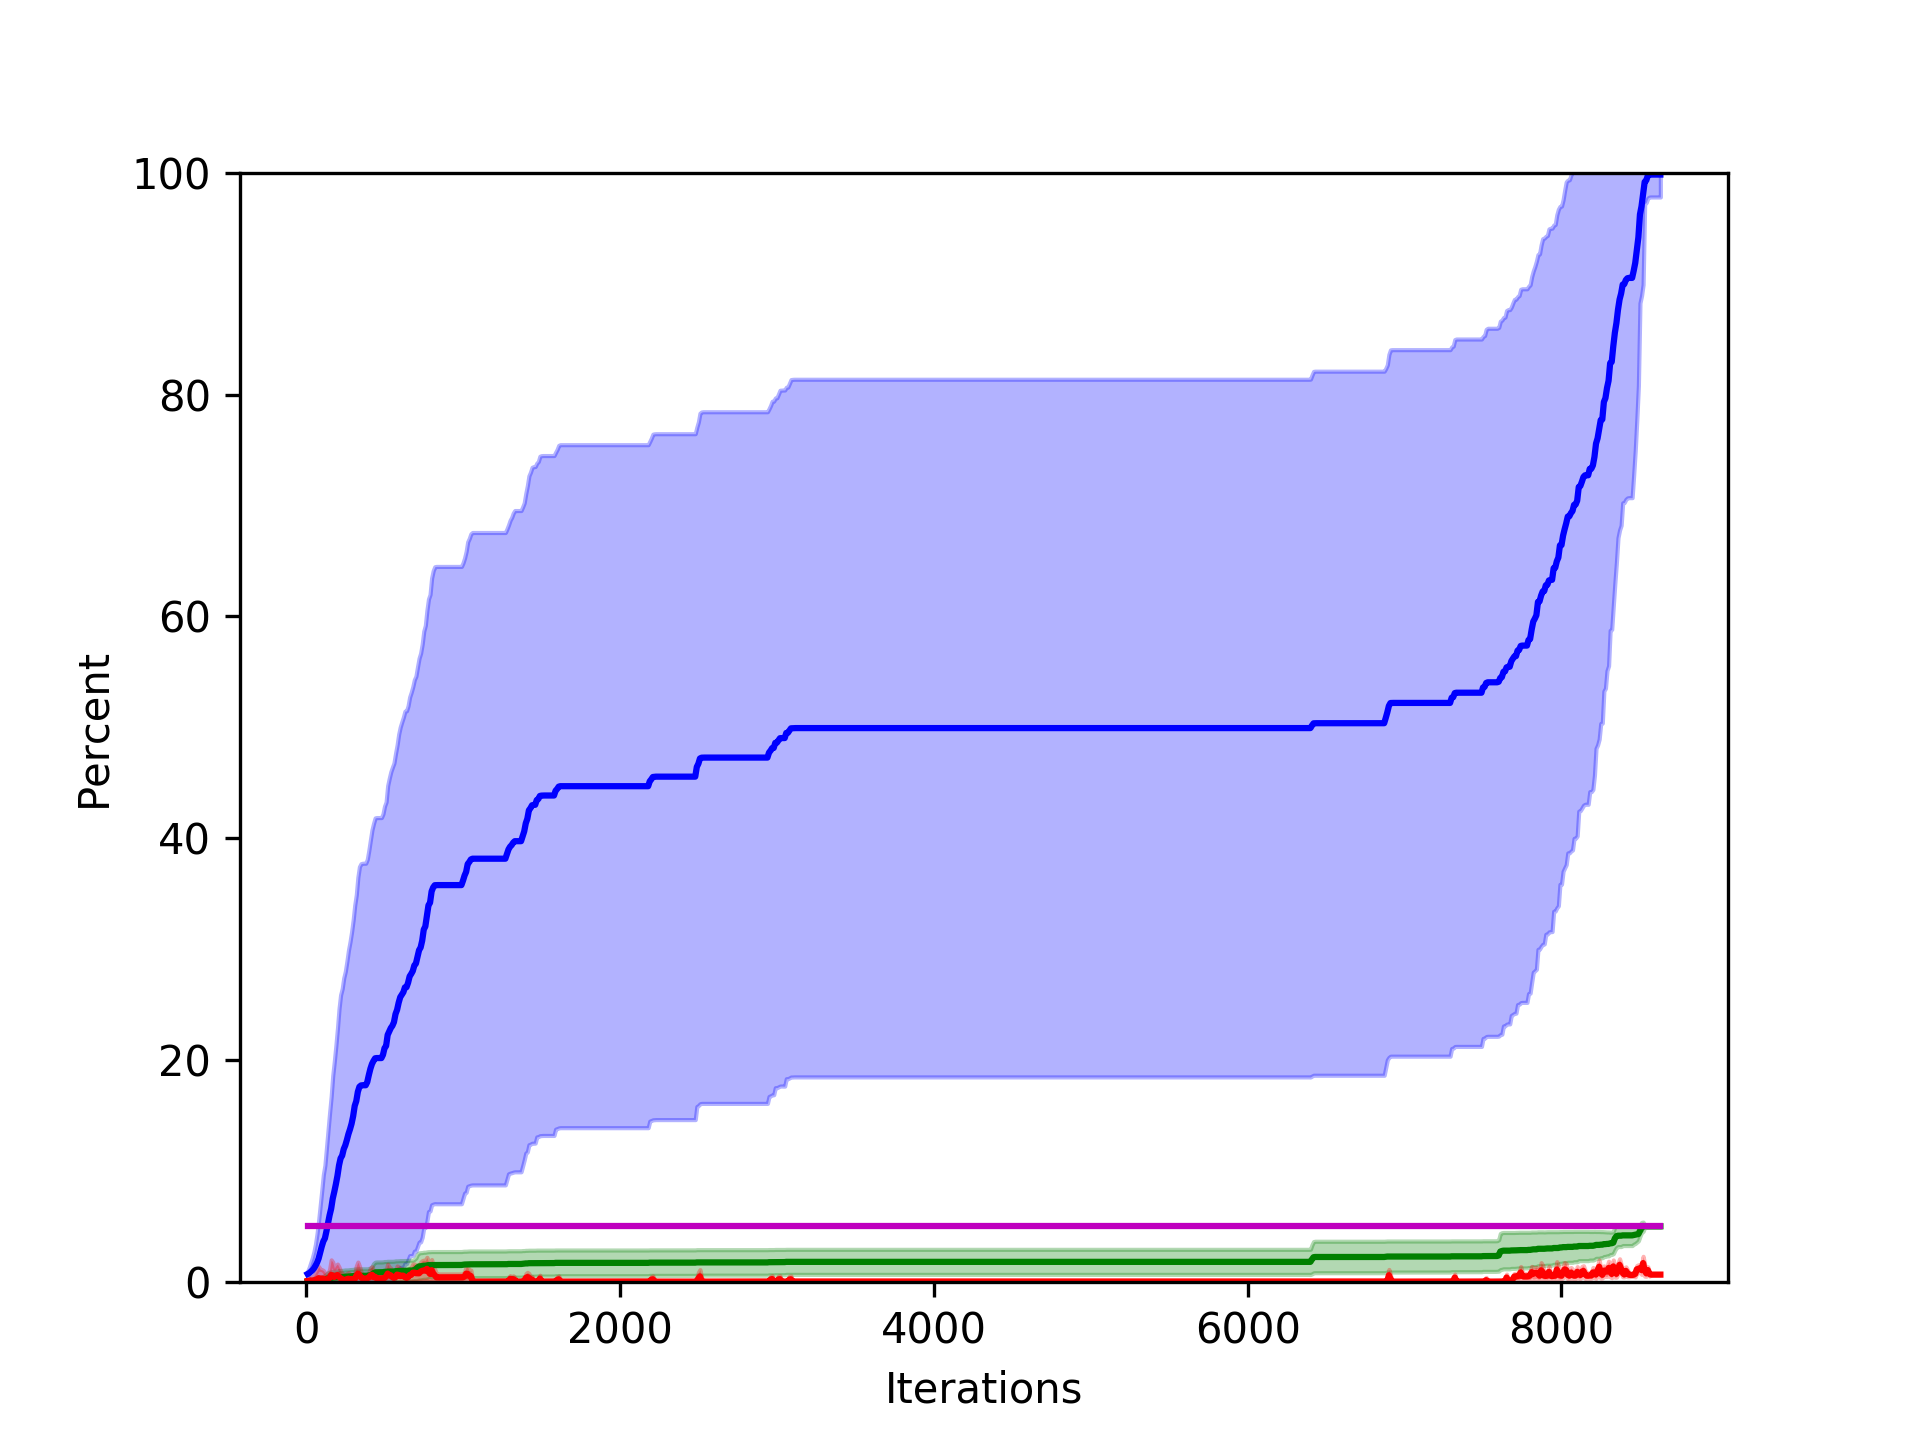
\includegraphics[width=\linewidth]{images/plots/Network_rA/10_5.png}
\caption{5\% malicious.}
\end{subfigure}

\vspace{1cm}

\begin{subfigure}{0.45\textwidth}
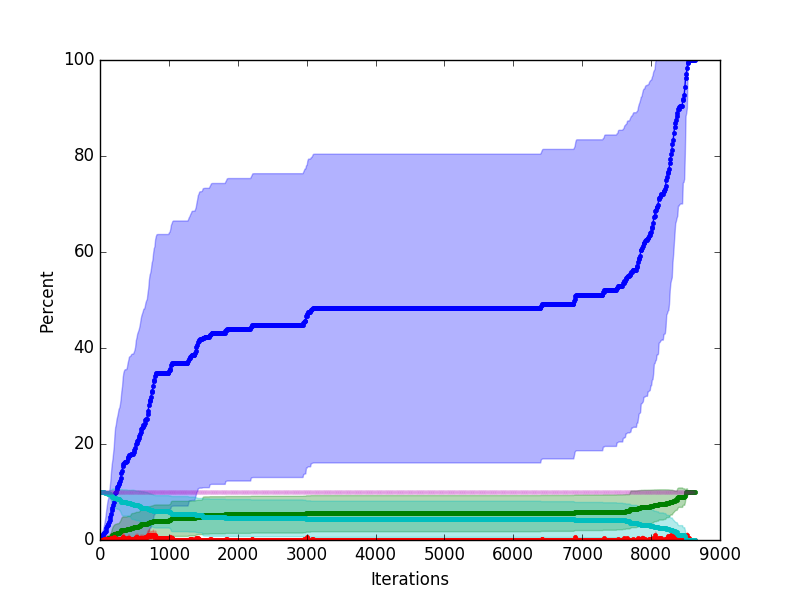
\includegraphics[width=\linewidth]{images/plots/Network_rA/10_10.png}
\caption{10\% malicious.}
\end{subfigure}
\hspace*{0.1cm} % separation between the subfigures
\begin{subfigure}{0.45\textwidth}
\includegraphics[width=\linewidth]{images/plots/Network_rA/10_30.png}
\caption{30\% malicious.}
\end{subfigure}

\vspace{1cm}

\begin{subfigure}{0.45\textwidth}
\includegraphics[width=\linewidth]{images/plots/Network_rA/10_40.png}
\caption{40\% malicious.}
\end{subfigure}
\hspace*{0.1cm} % separation between the subfigures
\begin{subfigure}{0.45\textwidth}
\includegraphics[width=\linewidth]{images/plots/Network_rA/10_50.png}
\caption{50\% malicious.}
\end{subfigure}

\caption{Simulation with $\rho$ = 10m and varying percentages of malicious nodes.}
\label{fig:randommalicious}
\end{figure}


\begin{figure}
\centering

\begin{subfigure}{0.5\textwidth}
\includegraphics[width=\linewidth]{images/plots/thresholds/03_30_10}
\caption{$h = 0.3$.} \label{fig:tarjan0}
\end{subfigure}

\begin{subfigure}{0.5\textwidth}
\includegraphics[width=\linewidth]{images/plots/thresholds/05_30_10}
\caption{$h = 0.5$.} \label{fig:tarjan0}
\end{subfigure}

\begin{subfigure}{0.5\textwidth}
\includegraphics[width=\linewidth]{images/plots/thresholds/07_30_10}
\caption{$h = 0.7$.} \label{fig:tarjan0}
\end{subfigure}

\caption{Simulation with 10\% malicious nodes, $\rho = 30$m and varying values of $h$.}
\label{fig:randomthresholds}
\end{figure}


\begin{figure}
\centering
\includegraphics[width=\textwidth]{images/plots/Network_rA7/10_10}
\caption{7 days scenario: 10m range and 10\% malicious nodes.} \label{fig:random7}
\end{figure}

%\begin{figure}
%\centering
%
%\begin{subfigure}{0.4\textwidth}
%\includegraphics[width=\linewidth]{images/plots/Network_rA/10_1.png}
%\caption{1\% malicious.} \label{fig:tarjan0}
%\end{subfigure}
%
%\hspace*{1cm}
%
%\begin{subfigure}{0.4\textwidth}
%\includegraphics[width=\linewidth]{images/plots/Network_rA/10_5.png}
%\caption{5\% malicious.} \label{fig:tarjan0}
%\end{subfigure}
%
%\vspace{1cm}
%
%\begin{subfigure}{0.5\textwidth}
%\includegraphics[width=\linewidth]{images/plots/Network_rA/10_10}
%\caption{10\% malicious.} \label{fig:tarjan0}
%\end{subfigure}
%
%\hspace*{\fill}
%
%\begin{subfigure}{0.5\textwidth}
%\includegraphics[width=\linewidth]{images/plots/Network_rA/10_10}
%\caption{$\rho$ = 50m.} \label{fig:tarjan0}
%\end{subfigure}
%
%\vspace{1cm}
%
%\begin{subfigure}{0.5\textwidth}
%\includegraphics[width=\linewidth]{images/plots/Network_rA/10_10}
%\caption{$\rho$ = 50m.} \label{fig:tarjan0}
%\end{subfigure}
%
%\hspace*{\fill}
%
%\begin{subfigure}{0.5\textwidth}
%\includegraphics[width=\linewidth]{images/plots/Network_rA/10_10}
%\caption{$\rho$ = 50m.} \label{fig:tarjan0}
%\end{subfigure}
%
%\caption{Simulation with $\rho$ = 10m varying malicious.}
%\label{fig:random0}
%\end{figure}

%\begin{figure*}[!t]
%\centering
%\subfloat[]{\includegraphics[width=0.329\linewidth]{images/plots/Network_rA/10_1}%
%\label{subfig:random1}}
%\hfil
%\subfloat[]{\includegraphics[width=0.329\linewidth]{images/plots/Network_rA/10_5}%
%\label{subfig:random2}}
%\hfil
%\subfloat[]{\includegraphics[width=0.329\linewidth]{images/plots/Network_rA/10_10}%
%\label{subfig:random3}}
%
%\subfloat[]{\includegraphics[width=0.329\linewidth]{images/plots/Network_rA/10_30}%
%\label{subfig:random4}}
%\hfil
%\subfloat[]{\includegraphics[width=0.329\linewidth]{images/plots/Network_rA/10_40}%
%\label{subfig:random5}}
%\hfil
%\subfloat[]{\includegraphics[width=0.329\linewidth]{images/plots/Network_rA/10_50}%
%\label{subfig:random6}}
%
%\caption{Simulation with $\rho$ = 10m and (a) 1\%, (b) 5\%, (c) 10\%, (d) 30\%, (e) 40\% or (f) 50\% malicious.}
%\label{fig:random0}
%\end{figure*}
	% validação
\chapter{Conclusion}
\label{chap:conclusion}

In the coming years, vehicular networks or VANETs will be an important part of safety and security in transportation, optimizing traffic and reducing the number of accidents.
However, they are an appealing target for entities with malicious intents, creating the need of robust solutions to maintain the integrity of such networks.

The concept of trust as applied in VANETs is a powerful tool for those seeking to reduce the spread of false information among members of a network as much as possible.
In this paper, a new trust model for vehicular networks called TruMan was introduced, which combines the efficiency of previously proposed algorithms in order to generate fast and accurate results.
The solution works in a decentralized fashion and is built for the dynamic environment of vehicular networks, although it could also be adapted to other types of networks.

As nodes travel across the network and collect more data from neighbors, they are able to form an abstraction of the network which can be used to detect malicious nodes.
By placing nodes into strongly connected components, a network containing a large amount of nodes can be simplified into a much smaller one.
Using a simple graph coloring algorithm, most malicious nodes stand out by having different colors than the majority of nodes.
This allows for a low complexity approach to malicious node identification in a dynamic network.

TruMan was evaluated using mobility data gathered from the ONE simulator using the Working Day Movement Model, which approximates node mobility to that of real-world vehicles.
Several simulations were performed, changing certain parameters to understand how the model performs in different scenarios.
The experiments show that vehicles within a network can form a sufficient abstraction of the network in around one day, and with that information they are able to detect nearly every malicious node in the network, with a very small amount of false positives.
As the network changes in shape, nodes acquire more information and are able to make even more accurate classifications of malicious nodes around them.
With the implementation of information aging, TruMan is also able to detect nodes that start benign and become malicious during the simulation.

In comparison with the related work, TruMan was able to satisfy most of the desired properties for vehicular network trust models, while not inhibiting the properties that were not desired.
Most importantly, TruMan put emphasis on efficiency and is the first model that clearly displays the complexity of its algorithm.
Furthermore, TruMan begins taking advantage of social network features found in vehicular networks, although more can be done with this idea.

The work done on TruMan was published as a conference paper on the 2018 IEEE Symposium on Computers and Communications \citep{greca2018truman}.

\pagebreak
Several paths could be considered for future work on TruMan, such as:
\begin{itemize}
\item TruMan could be tested in more varied scenarios, using different maps and various different amounts of nodes in the simulations. It would be even better to use real-world mobility data.
\item TruMan takes advantage of social features found in vehicular networks, but even more could be done with this. For example, vehicles that belong to the same family could have strong ties and share a lot of data with each other. Certain vehicles, such as police cars and ambulances, could have privileged roles within the model.
\item The model could be adapted to include public transportation vehicles (trains, buses) with predictable routes, as well as vehicle-to-infrastructure communication.
\item Well-known vehicular network attacks, such as the ones in \citep{isaac2010security}, could be used against TruMan, attempting to break it. Such experiments would fully validate TruMan's robustness.
\item TruMan should be tested in real-world networks. Although it was designed for vehicular networks, other types of networks with mobility, such as mobile ad-hoc networks, could be used for experiments.
\item Finally, it is possible that TruMan might be a valuable tool for more than just vehicular network. A decentralized and dynamic trust management scheme could be useful for social networks, mobile ad-hoc networks, Internet-based peer-to-peer networks, and others. These scenarios should be tested.
\end{itemize}



%Rede complexas: métricas (dinâmica)? Grafo de Componentes para reduzir a complexidade da rede
%
%Limitações do One? Dtn
%Preservação da rede (slide) mesmo sem alcance da comunicação?
%
%Trust: trusted vehicles (minhas 2010)
%
%Fog computing: cluster em bus stops ou rsup
%
%Contribuição: correção & eficiência, redes sociais wdmm, rotina,
%
%Janela de tempo para descoberta e atualização dinâmica da topologia- execução dos 3 passos seguintes (limitação do tempo - iteração?) alguma frequência ? F(v, d)
%M ? 
%
%
%Diagnóstico (ok - fora do escopo) - sem análise do teste do nó.
%
%Noticias boas mais rápido que más: retirada da aresta?
%Modelo de ataques?

		% conclusão

%=====================================================

% Estilos de bibliografia recomendados (só descomentar um estilo!)
%\bibliographystyle{apalike}	% [Maziero et al., 2006]
%\bibliographystyle{plain}		% [1], [1, 2]
%\bibliographystyle{alpha}		% [Maz06], ...
\bibliographystyle{plainnat}		% vide Google "LaTeX Natbib"

% base de bibliografia (BibTeX)
\bibliography{refs, dissertation}
%\bibliography{file1, file2, file3} % se tiver mais de um arquivo BibTeX

%=====================================================

% apêndices
%\appendix
%\include{a1-exemplo/exemplo}

\end{document}

%=====================================================